% Latex Template
% Politechnika Gdańska - Szablon Pracy Dyplomowej (Inżynierskiej/Magisterskiej)
% first version by Kamil Trzebiatowski
% this version: 2019.09.17
% Compiler: XeLaTex
% insert your chapters in: Chapters/ChaptersMain.tex
% insert your appendices in: Appendices/AppendicesMain.tex

% Bibliography manager: BibLaTex
% insert bibliography items in: bibliografia.bib

%  !-- Do not edit this file unless you know what you do. --! %

\documentclass[10pt, twoside, polish]{report}
\usepackage{listings}
\usepackage{xcolor}

\definecolor{codegreen}{rgb}{0,0.6,0}
\definecolor{codegray}{rgb}{0.5,0.5,0.5}
\definecolor{codepurple}{rgb}{0.58,0,0.82}
\definecolor{backcolour}{rgb}{0.95,0.95,0.92}


\lstset{emph={
    delete
    }, emphstyle={\color{magenta}}
}

\lstdefinestyle{mystyle}{
    backgroundcolor=\color{backcolour},   
    commentstyle=\color{codegreen},
    keywordstyle=\color{magenta},
    numberstyle=\tiny\color{codegray},
    stringstyle=\color{codepurple},
    basicstyle=\ttfamily\footnotesize,
    breakatwhitespace=false,         
    breaklines=true,                 
    captionpos=b,                    
    keepspaces=true,                 
    numbers=left,                    
    numbersep=5pt,                  
    showspaces=true,                
    showstringspaces=false,
    showtabs=true,                  
    tabsize=2
}

\lstset{style=mystyle}

\usepackage[utf8]{inputenc} % Required for inputting international characters
%\usepackage{polski}
%\usepackage[polish]{babel}

\usepackage[T1]{fontenc} % Output font encoding for international characters

\usepackage{blindtext}
\usepackage{geometry}
\usepackage{indentfirst}

\usepackage{amsmath} %paczka do rownan
\renewcommand{\theequation}{\thechapter.\arabic{equation}} %rownania postaci 2.1, 3.2

\usepackage{textgreek} %inline greek characters

% ladowanie grafiki
\usepackage{graphicx}
\graphicspath{ {Images/} } %sciezka do obrazkow

\usepackage{float}
%
\usepackage{wrapfig}

\usepackage{caption}
\usepackage{subcaption}


\newcommand\tab[1][1cm]{\hspace*{#1}}%komenda - tabulator, uzycie: tab[x], gdzie x jest dlugoscia akapitu
\newcommand*{\noaddvspace}{\renewcommand*{\addvspace}[1]{}}

% formatowanie wyliczen (listy kropkowanej)
\usepackage{enumitem}
\setlist[itemize]{noitemsep, topsep=0pt}
%

% FORMATOWANIE NAGLOWKOW %
\usepackage[explicit]{titlesec}
\usepackage{lipsum}
%%%%%
%FORMATOWANIE PRZYPISOW
\renewcommand{\footnotesize}{\small}
\usepackage{chngcntr}
\counterwithout{footnote}{chapter}
%%%%

\usepackage[toc,page]{appendix}

% WCZYTANIE PLIKU BIBLIOGRAFII
\usepackage[backend=biber, style=numeric-comp, sorting=none, maxnames=4, minnames=2, maxbibnames=99]{biblatex}

\addbibresource{bibliografia.bib}
\usepackage{csquotes}

% FORMATOWANIE WPISÓW BIBLIOGRAFII %
\renewcommand*{\finalnamedelim}{\multinamedelim} %usuniecie finalnego 'i'

\renewbibmacro*{volume+number+eid}{%
\iffieldundef{volume}{}{,\space vol.
  \printfield{volume}%
  \iffieldundef{number}{}{\setunit*{\addspace}%
,\space nr
  \printfield{number}%,
,
  \setunit{\addcomma\space}%
  \printfield{eid}}}
}

\DefineBibliographyStrings{polish}{andothers = {\textit{et\addabbrvspace al\adddot}}}

%\DeclareFieldFormat[article]{volume}{,vol. #1 }
%\DeclareFieldFormat[article]{number}{ nr #1}

\DeclareFieldFormat[article]{citetitle}{#1}
\DeclareFieldFormat[article]{title}{#1}

\renewbibmacro{title}{%
  \ifentrytype{article}{\textit{\printfield{title}}}{\printfield{title}}
}

\renewbibmacro*{issue+date}{%
  \setunit{\addcomma\space}% NEW
%  \printtext[parens]{% DELETED
    \iffieldundef{issue}
      {\usebibmacro{date}}
      {\printfield{issue}%
       \setunit*{\addspace}%
%       \usebibmacro{date}}}% DELETED
       \usebibmacro{date}}% NEW
  \newunit}

\DeclareFieldFormat{journaltitle}{#1} % normal journal title

\renewbibmacro{in:}{%
  \ifentrytype{article}
    {}
    {\printtext{\bibstring{in}\intitlepunct}}}

\usepackage{hyperref}
\usepackage{bookmark}
\def\UrlBreaks{\do\/\do-}
% Format Bibliography @online articles
\usepackage{color}
%\usepackage{url}
\urlstyle{same}
\DefineBibliographyStrings{polish}{urlseen = {data dostępu:}}
\DeclareFieldFormat{url}{\color{blue}\url{#1}}
\DeclareFieldFormat{doi}{\newline\color{blue}\href{https://doi.org/#1}{doi:#1}}
%\DeclareFieldFormat{url}{\url{#1}}
% ------------------------------------------------ %

% ------------------------------------------------ %
%%   formatowanie naglowkow, kropki po numeracji  %%
%88888888888888888888%
\usepackage{nameref}
\makeatletter
\newcommand*{\currentname}{\@currentlabelname}
%88888888888888888888%


\titleformat{\chapter}
{\large\bfseries}
{\thechapter.}{0.5em}{\MakeUppercase{#1}}

\titleformat{\section}
{\normalfont\bfseries\itshape}
{\thesection.}{0.5em}{#1}

\titleformat{\subsection}
{\normalfont\itshape}
{\thesubsection.}{0.5em}{#1}
%------------------------------%

%% POLSKIE NAZWY - ZMIANA NA WYMAGANE %%
\addto\captionspolish{\renewcommand{\listtablename}{\textbf{Wykaz tabel}}}
\addto\captionspolish{\renewcommand{\listfigurename}{\textbf{Wykaz rysunków}}}

\addto\captionspolish{\renewcommand{\bibname}{\textbf{Wykaz literatury}}}
\renewcommand\bibname{Wykaz literatury}
\addto\captionspolish{\renewcommand{\refname}{\textbf{Wykaz literatury}}}
\renewcommand\refname{Wykaz literatury}

\addto\captionspolish{\renewcommand{\appendixname}{Dodatek}}
%% --------------------------------------------------- %%

% FORMATOWANIE PODPISOW POD OBRAZKAMI %
\usepackage{caption,setspace}
\usepackage{subcaption}
\addto\captionspolish{\renewcommand{\figurename}{Rys.}}
\captionsetup{labelsep=period}

\captionsetup{font={small, stretch=1.0}}     		%  FONT 9 pt Interlinia 1 pt
\captionsetup{belowskip=12pt,aboveskip=6pt}%Górny odstęp akapitu powinien być ustawiony na wartość 6 pkt, a dolny 12 pkt
\captionsetup{justification=centering}		% wysrodkowanie
%\renewcommand{\thefigure}{\thechapter\arabic{figure}} % set caption label style to 1.1.
\setlength{\belowcaptionskip}{0pt}
\setlength{\floatsep}{0pt}
\setlength{\intextsep}{10pt}
\setlength{\textfloatsep}{10pt}

%--------------%%%%%%%%%%--------------%

% FORMATOWANIE PODPISOW NAD TABELAMI %
\addto\captionspolish{\renewcommand{\tablename}{Tabela}}

%\captionsetup[table]{belowskip=0pt,aboveskip=6pt}%Górny odstęp akapitu powinien być ustawiony na wartość 6 pkt, a dolny 0 pkt
%\captionsetup[table]{justification=justified}		

 \captionsetup[table]{
  labelsep = newline,
font={small, stretch=1.1}, %  FONT 9 pt Interlinia ~1.1 pt
  justification=justified,% wyrownanie  do lewej
  singlelinecheck=false,%%%%%%% a single line is centered by default
  labelsep=period,%%%%%%
  belowskip=0pt, % skip pod/nad tabela
  aboveskip=6pt,% skip pod/nad tabela
  skip = 1.5mm, %skip pod nazwa tabeli
}

%\renewcommand{\thetable}{\thechapter\arabic{table}.} % set caption label style to 1.1.

\usepackage{tabularx}
\renewcommand{\arraystretch}{1.4} %wysokosc wiersza TABELI (teraz ok. 0,5 cm)
%--------------%%%%%%%%%%--------------%

% HEADER, FOOTER FORMATTING %
\usepackage{fancyhdr}
\fancypagestyle{plain}{%
\fancyhf{} % clear all header and footer fields
\fancyfoot[C]{\small\thepage} % WYSRODKOWANY, 9 PT
\renewcommand{\headrulewidth}{0pt}
\renewcommand{\footrulewidth}{0pt}}
\pagestyle{plain}
% ---------------------------------------%

%-------- FORMATOWANIE SPISU TRESCI --------%
\usepackage[dotinlabels]{titletoc}

%\usepackage[nottoc]{tocbibind}
%\usepackage{afterpage}

\titlecontents{chapter}[0cm]{}{\normalsize\bfseries\contentslabel{-1pt}\hspace*{0.6cm}}{}{\titlerule*[3pt]{.}\hspace*{5pt}\contentspage}

\titlecontents{section}[0.6cm]{}{\normalsize\contentslabel{-1pt}\hspace*{0.9cm}}{}{\titlerule*[3pt]{.}\hspace*{5pt}\contentspage}

\titlecontents{subsection}
  [1.5cm]{}{\normalsize\contentslabel{-1pt}\hspace*{1.4cm}}{}{\titlerule*[3pt]{.}\hspace*{5pt}\contentspage}

\usepackage{listings}
\usepackage{courier}
\lstset{basicstyle=\footnotesize\ttfamily,breaklines=true}
\lstset{
  basicstyle = \footnotesize\ttfamily,
  basewidth  = {.5em,0.5em},
  breaklines = true,
  % columns  = flexible,
  % columns  = fullflexible,
}
% --------------------------------------------------------%

%- FORMATOWANIE LIST OF TABLES, LIST OF FIGURES -%
\titlecontents{figure}[0cm]{}{\normalsize\contentslabel{-1pt}\hspace*{1cm}}{}{\titlerule*[3pt]{.}\hspace*{5pt}\contentspage}
\titlecontents{table}[0cm]{}{\normalsize\contentslabel{-1pt}\hspace*{1cm}}{}{\titlerule*[3pt]{.}\hspace*{5pt}\contentspage}
% --------------------------------------------------------%

% POPRAWKA NA MARGINESY (akapity) TYTUŁÓW %
\titlespacing*{\chapter}{0pt}{-20pt}{6pt}
\titlespacing*{name=\chapter,numberless}{0pt}{-20pt}{6pt}

\titlespacing*{\section}{0pt}{12pt}{6pt}
\titlespacing*{\subsection}{0pt}{12pt}{6pt}
%  -------------------------------------------------------- %

%\usepackage{showframe}
%% FONTY
\usepackage{unicode-math}
\usepackage{fontspec}
\setmainfont{Arial}
\usepackage{pdfpages}
% Alternative Math fonts - change to yours or uncomment something %
%\usepackage[varg]{txfonts}
%\usepackage{newtxtext}
%\usepackage{newtxmath}
%\usepackage{newtxmath}
%\setmathfont{[mathfont.ttf]}
%\setmathfont{Computer Modern}
% --------------------------------------------------------------- %
\usepackage{multirow}
%\usepackage{multicolumn}

\addtocontents{toc}{\protect\noaddvspace}
\renewcommand{\baselinestretch}{1.45} %1,5 wiersza interlinii (wzór=ms word)
\setlength{\parindent}{4em}
\setlength{\parskip}{1em}

\title{
	{Praca/Projekt dyplomowa/y magisterska/inżynierski - szablon LATEX
    }\\
	{\large Politechnika Gdańska}\\
	{\includegraphics{pg_logo.jpg}}
}
\author{Kamil Trzebiatowski - 2019}
\date{\textbf{[PLACEHOLDER - Tę stronę należy zastąpić wydrukiem z Moja PG]}}

\geometry{
	paper=a4paper, % A4
	inner=3.5cm, % Inner margin
	outer=2.5cm, % Outer margin
	bindingoffset=0cm, % Binding offset
	top=2.5cm, % Top margin
	bottom=2.5cm, % Bottom margin
	footskip=1cm, % polozenie stopki
	%showframe % Uncomment to show how the type block is set on the page
}

%%%%%% WLASCIWY DOKUMENT - START %%%%%%
%%%%%% -------------------------------------- %%%%%%
\begin{document}
 
% STRONA TYTULOWA PRACY DYPLOMOWEJ - s 1, numer niewidoczny
% \begin{titlepage}
% \pagestyle{plain}
% \pagenumbering{arabic}
% \setcounter{page}{1}
% \maketitle
% \end{titlepage}

\includepdf[pages={1}]{titlepage.pdf}
\setlength{\parskip}{0pt}
% OSWIADCZENIE AUTORA PRACY - s 2, numer niewidoczny
% \chapter*{Deklaracja zgodności}
% \normalsize
% Deklaruję zgodność produktu z dyrektywą 2006/112/UE oraz 2014/35/UE i normami PN-EN 1176-1:2009, PN-EN 1939:2007.\par\textbf{[PLACEHOLDER - Tę stronę należy zastąpić wydrukiem z Moja PG]}

\includepdf[pages={1}]{statement.pdf}
% STRESZCZENIE  - s 3, numer widoczny
\chapter*{Streszczenie}
Sieci informacjo-centryczne (ang. Information-centric Networking (ICN))––które kandydują do miana sieci przyszłości––zmagają się z nowym wektorem ataków. Jednym z ataków jest atak zatruwania treści (ang. Content Posioning Attack (CPA)), a zwłaszcza jego silniejsza forma––atak zatruwania treści przez fałszywe dane (ang. Fake Data CPA). Sieci te, są wyjątkowo podatne na ten typ ataków, ponieważ nie pozwalają na usuwanie treści––w momencie, gdy treść trafia do sieci, nie jest możliwe jej usunięcie inaczej niż poprzez wygaśnięcie.
Aktualnie znane metody uwierzytelniania jak login/hasło, klucze prywatne, biometria, potwierdzenie SMS/email operują w jednym tym samym wymiarze uwierzytelniania. W tej pracy proponujemy nowy wymiar uwierzytelniania, który bazuje na dostępnie do czasu. Kiedy napastnik-wydawca operuje w czasowo ograniczonym środowisku, jego dostęp do skradzionych uwierzytelnień jest czasowo ograniczony, podczas gdy prawdziwy wydawca nie jest ograniczony czasowo w żaden sposób. Ta różnica jest wykorzystana w celu stworzenia nowego systemu uwierzytelniania.
Dwie implementacje systemu są zaproponowane, pierwsza bazuje na algorytmie infekcji na grafach, a druga na łańcuchu bloków (ang. Blockchain). Dzięki zbudowanym symulatorom jesteśmy w stanie zaobserwować problem Sojuszu Obronnego (ang. Deffensive Alliance) w algorytmie infekcji na grafach.
Obie metody zostają ocenione pod kątem złożoności komunikacyjnej, determinizmowi algorytmów, możliwości dopasowania się do zmian, oraz odporności na błędy (również silniejszej formy bizantyjskich generałów).

% ABSTRACT - s 4, numer widoczny,
\chapter*{Abstract}
Information-centric networks––that are candidates for the title of the network of the future––struggle with a new vector of attacks. One of them is content poisoning, especially the stronger form––Fake Data CPA. ICN networks are especially prone to those types of attacks due to a lack of removal functionality. Currently, known authentication methods like login/password, private key, biometry, SMS/email confirmation operate on the same dimension of authentication. We propose a new authentication dimension, which is time availability. When an adversary publisher is operating in a time-constrained environment, his access to target credentials is limited, whereas honest publisher is not timely constrained in any way. We leverage such distinction to propose a new authentication mechanism.
Two implementations are proposed, the first one based on infection processes in graphs, and the second one based on blockchain technology. We provide simulators that give us interesting observations, such as the Defensive Alliance problem in graph infection algorithm. We evaluate both approaches in terms of communication complexity, scalability, determinism, resilience, and fault-tolerance (including its stronger form––Byzantine-fault).

% SPIS TREŚCI - s 5, numer widoczny
\setcounter{tocdepth}{2}
\clearpage
\phantomsection
\pdfbookmark{\contentsname}{Table of Contents}
\tableofcontents

% Wykaz ważniejszych oznaczeń i skrótów
\chapter*{List of important symbols and abbreviations}
\addcontentsline{toc}{chapter}{\bfseries List of important symbols and abbreviations}
\begin{tabbing}

  \textbf{NDO}\tab[3cm] \=-- Named Data Object, an object primitive used in NDN networks.\\
  \textbf{ICN} \>-- Information-centric network.\\
  \textbf{NDN} \>-- Named Data Networking.\\
  \textbf{CPA} \>-- Content Poisoning Attack.\\
  \textbf{Fake Data CPA} \>-- A stronger form of Content Poisoning Attack where the adversary has access \\
  \>   to credentials and can forge valid signature on poisoned data.\\
  \textbf{WoT} \>-- Web of trust graph generator.\\
  \textbf{PB} \>-- Probabilistic duplication graph generator.\\
  \textbf{RNG} \>-- Random graph generator.\\
  \textbf{Proof-of-Time} \>-- Proof of access to credentials over some period.\\
  \textbf{Credibility Score} \>-- Number of collected proof-of-time claims over total required number of proof-of-times.\\
  \textbf{GI} \>-- Graph Infection algorithm \cite{konorski2019mitigating}.\\
  \textbf{FBA} \>-- Federated Byzantine Agreement consensus protocol \cite{mazieres2015stellar}.\\
  \textbf{SCP} \>-- Stellar Consensus Protocol, the construction of FBA.\\
  \end{tabbing}

% TREŚĆ PRACY
%ustalenie wcięć (akapitu)
\setlength{\parindent}{1.5cm}

% --- INSERT ALL CHATPERS HERE --- %
% Predefined files:
% WWOIS.tex - Wykaz ważniejszych oznaczeń i skrótów
% Streszczenie.tex - streszczenie pracy
% Abstract.tex - streszczenie pracy w j. angielskim

% Your files:
\chapter{Introduction}
\label{introduction}
Current internet architecture is mostly based on TCP/IP stack, which allows establishing communication channels between two IP addresses. While it worked great for past years, it struggles to fit current demands. Today the internet is dominated by transporting content such as audio, video, images, and text from content creators to content consumers. 

% Write more about how the internet is used today
% Write more about why current architecture doesn't fit 
% ICN - the solution !!!
The Information-centric networks introduce a paradigm shift from a host-centric to a content-oriented paradigm. Placing content in the center of interest. This allows us to achieve several benefits. All network participants become more aware of the transferring content. This kind of awareness allows implementing various improvements over host-based paradigms such as content caching, mobility, integrity, and security assurance. All of those features are guaranteed naively by the ICN transport layer in contrast to TCP/IP where we needed to build them on top of it. 

Many projects are implementing the ICN approach: Data-Oriented Network Architecture (DONA), Named Data Networking (NDN), Publish-Subscribe Network Technology (PURSUIT), Scalable and Adaptable Network Solutions (SAIL), Inter-planetary File System (IPFS).

They all differ in details, but the core concepts are the same, they try to achieve a communication model that is suited for disconnections, disruptions, mobility, and transferring large data to a large number of devices. They introduce the in-network storage on each node for data caching. They also decouple senders from receivers, by resolving content by its name---not the location of the host. 
In ICN data is requested by its name (Named Data Object - NDO), and is served by the closest possible node who is holding it. That allows efficient caching on the transport layer---relieving the application layer from implementing a cache strategy individually. 

When we write NDO, we understand any arbitrary data that can be transferred over the network: web page, music, images, video, documents, and data streams. What's most important NDOs compared to traditional URLs are location independent, they do not specify the location where the content should be served from, nor how they should be transferred to the receiver. NDO granularity may differ from packets to data chunks to whole data objects, depending on the approach and data size.

Data naming is the most significant concept in ICN. Data names must be unique––similarly to hostnames in current Internet architecture; two different DNS nodes should resolve one domain name to the same location––two different ICN nodes must resolve one name to the same content. 
There are two approaches to a naming system: hierarchical - similar to URL, and flat - global namespace, often just the hash of the file.
Additionally, each NDO should be authenticated with the publisher who created it. Digital signatures on data objects guarantee both integrity and authentication. If the data is trusted, not the host, then the data can be served from any untrusted source––and we still can trust it.

\section{Named Data Networking}
To get better understanding of how ICN networks work, we describe one of the most mature 
Named Data Networking (NDN) is an example of ICN implementation. The design was initialy proposed under the name Content-Centric Network by Van Jacobson in 2006 \cite{4ANewWay38:online}. Currently the project is under development with name Named Data Networking \cite{NamedDat22:online}. 

NDN replace TCP/IP protocol stack by placing the chunks of named content in place of IP addresses (see Fig \ref{fig:ndn-design}a). The only layer that can not be changed is the layer 3–––the thin "waist" of the stack. All protocols in rest of the layers can be adjusted to the needs.
\begin{figure}[h!]
  \subfloat[]{
	\begin{minipage}[c][1\width]{
	   0.5\textwidth}
	   \centering
	   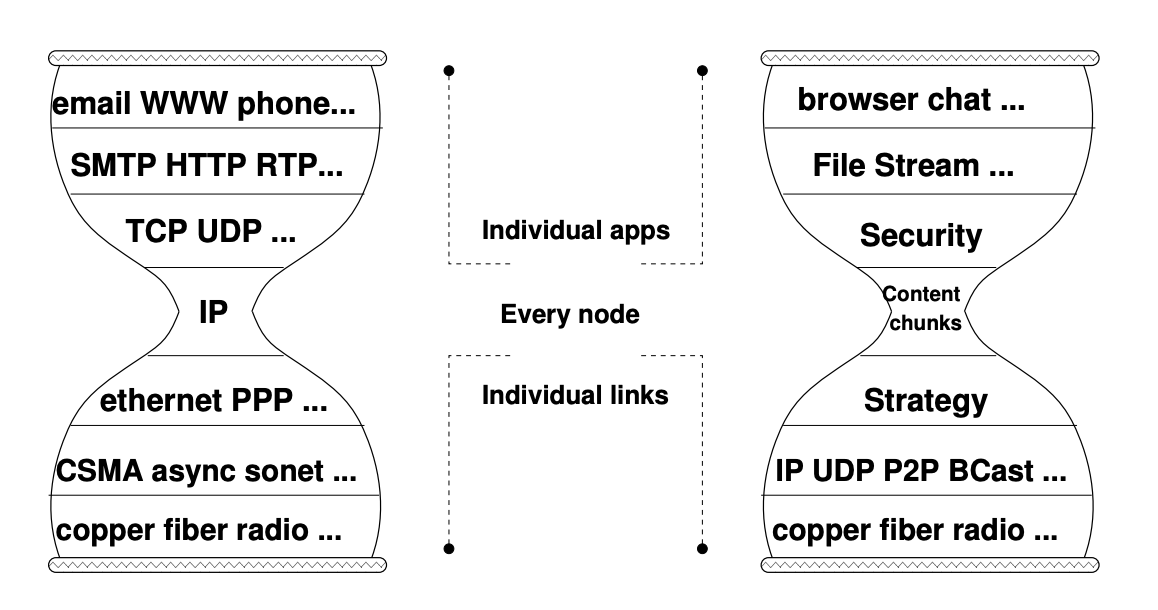
\includegraphics[height=0.5\textwidth]{img/ndn-stack.png}
	\end{minipage}}
 \hfill 	
  \subfloat[]{
	\begin{minipage}[c][1\width]{
	   0.5\textwidth}
	   \centering
	   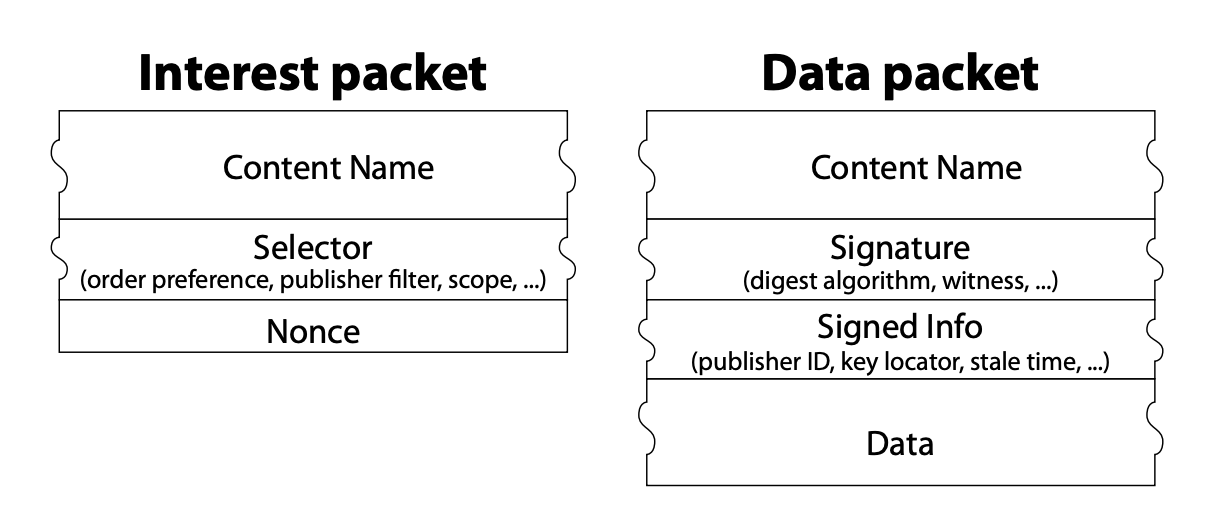
\includegraphics[height=0.5\textwidth]{img/ndn-packets.png}
	\end{minipage}}
\caption{Named Data Networking design. Source \cite{jacobson2009networking}}
\label{fig:ndn-design}
\end{figure}
NDN defines two types of packets: Interest, and Data (see Fig. \ref{fig:ndn-design}b). Interest packet as the name suggest, indicate the interest of some data chunk, where the data chunk is identified by its Content Name. An consumer broadcast a interest packet to all its connection faces. If any node which receive such message has the corresponding data locally (in Content Store), it can respond with the Data Packet. 
The operations of NDN node are similar to IP node. In Fig. \ref{ndn-operations} we can see the forward engine model in NDN node. When request arrive at one of the available faces it get dispatched based on the lookup result. 

The FIB (Forwarding
Information Base) is responsible for forwarding the interests to potential nodes where the data can be found (similar to FIB used in IP, except it allows for multiple outgoing faces rather than single one). 

The Content Store(CS) is responsible for buffering a content that was requested by Interest packet. Since the data can be served to multiple consumers–––not just single connection, as it is done in IP––it is not recycled after the first Interest request is satisfied. This mechanism is called in-network storage, because the network itself is storing the data. It is possible due to idempotency, self-identification, and self-authentication of the packets so each packet is equally useful for many consumers (e.g. two hosts interesting in Netflix video, can receive the content from single node without requesting the Netflix servers). The data is stored as long as possible and different storage policy can be used e.g. LRU replacement.

The PIT (Pending Interest Table) store information about the interests forwarded to potential data sources. When one of them reply with the Data packet, the PIT is checked if some consumer is waiting for the data, and if so, the Data packet is forwarded to corresponding face.
\begin{figure}[h]
    \centering
    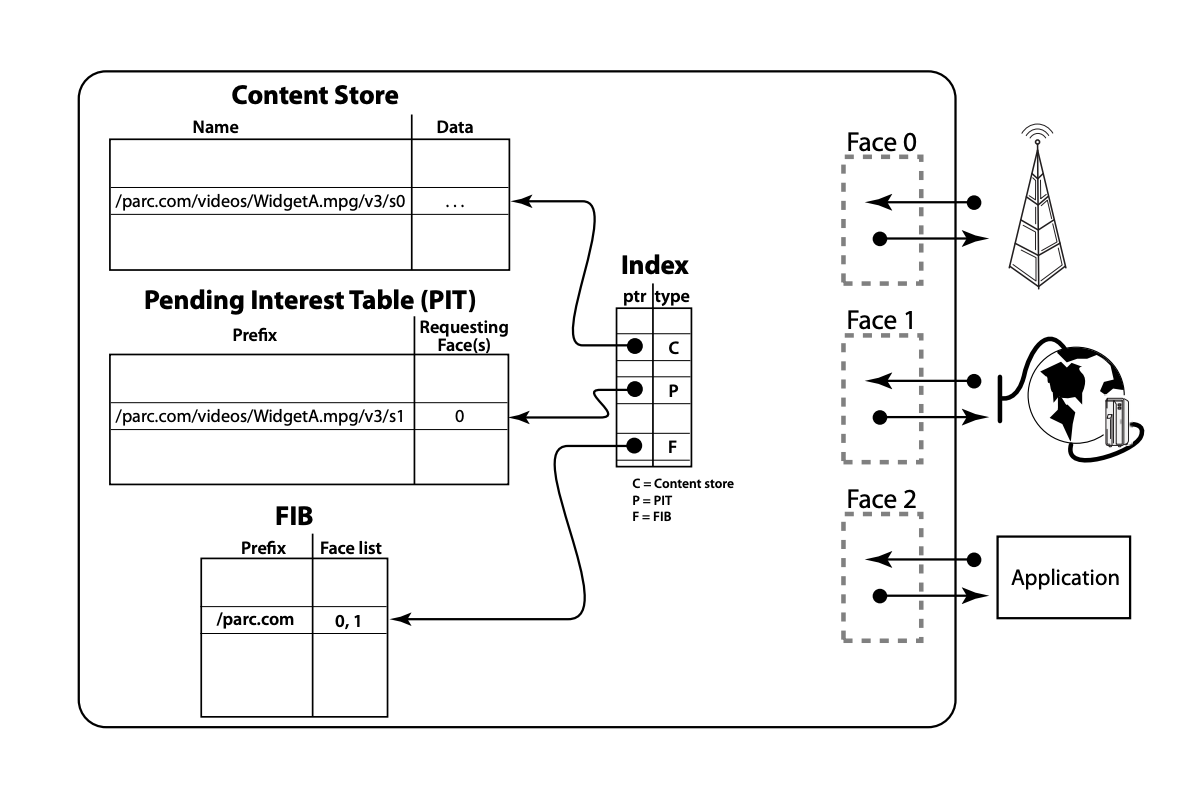
\includegraphics[width=\linewidth]{img/ndn-operations.png}
    \caption{NDN node operations. Source \cite{jacobson2009networking}}
    \label{fig:ndn-operations}
\end{figure}

To better understand the model, the concrete packet flow is presented in Fig.\ref{fig:ndn-flow}. 
\begin{enumerate}
    \item 1. The requester application wants to receive some data so it sends the request to its local NDN engine. The node first check the local CS, and since the concent is absent, it request the Interest packet to the closes router.
    \item 2. The router first check its Content Store, and if the data is absent, it check if there is already pending interest in PIT for such data, if not the request is forwarded to the next router according to FIB.  
    \item 3. The next router do the same as previous router, it check its CS, PIT, and then forward the Interest packet through FIB.
    \item 4. Finally the Interest reaches the data source router, where the content is present in the CS so it is immediately returned.
    \item 5. The router receive the Data packet and store it in its CS, check which nodes are waiting for the data in PIT and forward the Data packet accordingly.
    \item 6. This router (that was initialy requested by the requestor) do the same as the previous router storing the data in CS and responding with the Data packet.
    \item 7-8. After some time, when different requestor ask for the same data, it gets immediately response from its closes router–––saving the network bandwidth and reducing the latency.
\end{enumerate}

\begin{figure}[h]
    \centering
    \includegraphics[width=\linewidth]{img/ndn-flowoperations.png}
    \caption{NDN packets flow. Source \cite{ahlgren2012survey}}
    \label{fig:ndn-flow}
\end{figure}

%\section{IPFS}
%IPFS (Inter-planetary file system)\cite{benet2014ipfs} is a peer-to-peer distributed file system; its goal is to create a global file system where each file is indexed by its content hash. 
%In the traditional web, we request file by its URI - which then resolves to a certain location where the content is hosted. In IPFS we request a file by its content hash - which then resolves to the closest location where the file can be accessed; it can be either: cache, local storage, our neighbor, our ISP node, any other peer in the network, or finally the content publisher. This is possible not because of the structure of the network, but because we request the content. In the traditional web, each time we request the URI it can resolve to different content, therefore we can not trust our neighbor, that he will send us the content we were asking for. 
%Additionally, in IPFS, each content is signed by its publisher keypair, so we can be sure that the content that our neighbor is serving us, is the thing that was created by the publisher. Therefore if we request a malicious link (hash of the content) and it's integral with its content, we still can reject it -- if it's not signed by the actual publisher we are interested in. 
%We can state that IPFS natively guarantees integrity and authentication.

%The fact that the content is authenticated by the publisher keypair seems to be perfectly fine. But here in this thesis, we double down on possible threats and propose solutions on how to solve them.

\chapter{Content Poisoning}
\label{content-poisoning}
First, we narrow the area of research in this thesis. Content Poisoning in NDN (and possibly in all ICN networks) can be divided into two categories: 1. Corrupted Data, and 2. Fake Data. In both of them, content gets modified. The first one assumes that an attacker does not possess a signing-key of an authentic publisher; thus, the content will not pass a signature verification process. It might look like the problem is resolved. Unfortunately, signature verification is an optional process, and there are two reasons why this process might not be done on every router. The first one is economic incentivization. The process of signature verification is resource-consuming; thus, businesses might decide to skip it. The other reason is that a signature verification requires a corresponding public key. We cannot expect from router to store all possible public keys. Thus the routers are vulnerable to Corrupted Data CPA. This kind of attacks has been addressed in papers \cite{ghali2014needle} \cite{yu2018content} \cite{nguyen2017content}. 

The second CPA category––Fake Data––is more dangerous because it assumes that an attacker gets access to the publisher's private key. Therefore he can forge a valid signature, which will successfully pass verification on an end-system. 

Once a bogus content gets propagated across multiple nodes (more specifically on their Content Stores), each end-user who requests content from that node receives the poisoned content. Signature verification passes successfully; hence a user is convinced that the content is authentic. Moreover, the content cannot be as easily revoked as it was disseminated because most ICN networks do not allow removing/revoking its cache content, other than natural (e.g., LRU based) cache aging. The one way to effectively prevent fetching fake content is by explicitly filtering the name of the content we consider poisoned. However, this raises another problem, how a user can know the name of the poisoned content, and if it is not too late. In \cite{nguyen2017content}, we can read, "Therefore, it (Fake Data CPA) is harder to create but impossible to detect by end-systems." At the time of writing, the problem is still unsolved, but there is one proposal \cite{konorski2019mitigating} which we research, expand, and modify. Before that, we will briefly review how other content-oriented services solve the Fake Data CPA problem.

\section{Wikipedia}
Wikipedia is an example of a system that faces a content poisoning problem. Let us investigate how do they solve the problem. 

"Wikipedia is a free online encyclopedia, created and edited by volunteers around the world and hosted by the Wikimedia Foundation."
Everyone can become a Wikipedia editor just by creating a free account. Account registration does not even require an email address. An editor can create a new article or modify an existing one. Before a change is publicly available, other editors read the proposition and have a chance to reject it or propose a further edit. If they cannot achieve consensus, they start a discussion and exchange their arguments. Finally, if they agree on one version, a consensus is achieved, and the new version of an article is published (keeping the whole history of changes).
Such ease of account creation makes Wikipedia vulnerable to Sockpuppeting (also known as Sybil attack). This vulnerability allows one user to create multiple accounts with different identities. Consequently, one person controls fake "public opinion," which can support his position in edits discussions. That is why a raw voting system is a non-preferred method in conflict resolutions.
Wikipedia fights content poisoning attacks by using humans to detect bogus changes. This mechanism seems to work well in such a service, but it does not scale to a public Internet protocol, so cannot be used as is.

\section{LOCKSS}
LOCKSS is a decentralized p2p digital preservation system for libraries, developed at the Standford University \cite{maniatis2003preserving}. Currently, it is an open-source, decentralized system used by many institutions. It is helping them to maintain a digital collection of journals, articles, and books. If we abstract from a specific type of data the system is operating on, we notice some similarities with ICN networks that we believe are worth investigating. The main difference between LOCKSS and ICN is that the former is very conservative; it rather prevents than expedites change of data. Nevertheless, this property may be useful in the context of preventing bogus data diffusion. 
In LOCKSS, each participating library becomes a node in a p2p network. It runs software responsible for collecting new content from e-journal websites by a crawler, serving already stored materials to local readers, and cooperating with other nodes in preserving materials when they get damaged. 
Due to publishers' copyrights, no node has to redistribute its content blindly to other peers. Other nodes can help repair damaged or completely missed material only to nodes that previously proved its ownership. New materials can only be acquired directly from a publisher's website to libraries which paid for subscription. 
Cyclic polls detect damages. Each interested peer votes on a hash of an Archive Unit (AU), the smallest unit in which nodes identify content. Since each node consists of a different set of Archive Units, the protocol treats each AU independently. If it turns out that some node contains AU with a different hash than most of the poll, it starts a sequence of repairs. As a result, LOCKSS becomes a self-healing store of data and does not increase the risk of free-loading non-purchased content.
LOCKSS is designed in a way that does not rely on long-time public-key cryptography (a system that must operate for decades is eventually highly susceptible to private-key leakage). Since it does not rely on public-key cryptography, peer identity management is minimalist; therefore, such a system cannot rely on peer reputations.

\section{Social Media and Fake News}
Fake News is deliberate disinformative news that is hard to identify and can lead to destructive consequences if not mitigated in time. Social media are a perfect ecosystem for disseminating fake news; specially designed algorithms serve us content that we are likely to agree with. In \cite{zhou2018fake}, the authors point out why social media algorithms are very effective in fake news dissemination. Social media allow us to form like-minded people into groups more accessible than ever before. Such groups facilitate the Echo Chamber Effect, where each individual is surrounded by people who share and produce content that fits our current worldview. It leads to a segmented and polarized society, which is very prone to believing fake news that confirms current opinions, even if there is limited or no reason to believe it. 

Fake news is often written in a very provocative fashion, making such content more attractive for interaction; more interaction leads to higher dissemination, fostering even more interaction. While for honest publishers and valuable content, this feature is helpful, it becomes a hazardous tool in the hands of malicious publishers. Additionally, the low cost of creating new accounts makes it even easier for an attacker to initiate the snowball effect, using fake accounts. Bots can interact with people or even with other bots, creating fake social opinions.  

We notice that this model fits perfectly into our Content Poisoning Attack model. In some sense, we are facing a similar problem fake news does in social media: we want to allow valuable content to spread as fast as possible, while limiting malicious content dissemination to a minimum.


\subsection{Mitigating fake news}
\label{mitigating-certification-services}
One idea is to create centralized services that reveal known fake news. Each time someone is susceptible to some news, they can check if the news is not present in blacklisted news. This solution has some flaws. Attackers can publish honest news in such an "oracle" service, leading to revoking genuine news, which can be as harmful as publishing fake news. A better way would be to check many independent "oracle" services and arrive at a decision whether to believe based on how many of them are skeptical of such news.

Another idea would be to create certification services. Each news could be signed by services that decide which content is authentic. A user could decide which certification services he/she trusts, and therefore inherit the trust in the news signed by such services. This idea seems to have worked for decades in journalism. A reliable journal reader does not need to check each article if it is fake or not. He inherits each article's confidence because he trusts that the journal's reviewers have eliminated fake or low-quality content. Additionally, a journal publisher has no interest in publishing low-quality content because he/she has economic incentives to become as creditworthy a publisher as possible.
This idea has some downsides. The process of reviewing an article is prolonged and requires qualified human interaction. Although some of the work can be outsourced to artificial intelligence, it is still a complicated task. Additionally, a journal publisher can introduce censorship or favor some kind of content. In other words, this mechanism does not scale for general-purpose content certification.

Let us consider fake news detection in practice. If Alice forgets to log out from social media account on a public library computer, someone can submit content, a post, that says, "I do not want to live anymore the way everyone else is living, this rat race is not for me, from today I become homeless. Goodbye." Such content is an excellent candidate to become successful fake news mainly because it is created from an author's account, which gives it high credibility, but also because it contains some arguable truth that can make it trustworthy. Unfortunately, as we discussed in the previous certification services approach, this idea of content evaluation does not scale to the level we need. We notice that to decide if a post is fake or not, we can just wait. In this situation, the time is playing a crucial role, because if the post is deleted from Alice's account after a short period, we can be sure that Alice would never have posted it. On the other hand, if the post is present for a long time on her page, we can state with high probability that she wants it to be there, thus it is authentic content.

This approach also has its downsides, namely, it is slow. If a piece of information is urgent, like information that some country has started World War III, we do not have hours to wait until the information gets deleted or not. We need to act fast. In such situations, this approach is inefficient. But for less urgent content, this approach offers several useful features. It scales well--for each content publication, only one person is involved to remove the content (in the case when it is bogus). It is maintenance-free--by default, no one needs to do anything if the content is authentic. It is flexible--a reader can individually decide if the time from publication is long enough to trust such content or not. If the information is not very impactful, we can trust it from the first hour from the publication; otherwise, e.g., in the case of a banking webpage, we could wait a few hours until we enter the credentials into it. It is like HTTPS and HTTP, but much more flexible--some pages can be safely browsed over HTTP, while others should be used only over HTTPS. 

As discussed before, the fake news problem in a social network is very similar to the CPA problem in ICN networks. So the solutions that work in one domain could work in the other. In this thesis, we will continue the idea of a content time availability, which we will call \emph{Proof-of-Time}.
\chapter{Proof of Time}
\label{proof-of-time}
In the previous chapter, we introduced a mechanism for mitigating fake news propagation on social media accounts based on waiting––in the hope that bogus content will finally be removed, distinguishing it from authentic one. In this chapter, we generalize the mechanism to solve the CPA problem in ICN networks. Before that, we make some assumptions. First of all, an attacker is operating in a time constrained environment. He/she eventually loses access to stolen credentials, either by revoking, expiring, or any other external factor. Additionally, he/she is unable to refresh the credentials infinitely long. As a result, his/her access (measured in time) to a publisher's account is limited, in contrast with real account owners whose access is unrestricted.
We leverage the difference between those two scenarios to create a new method of authentication. This method requires each publisher to prove access to credentials over some period of time, hence the name \textit{Proof of Time}.

If a traditional model of authentication is based on proving access to credentials associated with an identity, then we can write
\[access\ to\ credentials \implies authenticity\].
In this thesis, we extend this model to access to credentials over some period of time. We write
\[access\ to\ credentials \land access\ to\ time \implies authenticity\]

In the previous section, we discussed how the mechanism could work in social media networks. ICN networks are different in that they do not allow to remove content because it is distributed across many routers within their data cache (Content Store), to ease content dissemination. To support content removal, each node would need to periodically ask a publisher if the content has been removed or not, in In this way, sacrificing scalability, which was the reason the ICN was created in the first place. 
Instead of requiring a publisher to remove content, we create an overlay network of trust, where trust in content serves as a primitive. When the trust is low, a user should be discouraged from using the content (similar to how modern web browsers discourage usage of the insecure HTTP protocol). 

In such an overlay trust network, each piece of content has its Credibility Score. The Credibility Score is gained by proving access to credentials over some period of time. In other words, the longer a publisher is able to sign content, the higher is the Credibility Score for the content. With that model, we can assume that a malicious actor is unable to achieve enough Credibility Score to convince a network about its trustworthiness, while a legitimate publisher will eventually achieve it over time. Later on we will discuss how to design such an overlay network in order to accomplish such an authentication mechanism.

\chapter{Network structure}
\label{network-structure}
In the previous chapter, we mentioned the need to create an overlay network of trust where each publisher tries to convince the rest of the network about its trustworthiness by increasing the Credibility Score of the published content. In this chapter, we will discuss the considered network in more detail. 

\section{Trust propagation}

As discussed before, the Credibility Score will spread across the ICN network nodes. It can spread in various ways, and in this chapter we will explore different models for this kind of mechanism. 

One proposal\cite{konorski2019mitigating} abstracts the concept of trust to the concept of infection and so allow us to adopt the knowledge created by biological research. In our case, each node that develops trust in some content is called infected. Each node that does not trust the content is called healthy. By default, all nodes are healthy; therefore, no one trusts the content.
A publisher can infect nodes by sending them a proof-of-time certificate.
Each node that gets the certificate sets a Credibility Score to 1 in its local trust table. In this way, the publisher can quickly flood the whole network, which leads to an epidemic in a relatively short time. However, we need trust to increase slowly enough for a malicious publisher to be unable to infect the whole network. 

To slow down the spreading process, we can use various mechanisms. In \cite{konorski2019mitigating}, the author proposed a mechanism where each node refuses to get infected unless the previous node signs a certificate. In this way, the publisher has to infect new nodes sequentially, much slower than infecting them in parallel. To control the speed of infection dissemination we can design nodes to sign the certificate after some (e.g., 10-minute) delay. It might be the analog to the time when a host is infected, but is not infecting other people yet. This constraint seems to prevent rapid dissemination, but a smart publisher could request many nodes at a time to sign the certificate and conduct many chains of certification in parallel. To prevent that, we need to force the publisher to start a certification chain from his/her home node assigned by some external mechanism, and each node needs to indicate which node is the next to trust the certificate. In this way, the publisher can not create the certification chain in parallel; it needs to instill infections in a succession. This mechanism is similar to the iterative DNS query; see Fig. \ref{fig:iterative-publications}.

\begin{figure}[h!]
    \centering
    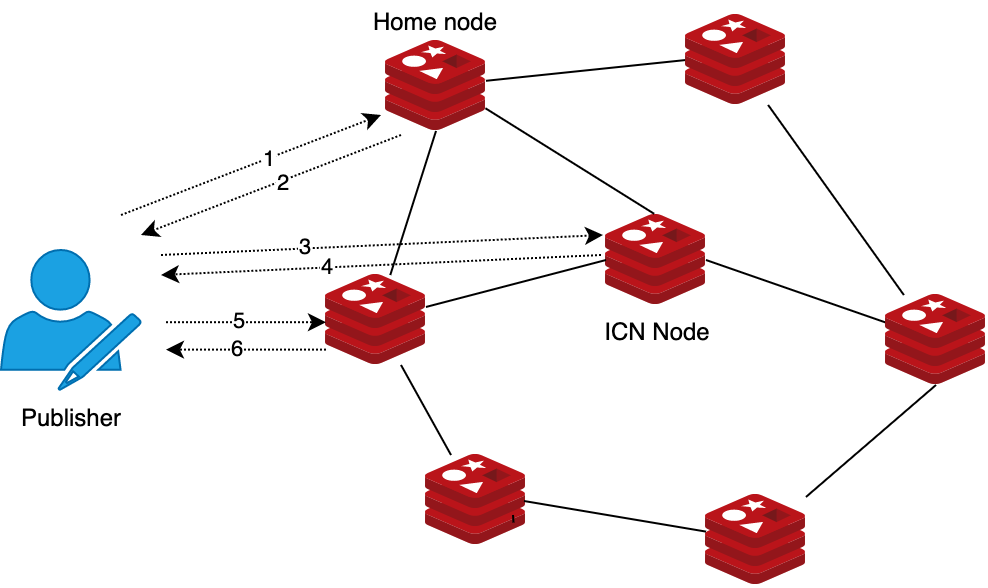
\includegraphics[width=\linewidth]{img/iterative-publications.png}
    \caption{Iterative publications of proof-of-time}
    \label{fig:iterative-publications}
\end{figure}

There are still some missing points that we need to solve. Although we can control infection dissemination speed, we do not have a mechanism to recover from malicious publications.  After a limited period of time the network should eventually notice the malicious publisher and reject the authentication. At the same time, an honest publisher who does not have time constraints can successfully infect the whole network––causing an epidemic and thus authenticating the content. 

We therefore need to add a node recovery mechanism. Once the node is infected, it should remain so for a limited period of time. After that time, it recovers, becoming healthy, i.e., distrusts the content. The period of time needs to be carefully designed so the nodes do not recover too fast because it would lead to the nodes getting infected slower than they are recovering. 

The requirement that the nodes be infected in succession is inconvenient. It would be much better if, following a limited succession of infections, another mechanism could infect the rest of the network.
For that, we can use an additional mechanism for inner infections. Each node gets infected not only by a publisher certificate, but also by the neighbor nodes. In this way, the publisher would be responsible just for starting the initial infection succession, which should embrace the whole network if it is long enough. 
\chapter{Epidemiology}
\label{epidemiology}
To get some background for the graph infection algorithm, we first outline infection processes in the field of epidemiology.

In epidemiology there exist models that represent a spread of disease, such as SI, SIR, SIS, SIRS. Each letter designates the possible state an individual (host or node) can be in, respectively S - susceptible, I - infected, R - recovered. An individual in the S state is healthy, but can contract a disease in contact with someone infected; in the I state is infected and can infect others, and in the R state has recovered. Although this classification is simplified and does not consider inner body mechanisms, it is enough to observe what is happening on a network level. Additionally, the above models entirely ignore contact networks, assuming that each individual has an equal chance to contact anyone else in a unit of time, a so-called \textit{homogeneous mixing} assumption.

\section{SI Model}
SI is the simplest and most primitive model, assuming that there are only two states of a node, susceptible and infected. Let $S(t)$ be the number of nodes in the S state at time $t$, and $I(t)$ be the number of nodes in the I state. Since the disease-spreading model is a random one, those numbers are not deterministic and can vary among instances of the infection process, even in the same conditions. To get around this problem, we will treat $S$ and $I$ as the average number of susceptible or infected nodes over many instances with identical conditions.
In this model, we allow only one kind of state transition, from S to I — the state changes when a susceptible individual meets an infected one. If the total population consists of $n = I + S$ people, then the average probability of meeting a person in a susceptible state is $\frac{S}{n}$.
Let $\beta$ be the chance that individuals contact someone else in a unit of time. 
Hence an individual has a $\beta*\frac{S}{n}$ chance of contact with a susceptible individual.
Since the total number of infected people is $I$, then the rate of new infections per unit of time is equal to $I * \beta*\frac{S}{n}$.

The SI model can be written as an ordinary differential equation (ODE):
\begin{equation} \label{si_ode_i}
\frac{I}{dt} = I \beta \frac{S}{n}
\end{equation}
Accordingly, the decreasing rate of susceptible equals:
\begin{equation} \label{si_ode_s}
\frac{S}{dt} = -I \beta \frac{S}{n}
\end{equation}
We can also rewrite the equation to the variables representing fractions of susceptible and infected nodes
\begin{equation}
s = \frac{S}{n}, i = \frac{I}{n}
\end{equation}
Then we can rewrite Eqs. \ref{si_ode_i} and \ref{si_ode_s} as:
\begin{equation}
\begin{split}
\frac{di}{dt} &= i \beta s \\
\frac{ds}{dt} &= -i \beta s
\end{split}
\end{equation}

This kind of differential equations are called logistic growth equations, and can be solved with:
\begin{equation}
\begin{split}
i(t) =\frac{ i_0 * e^{\beta*t} }{(1 - i_0) + i_0 * e^{\beta*t}}
\end{split}
\end{equation}
Wwhere $i_0$ is the value of $i$ at $t = 0$. In Fig. \ref{fig:logistic_growth} we see the $i(t)$ function where $i_0 = 0.01$, $\beta = 1$.

\begin{figure}[h!]
    \centering
    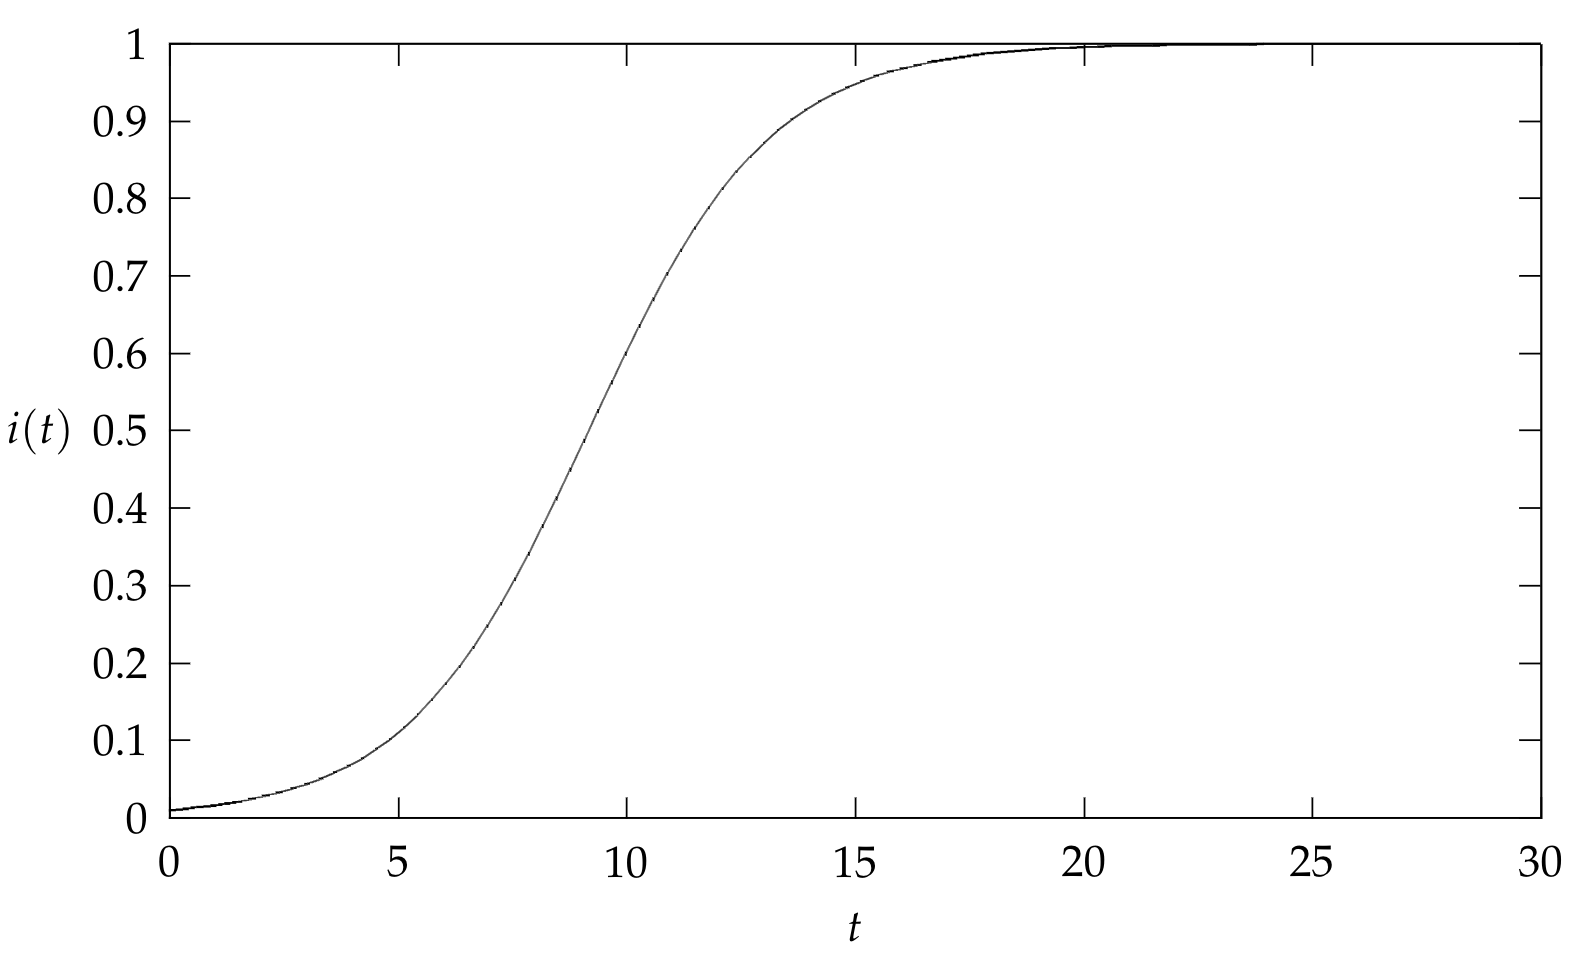
\includegraphics[height=6cm]{img/logistic_growth.png}
    \caption{Logistic growth function $i(t)$}
    \label{fig:logistic_growth}
\end{figure}

\section{SIR Model}

SIR model introduces the R state to the SI model. When, in the SI model, an individual gets infected, it remains so forever. SIR model allows infected nodes to recover from the disease after some time. In the real world, this might be because of the immune system fighting the disease. Additionally, once an individual recovers from the infection, it becomes immune to further infections. Therefore in SIR, an individual can change state only from S to I to R. In this mathematical model, we do not distinguish if the R state is obtained by immunization or death, since in both cases, an individual is removed from the potential disease hosts pool. Because of that, the model is also called susceptible-infected-removed.

Call $\gamma$ the chance of recovering from the I state. Then the ODE system for SIR model becomes:
\begin{equation}
\begin{split}
\frac{ds}{dt} &= -\beta i s \\
\frac{di}{dt} &= i \beta s - \gamma i \\
\frac{dr}{dt} &= \gamma i
\end{split}
\end{equation}

To see how this model behaves with some concrete values, consider the COVID-19 epidemic with the following assumptions: three individuals were initially infected at $t_0$, the total human population is 7.8b people, and no individual was immune to the disease at $t_0$. Hence,
\begin{align*}
I(0) &= 3 \\
S(0) &= 7.8 * 10^9 \\
R(0) &= 0
\end{align*}

We assume that each infected individual, on average, makes a possibly infecting contact once in two days (assuming homogeneous mixing across the whole globe), and the infection duration is five days: 

\begin{align*}
\beta &= \frac{1}{2} \\
\gamma &= \frac{1}{5}
\end{align*}

The following plot (Fig. \ref{fig:covid1}) shows fractions of susceptible, infectious, recovered individuals in the whole population as a function of time.

\begin{figure}[ht]
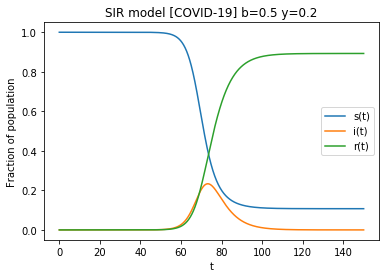
\includegraphics[width=9cm]{img/covidb12y15.png}
\centering
\caption{COVID-19 in SIR Model for $\beta=0.5$}
\label{fig:covid1}
\end{figure} 


If we decrease the number of infections to one in five days, so $\beta = 0.2$, then there is no epidemic (see Fig. \ref{fig:covid3}).

\begin{figure}[ht]
    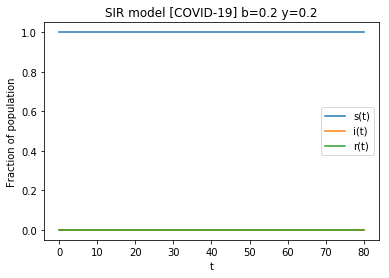
\includegraphics[width=9cm]{img/covidb15y15.png}
    \centering
    \caption{COVID-19 in SIR Model for $\beta=0.2$}
    \label{fig:covid3}
\end{figure} 

The rate of new infections $\frac{di}{dt}$ determines if an epidemic will happen; if it is positive, then there will be an epidemic, and if it is negative, individuals will recover faster than the spread of infection, so there will be no epidemic.

We can calculate the value of $\frac{di}{dt}$ at $t_0$ and check if the value is negative or positive; the negative value means the decrease of infections from the beginning, so we can be sure that eventually there will be no infections.

The condition determining if an epidemic will happen or not,is thus
\begin{equation}
i \beta s_0 - \gamma i > 0
\end{equation}
Since the fraction of infections $i$ is never negative, we can omit it to get
\begin{equation}
s_0 > \frac{\gamma}{\beta}
\end{equation}
We can introduce $R_0$, the Basic Reproduction Number:
\begin{equation}
R_0 = \frac{s_0 \beta}{\gamma}
\end{equation}
which represents the number of individuals that each infected individual can infect before recovering. Thus if $R_0 = 2$ then each infected individual can infect on average two other individual before recovering, so the number of infections grows exponentially, and if $R_0 = 0.5$, then for every two individuals, only one new infection happens, and the number of infections decreases exponentially. $R_0 = 1$ is called the \textit{epidemic threshold}, where the number of new infections equals the number of recoveries, so the total number of infected individuals is always the same and equals the initial number of infected individual $I_0$. 

For example, for seasonal flu the value of $R_0$ is estimated between 0.9–2.1 \cite{coburn2009modeling}, whereas for COVID-19 it's estimated to 2.2 in early-stage (January) \cite{li2020early} and recently to 5.7 (April) \cite{readeid}.

To mitigate an epidemic, we can decrease $s_0$ and $\beta$, or increase $\gamma$. Since we have little control over the time of recovery ($\gamma$), the only way to reduce the impact of infection is to reduce the number of contacts between infected and susceptible individuals (which is why social distancing is so crucial in a fight with epidemics).


\section{SIS Model}
There are some diseases where an individual can get infected many times, e.g., the flu. Therefore there is no Recovered population. This could be because the virus is mutating, or antibodies do not persist long enough in the organism. For this kind of epidemic, the state flow is $Susceptible → Infected → $Susceptible, hence the name SIS. 
For this kind of model, we need to modify the previous equations, so that the fraction $\gamma i$ will go to the S state, instead of the R state.
\begin{equation}
\begin{split} \label{eq_sis}
\frac{ds}{dt} &= - i \beta s + \gamma i \\
\frac{di}{dt} &= i \beta s - \gamma i
\end{split}
\end{equation}


We can solve the equations by substituting $s$ in the second equation and solving a Linear Differential Equation:
\begin{equation}
\frac{di}{dt} = i * \beta * (1 - i) - \gamma * i
\end{equation}
After integrating we get:
\begin{equation}
i = (1 - \frac{\gamma}{\beta}) \frac{C}{C + e^{-(\beta - \gamma)t}}
\end{equation}
where 

\begin{equation}
C = \frac{\beta i_0}{\beta-\gamma-\beta i_0}
\end{equation}
In Fig. \ref{fig:sis_it} we can see a plot of the function $i(t)$ for constant $\gamma = 0.2$ and $\beta = 0.5$.

\begin{figure}[h!]
    \centering
    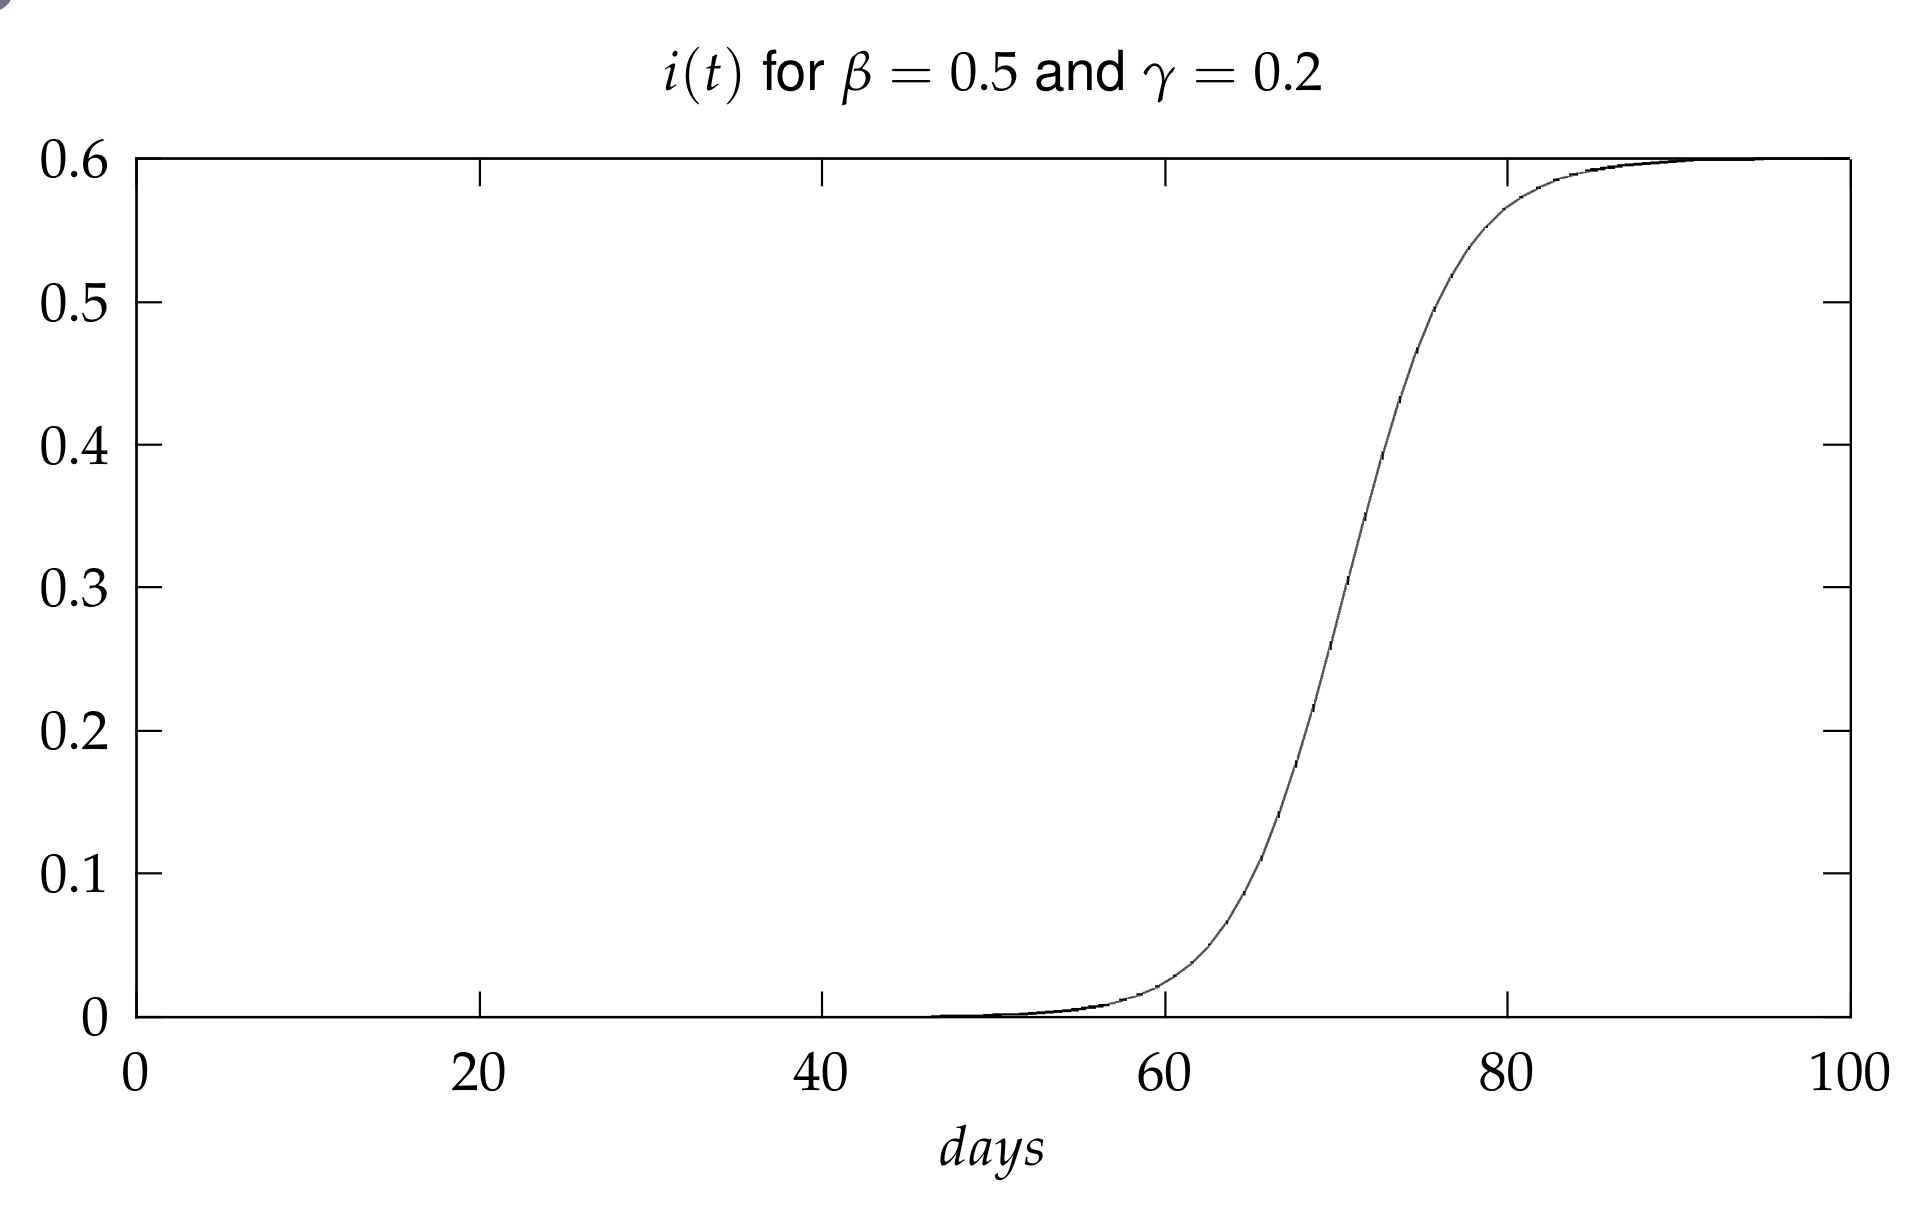
\includegraphics[height=7cm]{img/sis_it.png}
    \caption{$i(t)$ for $\beta = 0.5$ and $\gamma=0.2$}
    \label{fig:sis_it}
\end{figure}

Also, in Fig. \ref{fig:sis_ibt} we plot the function $i(t, \beta)$ for constant $\gamma = 0.2$ to see how the $\beta$ influences the results.
\begin{figure}[h!]
    \centering
    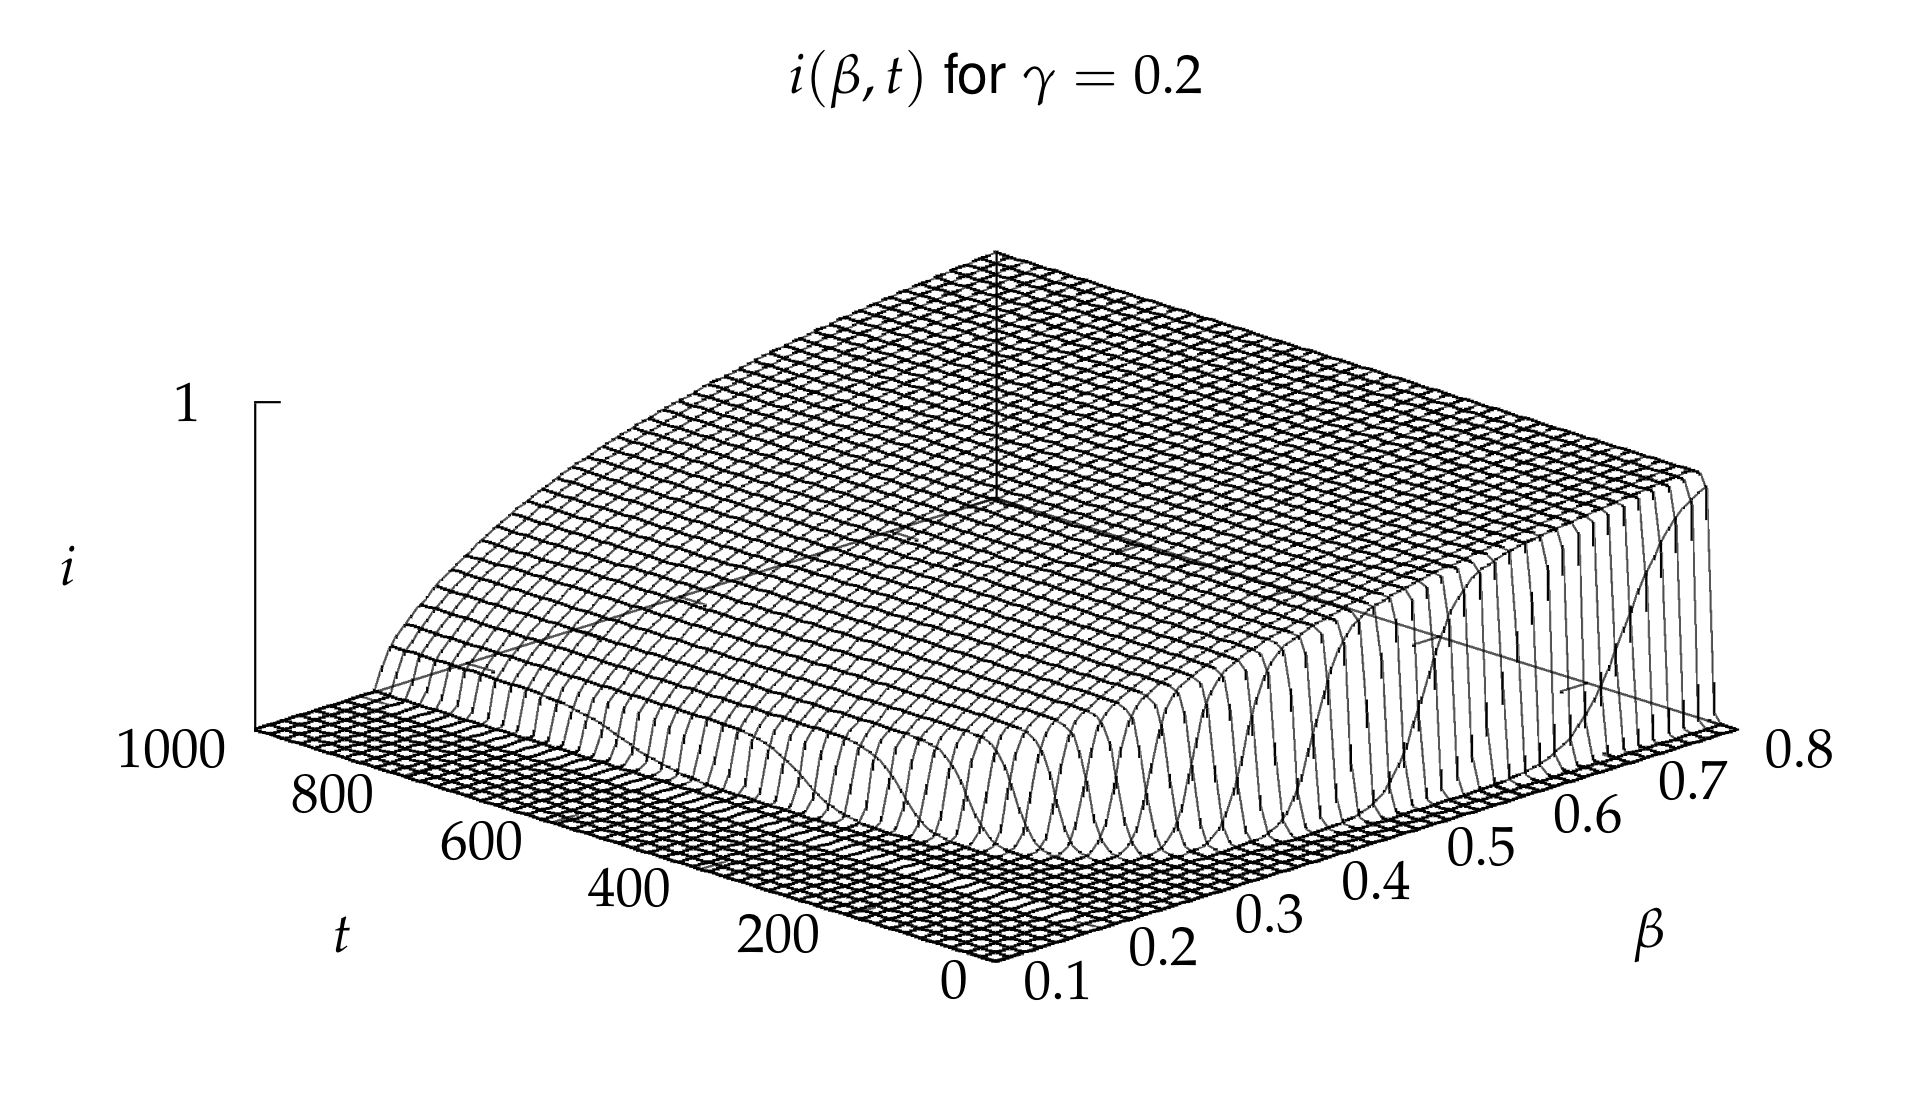
\includegraphics[width=\textwidth]{img/sis_ibt.png}
    \caption{$i(\beta,t)$ for $\gamma=0.2$}
    \label{fig:sis_ibt}
\end{figure}
As we can see, it drives the number of the infected population. If it is less than $\gamma$, the epidemic never occurs. Values greater than $\gamma$ lead to a constant fraction of the infectious population (the rate of catching the infection by the susceptible population is equal to the rate of recoveries in the infected population). The higher the $\beta$, the faster is the outbreak, and the higher the infection ratio.

\section{SIRS and SEIRS Models}
SIRS model introduces another state change, allowing recovered individuals to lose their immunity. Therefore the state flow is: $Susceptible → Infected → Recovered → Susceptible$. We can write equations for this model by simply adding one intermediate state equation to Eq. \ref{eq_sis}.
\begin{equation}
\begin{split} \label{eq_sirs}
\frac{ds}{dt} &= \delta r - i \beta s \\
\frac{di}{dt} &= i \beta s - \gamma i \\
\frac{dr}{dt} &= \gamma i - \delta r
\end{split}
\end{equation}

Another, more complex model in terms of the number of states is the SEIRS model. This model introduces an intermediary Exposed (E) state between the S and I states, where an individual is infected but does not spread infection to other people. Such modification is also easy to write by adding another intermediary state to Eq. \ref{eq_sirs}.

\begin{equation}
\begin{split}
\frac{si}{dt} &= \delta r - i \beta s \\
\frac{ei}{dt} &= i \beta s - \gamma e \\
\frac{di}{dt} &= \gamma e - \omega i \\
\frac{dr}{dt} &= \omega i - \delta r
\end{split}
\end{equation}


Clearly, these models can be easily extended to an infinite number of intermediary states, more accurately reflecting reality. Unfortunately, there is no known analytical solution to such models; they have to be solved by numerical integration of differential equations.

\section{Summary}
The above outlined models hinge on the idealistic full-mixing assumption, where each individual has an equal probability of contacting anyone else. This assumption does not reflect precisely human interaction or distributed computer networks. The $\beta$  parameter reflects a chance of an individual to contact someone else and spread the infection. In our problem, the network is static, the structure of nodes is fixed; each node has a unique set of neighbors through which the disease can spread. In real life, this might be family members, friends, or coworkers. The chance of contact with the rest of the population, like the chance of meeting two people from two ends of the earth, is minimal. For this reason, we have to consider a different model of infection dissemination. 
In our model, the infection is an abstract representing trust in content. We will look at how trust graphs are built to understand how to leverage the above mechanisms for our infection spreading model.
\chapter{Trust graph}
\label{trust-graph}

People are still one of the most advanced technology. We can get inspired by some of the solutions that work in human societies for centuries.
Yuval Noah Harari in his book "Sapiens: A Brief History of Humankind" \cite{harari2014sapiens} states that the most important feature of human language is a rumor. Rumor let us know which person is not trustworthy without having to interact with him directly. If our best friend Bob, tells us, that Carlie is theft, we do not need to get stolen to be convinced about it. The same applies to an inverse scenario, if Bob tells us, that Carlie sells great quality products, we are now more likely to buy products from him; we are biased towards people, whom we get positive rumors. We notice that each person we know directly or indirectly gets labeled with some tags. One can be labeled as Helpful, Conscientiousness, and also Not-Trustworthy, while others can be labeled as Unhelpful, Lazy but Trustworthy. Here in this thesis, we are limiting our range of study just to the dimension of Trustworthiness.
If we have three friends Alice, Bob, Charlie. Alice and  Bob tell us that David is Trustworthy, while Charlie claims that he is not. The decision to labeling David as Trustworthy or Not-Trustworthy, requires some kind of decision evaluation algorithm.
One might assume that if there is at least one person who does not trust him, there must be something wrong with him, and will label him as Not-Trustworthy. One can use another evaluator which says, do want the majority of people do, thus if Charlie is trusted by the majority, I will trust her too. Another one can slightly generalize this evaluator and say that person is trustworthy, only if $\xi$ percentage of my friends trust him. 

At this point, it is worth introducing some conventions. When we say friend we mean a trustworthy person, in other words, a person whom we have trust relation to. Let $N$ be a set of all considered individuals. Let $F_n \subset N$ be a set of all $n$'s friends $f \in F$. Then we call 
\begin{equation}
\%(n_1, n_2) = \frac{|F_{n_1} \cap F_{n_2}|}{|F_{n_1}|}    
\end{equation}
the proportion of $n_1$ friends who are also $n_2$ friends. Let's call $\xi$ (where $0 \le \xi \leq 1$) the minimum proportion of $n$'s friends needed to make trust relation other person in a graph. $\%_n$ who needs to trust person $n$ to make me trust him. 

Going back to our example, we trust David only if majority of our friends trust him. We denote trust function as $T : N \rightarrow \{true, false\}$, $T(n) = \%_n > \xi$. 
Let's use this formula to evaluate if $David$ is a trustworthy person. Let $\xi = 0.5$. We know that Alice and Bob do trust David, while Charlie does not.
\begin{equation}
\begin{split}
T(David) &= \%_{David} > \xi \\
&= \frac{|F_n|}{|F|} > \xi \\
&= \frac{2}{3} > \frac{1}{2}
\end{split}
\end{equation}
Then $David$ is \textbf{Trustworthy}


People with low $\xi$ easily get manipulated, we call them naive.
People with high $\xi$ hardly gets convinced, we call them stubborn. 

Another generalization might be adding weights to this evaluator, let's say that Charlie is our brother, while Alice and Bob are our cousins, and we trust 3 times stronger to our brother than a cousin. Let's call $W : F \rightarrow \mathbb{N}$ the function that maps our friend to the weight of how strong we trust him. In this case weighted proportion of our friends 
\begin{equation}
\%_n = \frac{\sum\limits_{f \in F_n} W(f)}{\sum\limits_{f \in F} W(f)}
\end{equation}

When we assume weights $W(Alice) = 1, W(Bob) = 1, W(Charlie) = 3$, and $\xi = 0.5$. We can calculate weighted proportion $T(David)$ as follows:
\begin{equation}
\begin{split}
T(David) &= \%_n > \xi \\
&= \frac{1+1}{1+1+3} > \frac{1}{2} \\
&= \frac{2}{5} > \frac{1}{2}
\end{split}
\end{equation}
Then $David$ is \textbf{Not-Trustworthy}

Another thing we can observe in the context of the trust-network is time. Should we still trust our friend from elementary school if we haven't seen him for decades? We could modify the trust function to be dependent on the time, but for now, let's assume that the friendship is immortal.

Next, if we have a friend, who has a friend, we trust that person, but he will not become our friend. If someone else ask us if he should trust that person, we would say no, because we don't want to take responsibility for people who are not our friends. Therefore only the friendship relation can propagate the trust.

Having that trust network model, we can use it to generate graphs, which then can be used to simulate infection processes. 

Having that trust model, let's describe the algorithm to generate trust graphs.
We start with a $N_0$ nodes that get connected with random $E_0$ edges, in such a way that the graph is connected. Next, for each remaining node $n \in N \setminus N_0$, we connect it to one randomly selected node in current graph. When all nodes are added, for each node $n \in N$ for each node $f \in F_n$, for each node $p \in F_f \setminus F_n$ we apply $T(n, f, p)$ function, which if evaluated to true create connection between $n$ and $p$.

In Fig \ref{fig:trustgraph500} we can see the resulting trust graph for 500 nodes and $\xi = 0.5$, and its corresponding histogram in \ref{fig:trustgraph500histogram}

\begin{figure}[h!]
    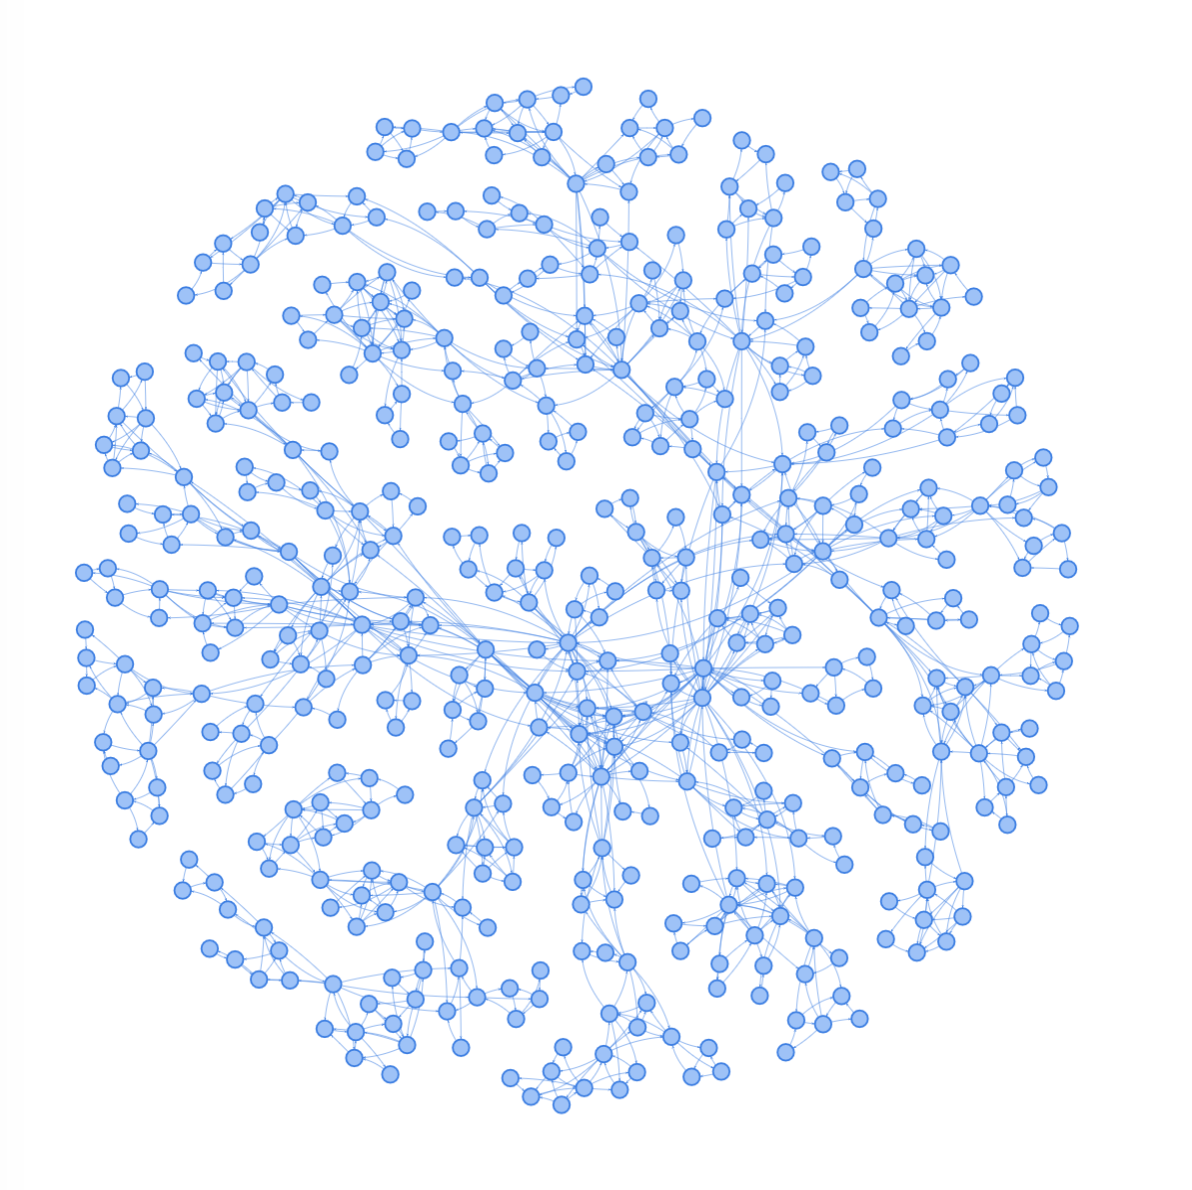
\includegraphics[width=\textwidth]{img/webOfTrust500Graph.png}
    \centering
    \caption{Trust Graph generated by Web Of Trust algorithm for $\xi=0.5$ and $n = 500$}
    \label{fig:trustgraph500}
\end{figure}

\begin{figure}[h!]
    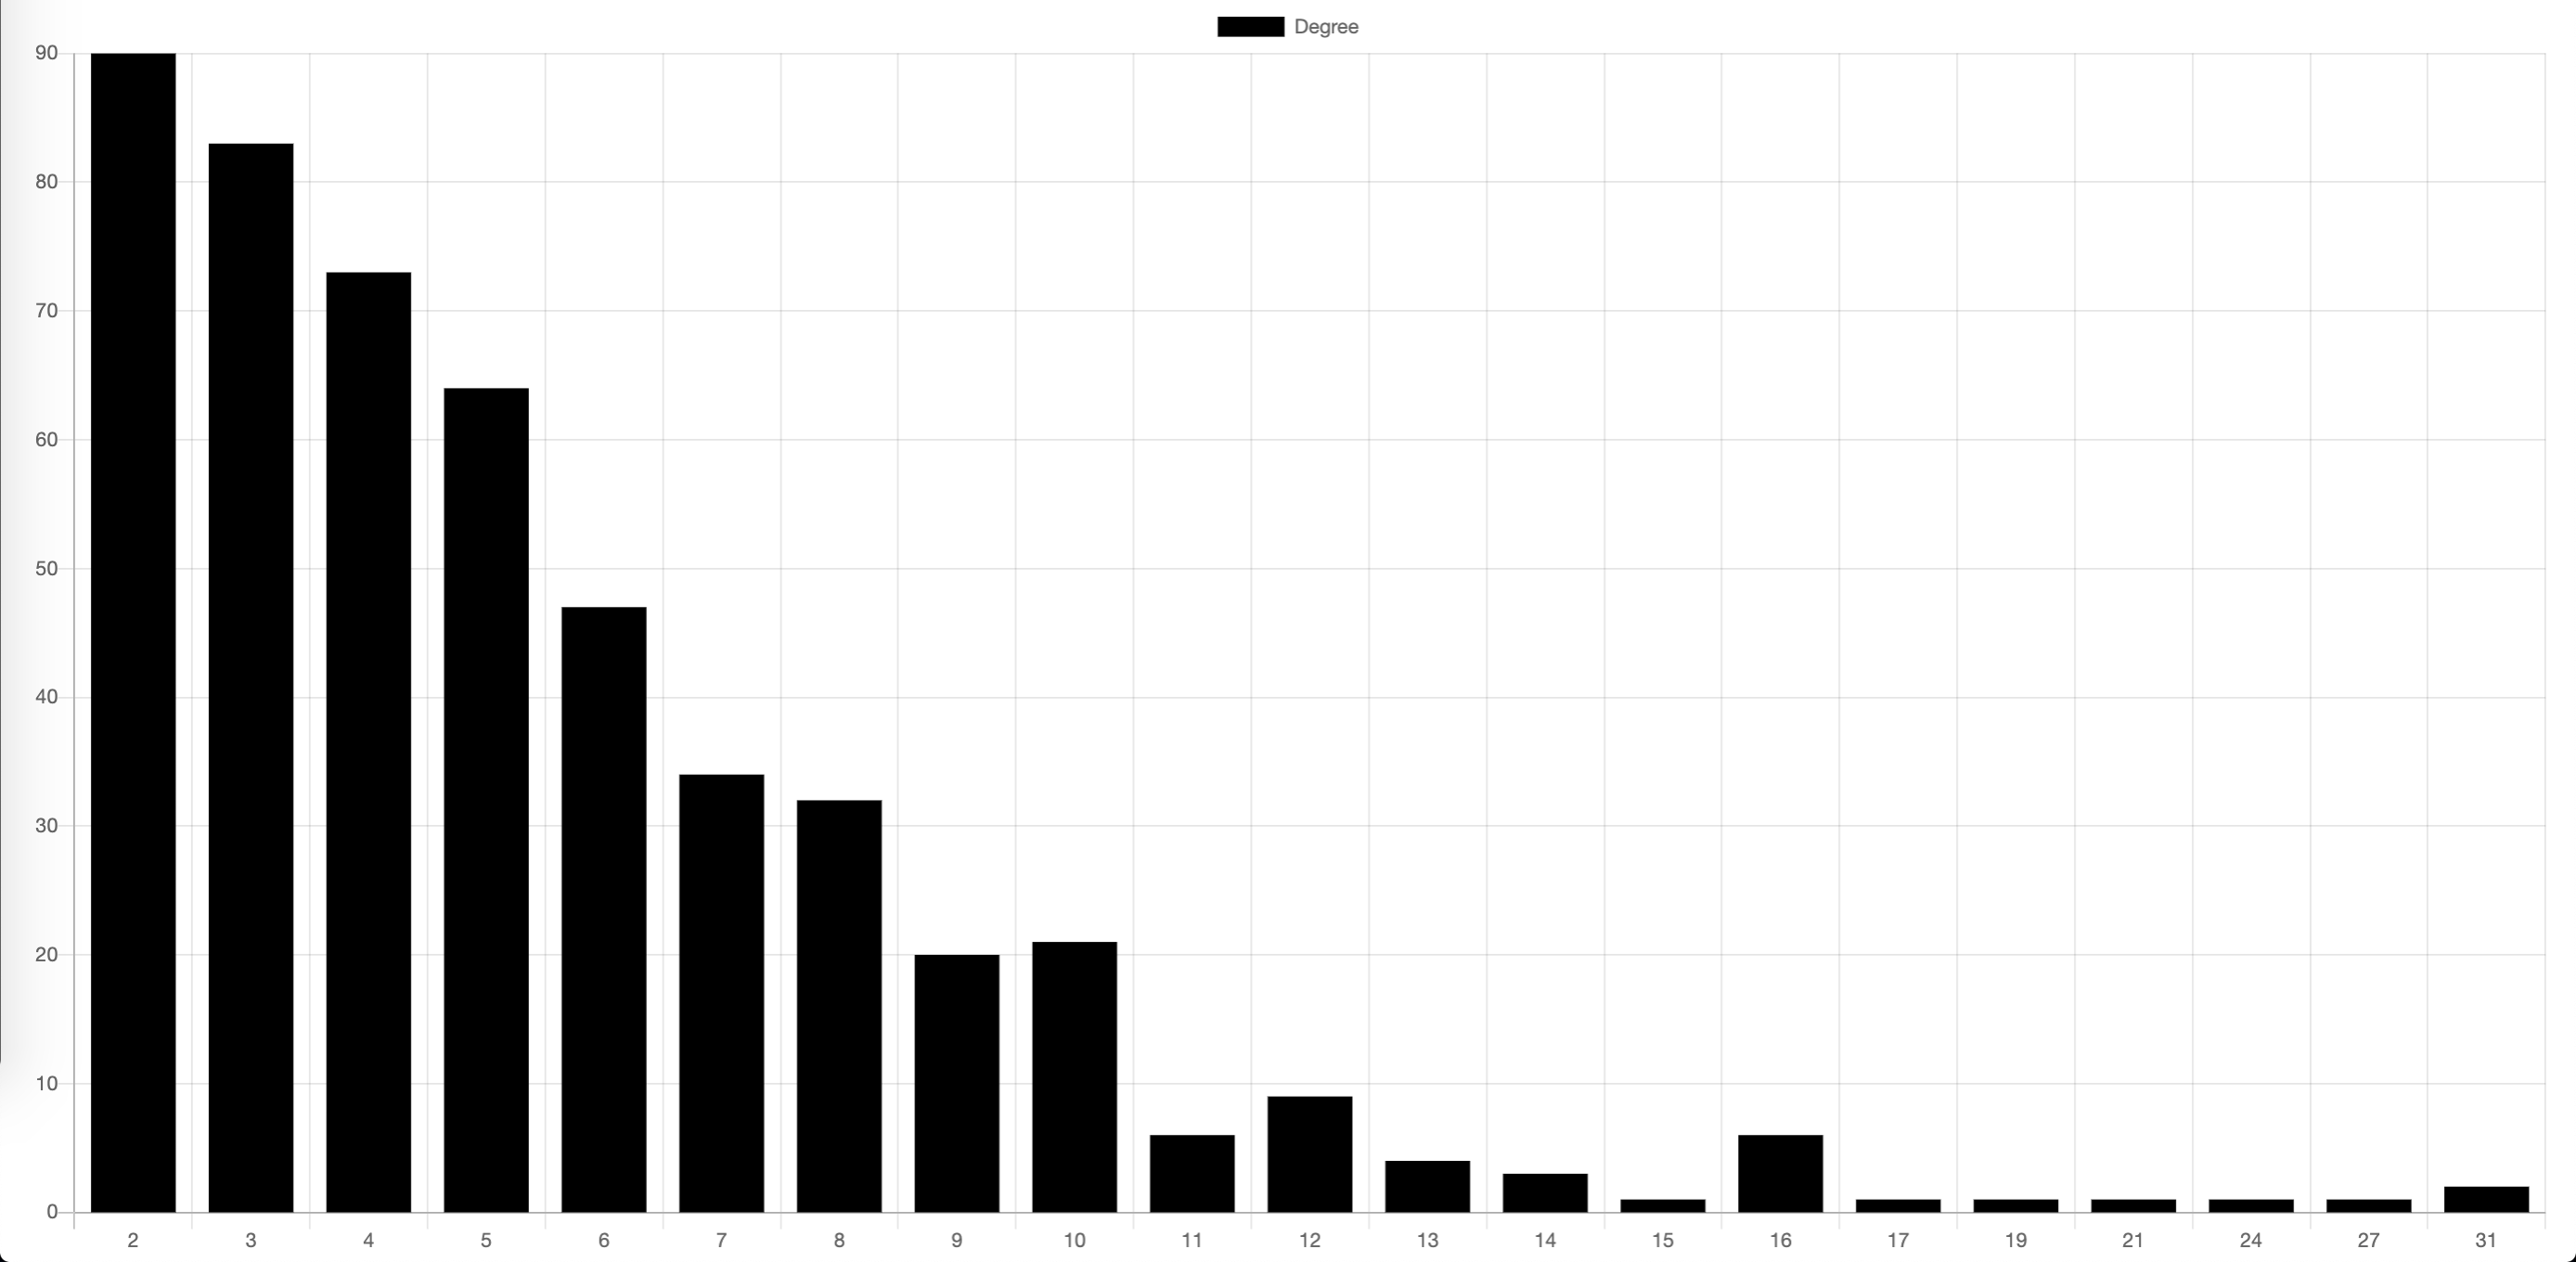
\includegraphics[width=\textwidth]{img/webOfTrust500Hist.png}
    \centering
    \caption{Degree Histogram generated by Web Of Trust algorithm for $\xi=0.5$ and $n = 500$}
    \label{fig:trustgraph500histogram}
\end{figure} 

\section{Different types of trust graph generators}

\paragraph{Probabilistic duplication}
Another trust graph generator proposed in \cite{konorski2019mitigating} base on probability duplication and can be visualized as a natural process of acquiring new colleagues at our friends' party. When we get to the party, we meet new people who with some probability become our colleagues. This algorithm works as follows: we take an initial $n_0$ nodes and $m_0$ edges and connect them randomly––creating a kernel. Then we add a new node and connect it to one random node in the current graph (your friend who invited you to his party), then with $\phi$ probability you connect to each of his friends (you acquire new friends with some of his friends), you repeat this process $n = N \textbackslash N_0$ times. 
The most important advantage of this generator is the fact that it produces scale-free graphs. Figure \ref{fig:propdup500graph} shows the graph generated by the method and Figure \ref{fig:propdup500histogram}, histogram of edge degrees.

\begin{figure}[h!]
    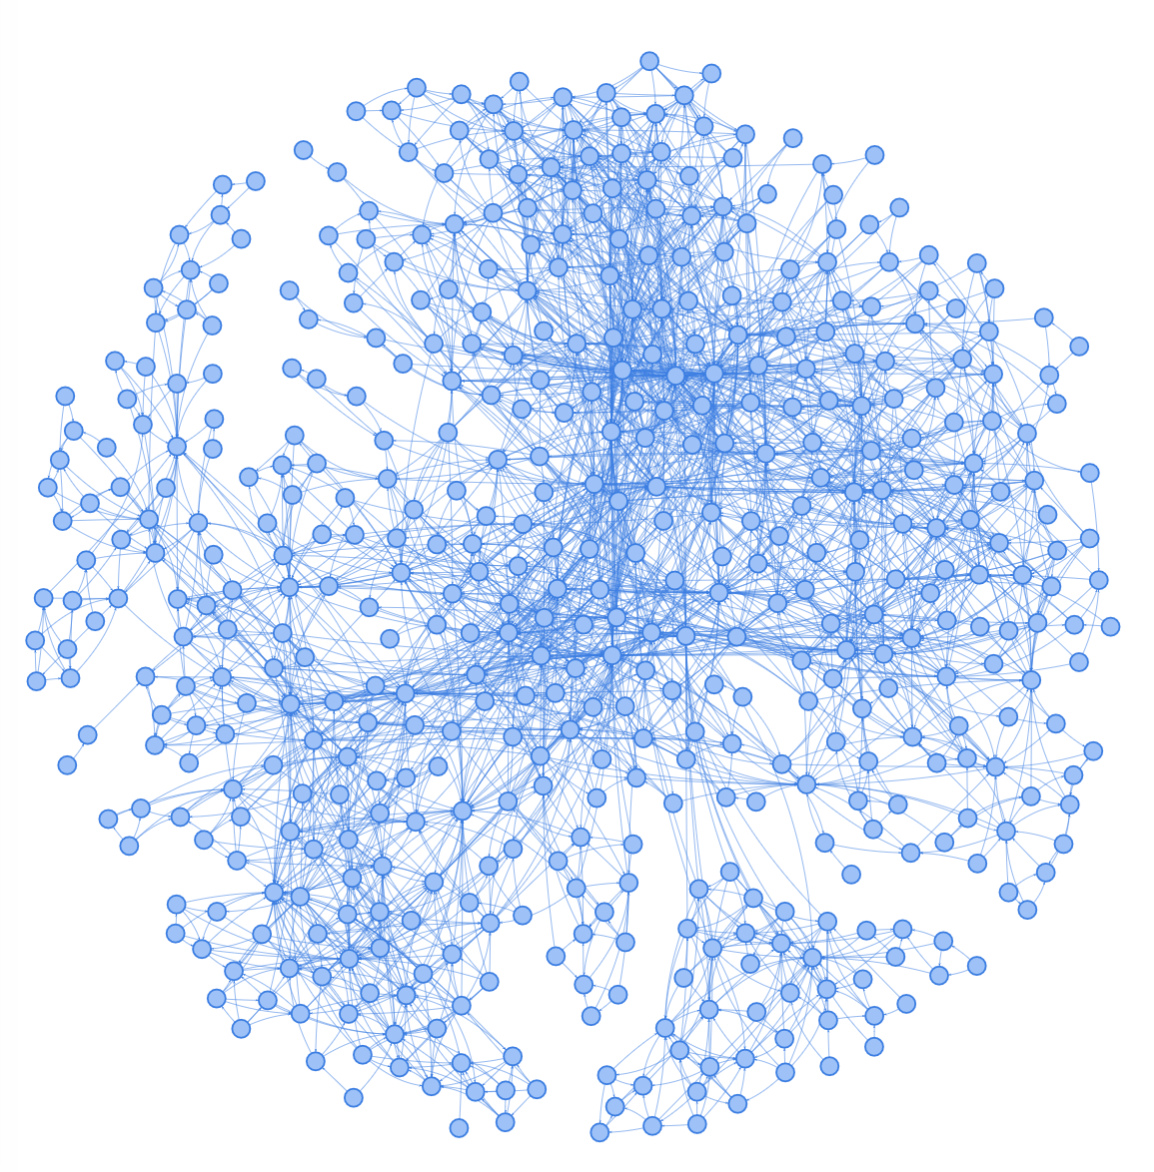
\includegraphics[width=\textwidth]{img/propDup500Graph.png}
    \centering
    \caption{Trust Graph generated by Probabilistic Duplication algorithm for $\xi=0.5$ and $n = 500$}
    \label{fig:propdup500graph}
\end{figure}

\begin{figure}[h!]
    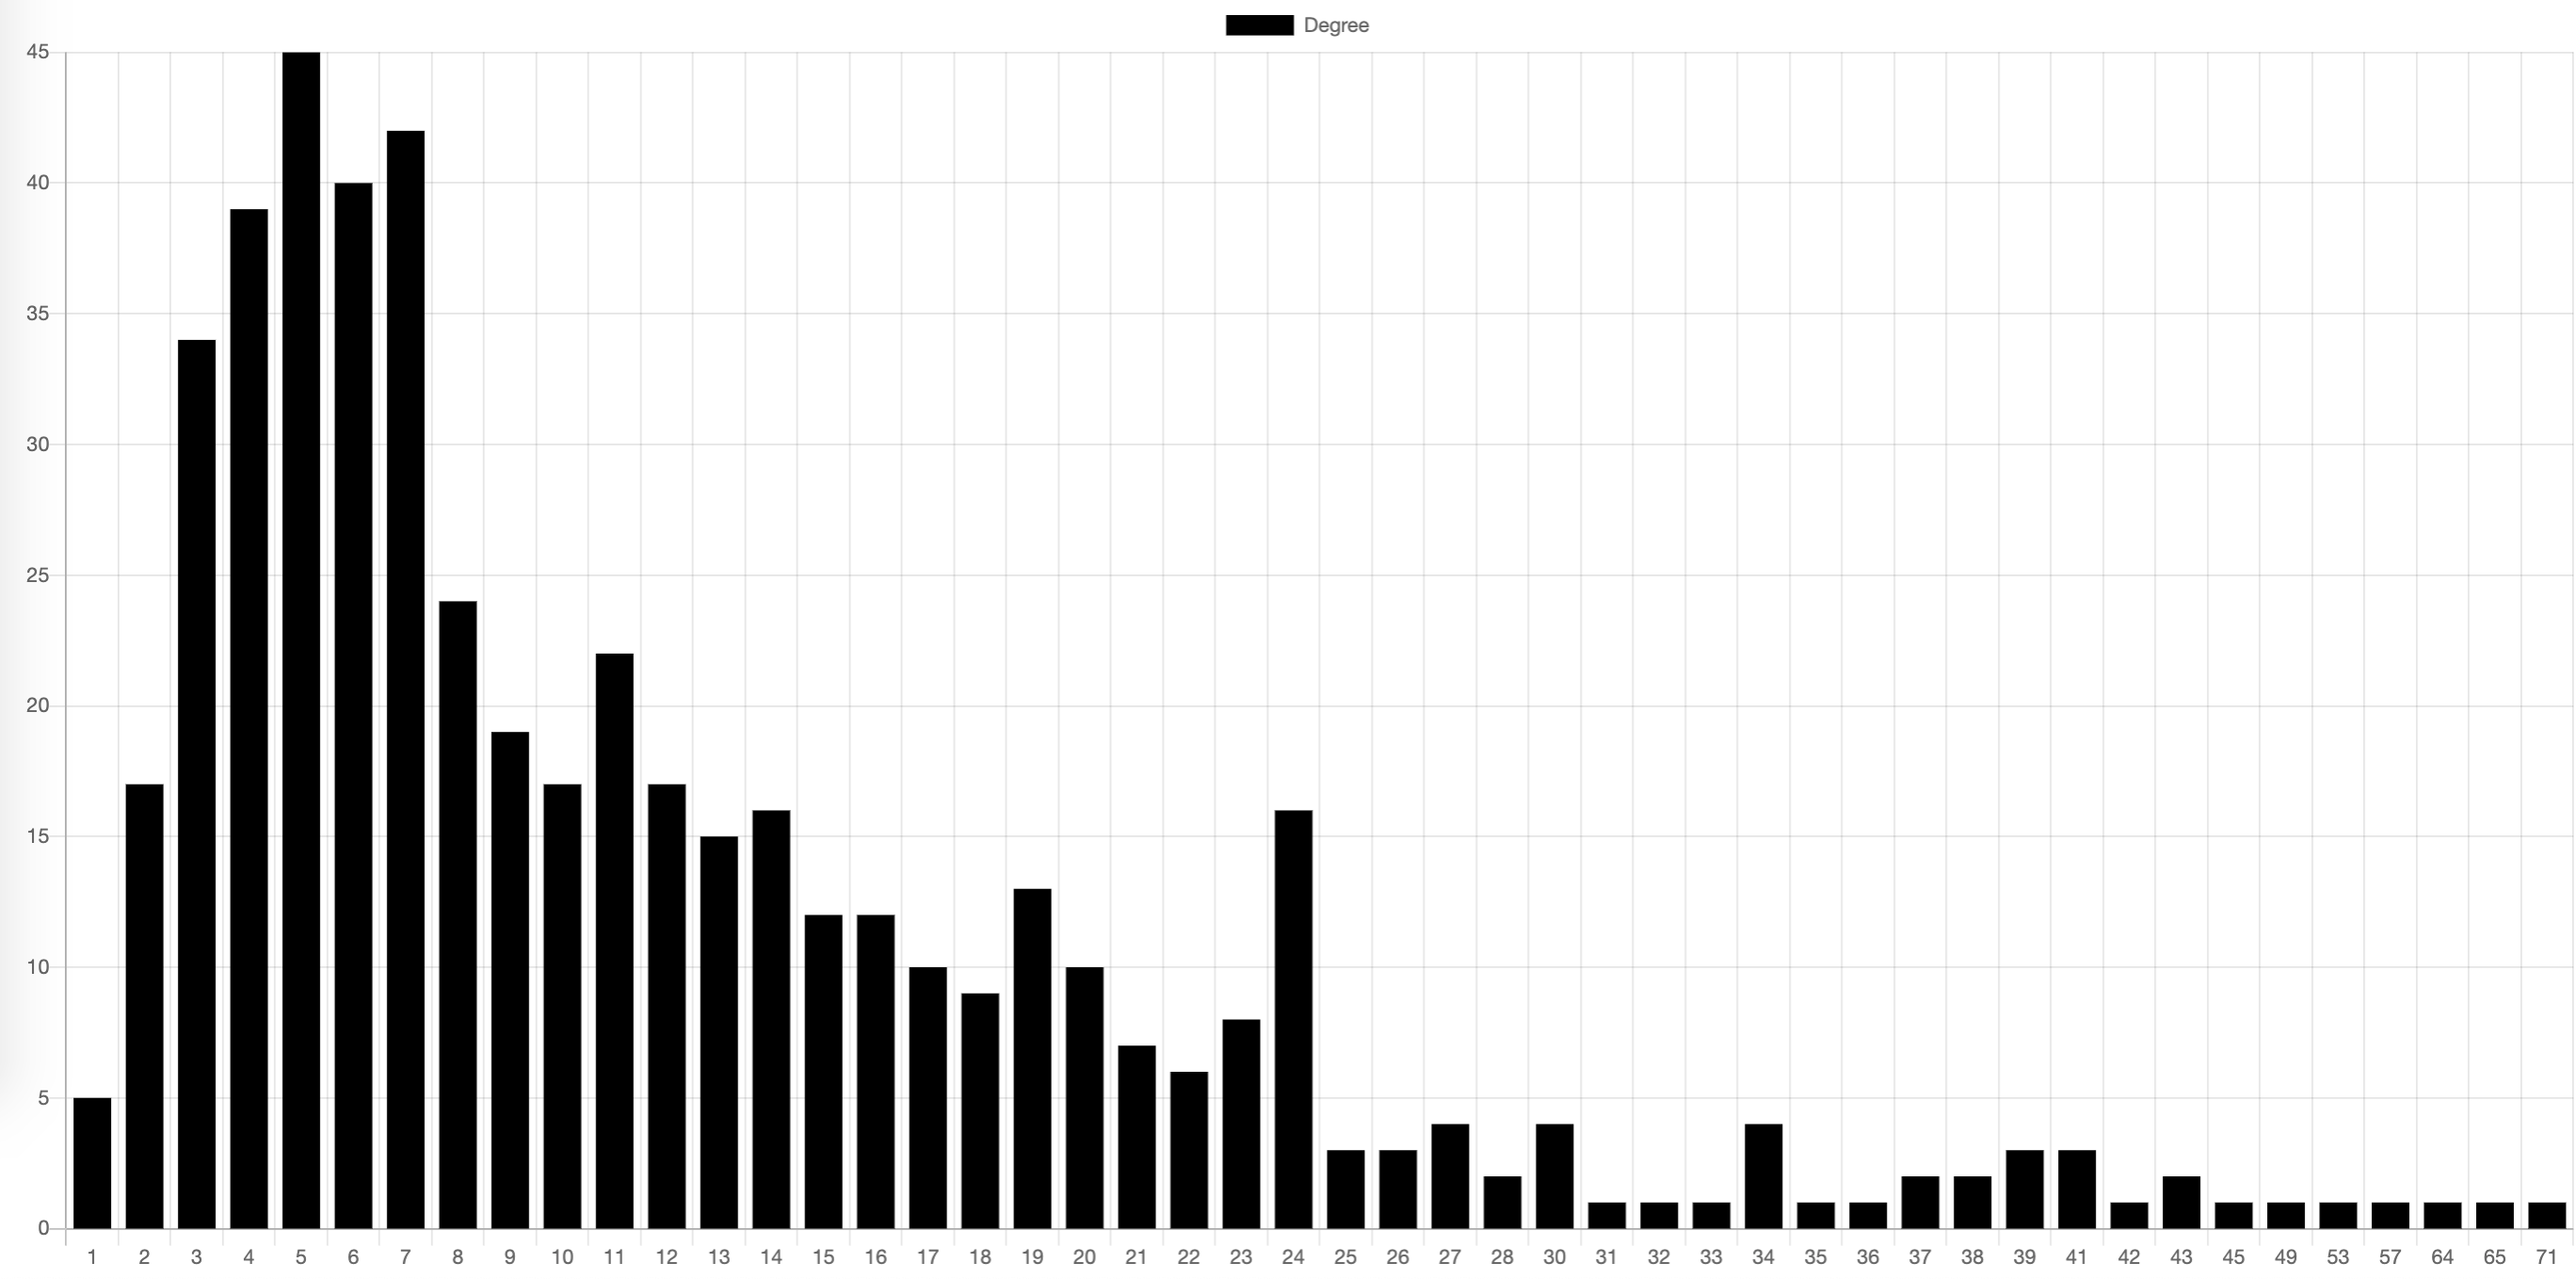
\includegraphics[width=\textwidth]{img/propDup500Hist.png}
    \centering
    \caption{Degree Histogram generated by Probabilistic Duplication algorithm for $\xi=0.5$ and $n = 500$}
    \label{fig:propdup500histogram}
\end{figure} 

\paragraph{Random generator}
Random graph generation is the simplest one. We take $n$ nodes, $m$ edges. Each edge is connected to two random nodes $n_1$, $n_2$ where $n_1 ≠ n_2$. Although random trust graphs are far from real trust graph used in reality, we will use it for comparison. Figure \ref{fig:random500graph} shows the graph generated by the method and Figure \ref{fig:random500histogram}, histogram of edge degrees.

\begin{figure}[h!]
    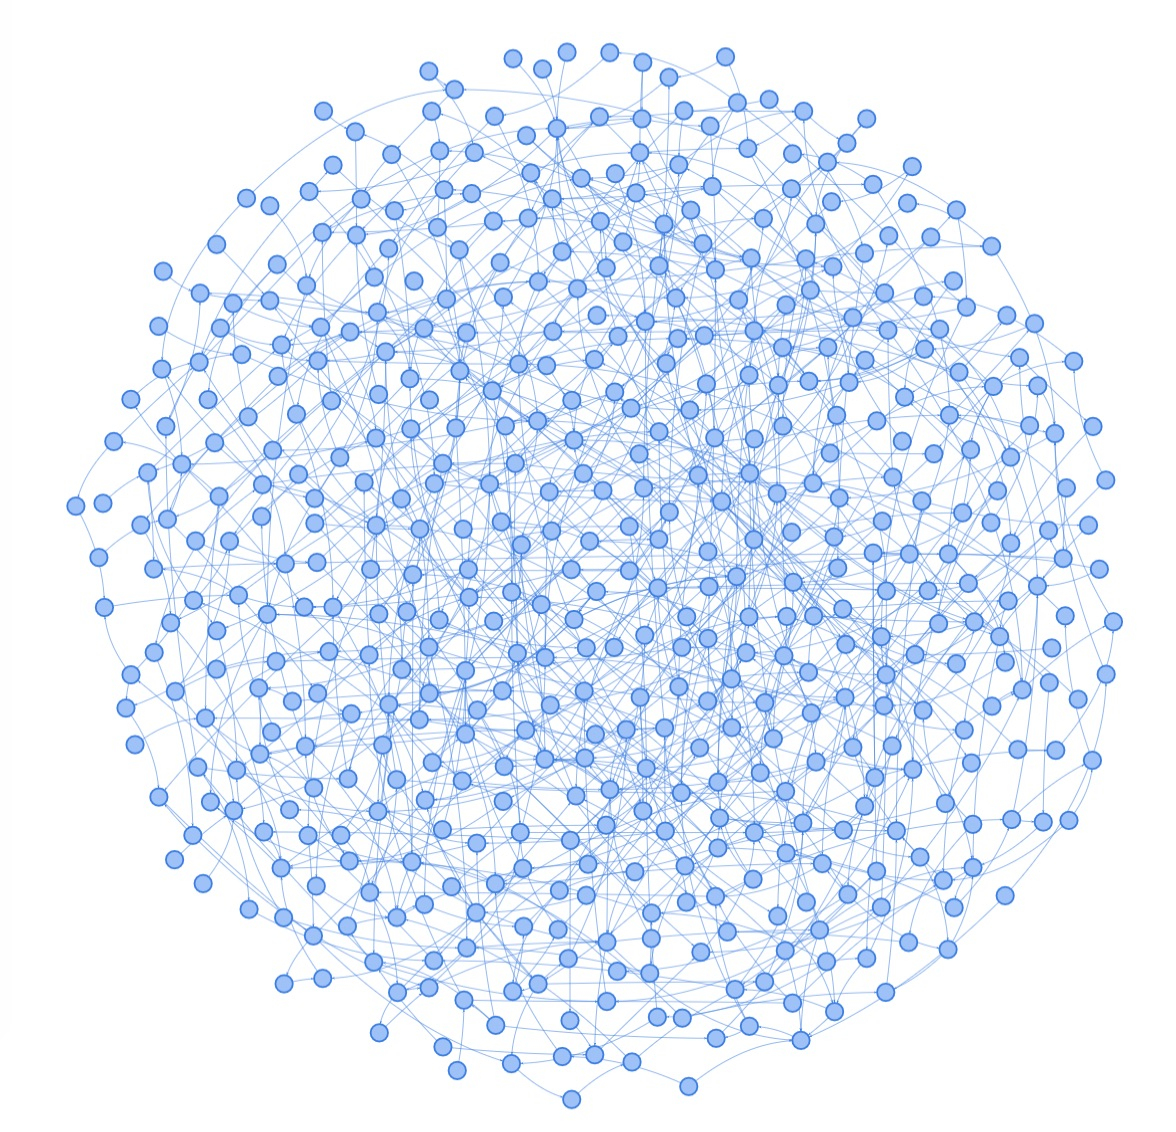
\includegraphics[width=\textwidth]{img/random500Graph.jpg}
    \centering
    \caption{Random graph generated by Random generator}
    \label{fig:random500graph}
\end{figure}

\begin{figure}[h!]
    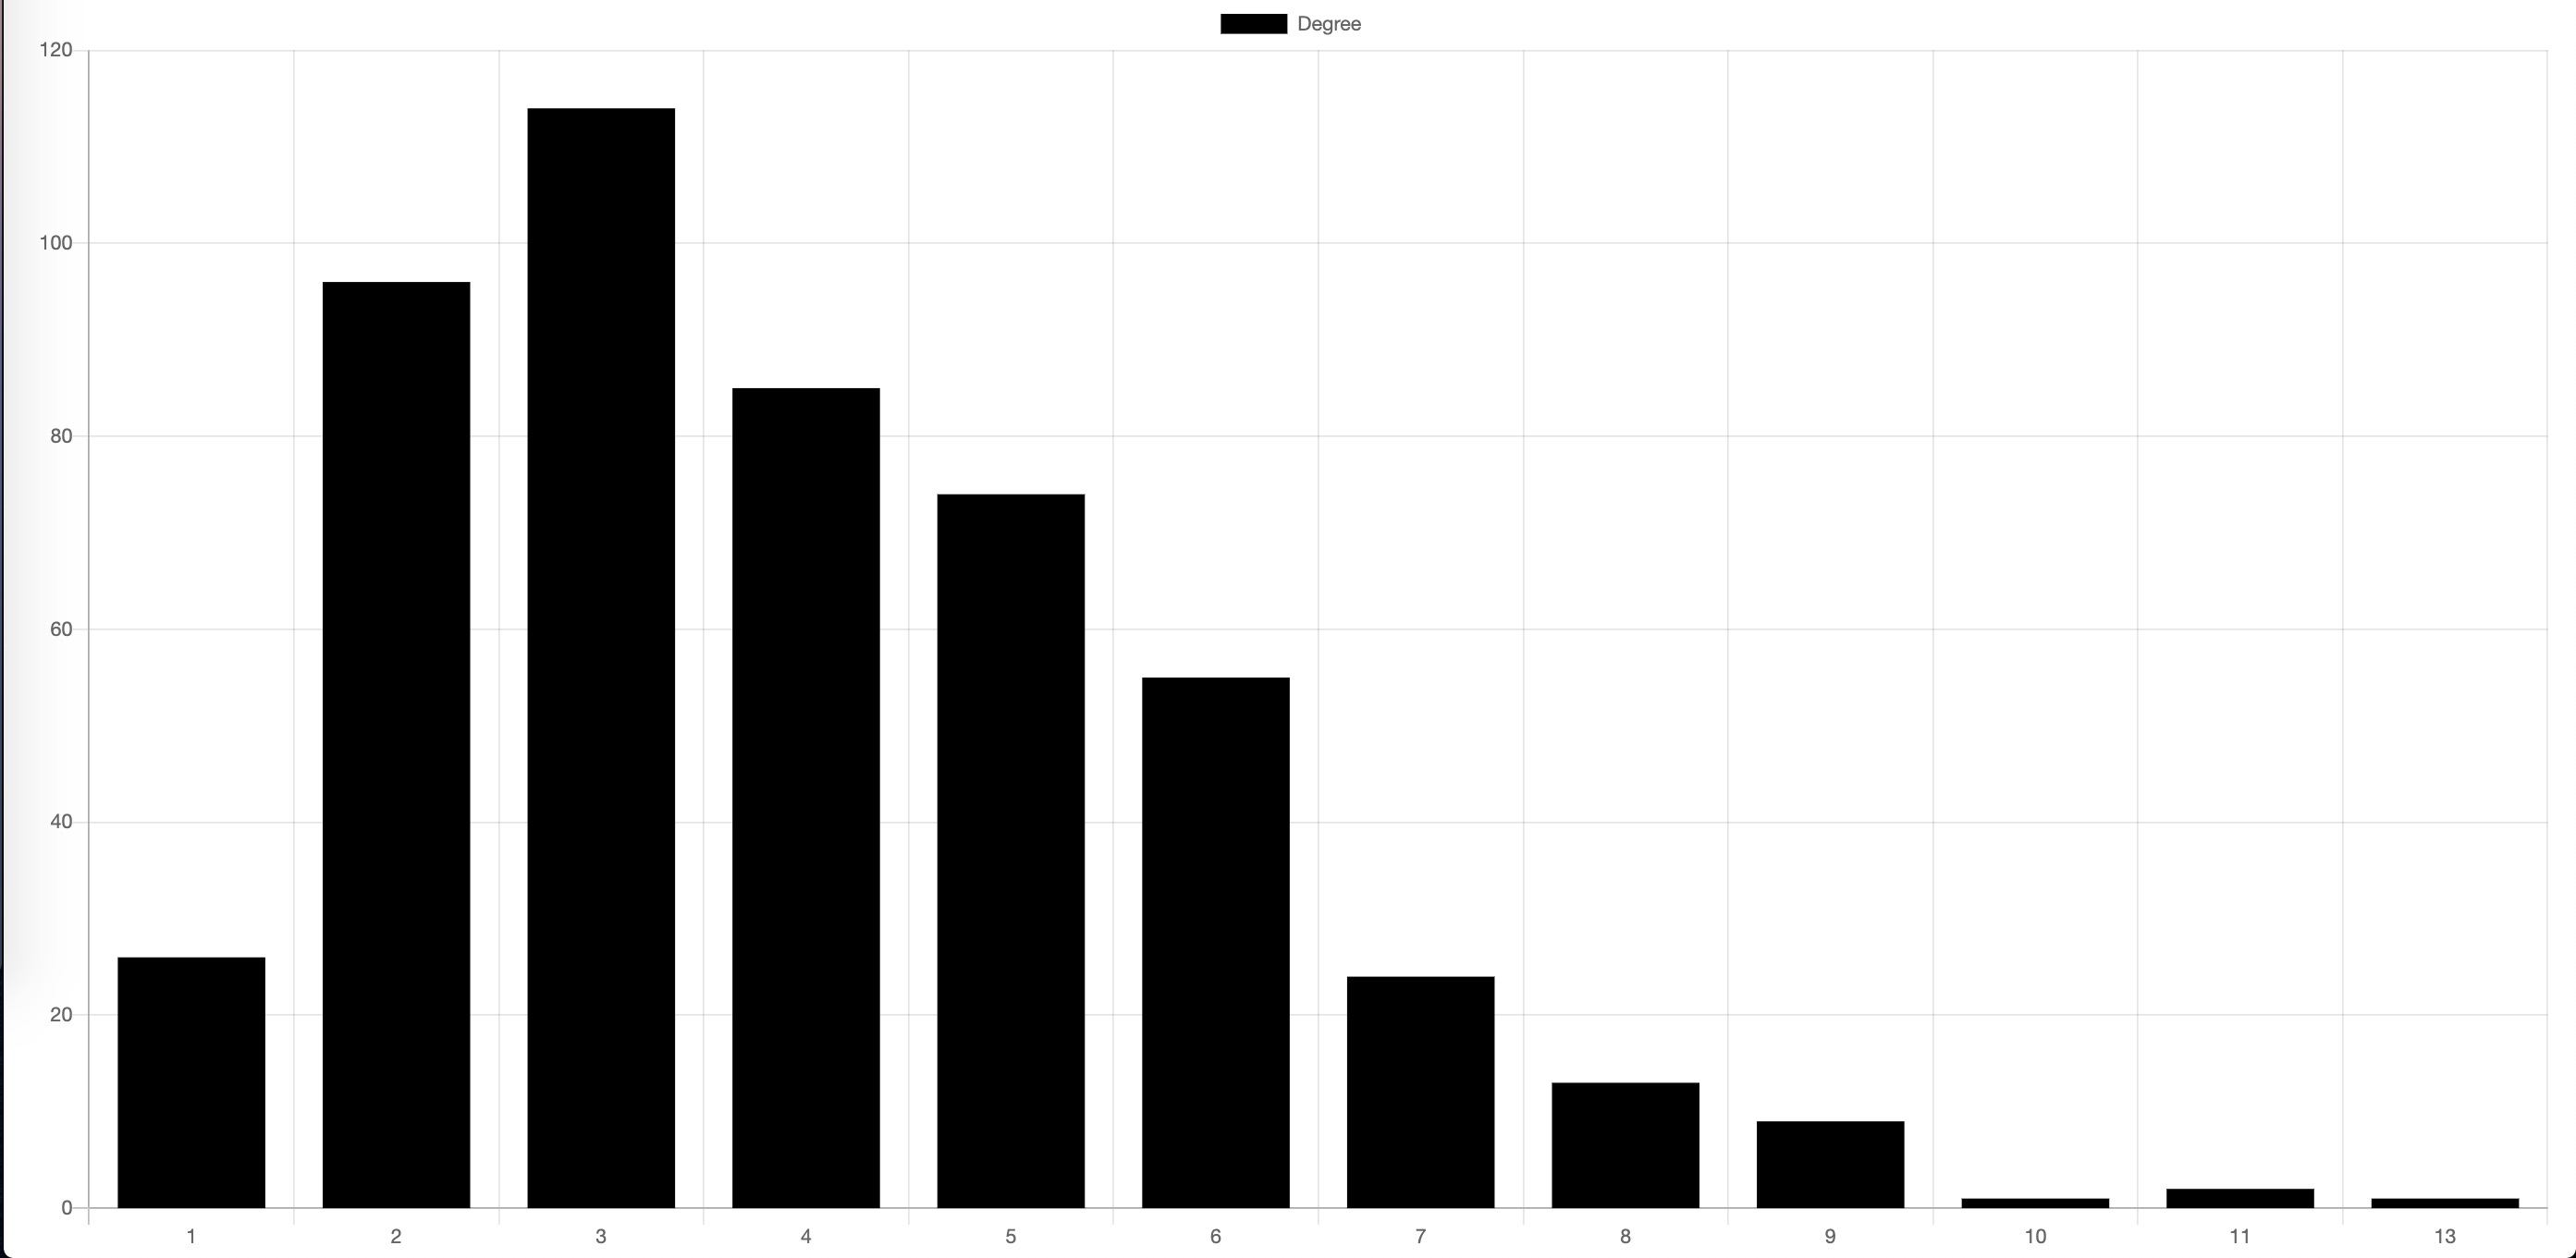
\includegraphics[width=\textwidth]{img/random500Histogram.jpg}
    \centering
    \caption{Degree Histogram generated by Random generator}
    \label{fig:random500histogram}
\end{figure} 

\chapter{Stolen Credentials Problem}
ICN authentication model is based on credentials. A unit with access to credentials can publish authenticated data, and the rest of the network has no way to verify the content authentication other than checking signature validity (created with credentials). Credentials can be loosely categorized into: cold/offline and hot/online. Cold/offline credentials, e.g., private keys, have very long (days or months) or indefinite expiration time; they are typically stored on hard drives and rarely leave the device. Hot/online credentials, e.g., access tokens, are created for a limited period (minutes or hours) and are often transmitted over a communication network. 
Stolen credentials is a serious problem that multi-factor authentication methods try to mitigate, but in this thesis we assume that even such methods cannot solve.
In conjunction with ICN caching, the problem can lead to destructive consequences, because ICN protocols do not provide data revoking/removal functions. A malicious publisher that gains access to stolen credentials can publish authenticated data that can stay in a node's cache for a long time. 

For cold/offline data breaches, we can find reports (DBIR - Data Breach Investigations Report 2020 \cite{2020Data0:online}) showing that 45\% of the attacks are caused by hacking, 22\% by misconfiguration, 22\% by phishing.  17\% caused by malicious software, 4\% by misuse by authorized users, and 4\% by physical interaction.

Most of the attacks (70\%) are performed by external entities motivated financially (86\%). Also, most attacks are targeted at big corporations (72\%). In most of them (58\%), the data breach includes users' personal information.  

From the historical data in Fig. \ref{fig:data-breach-historical} it follows that
\begin{figure}[h!]
    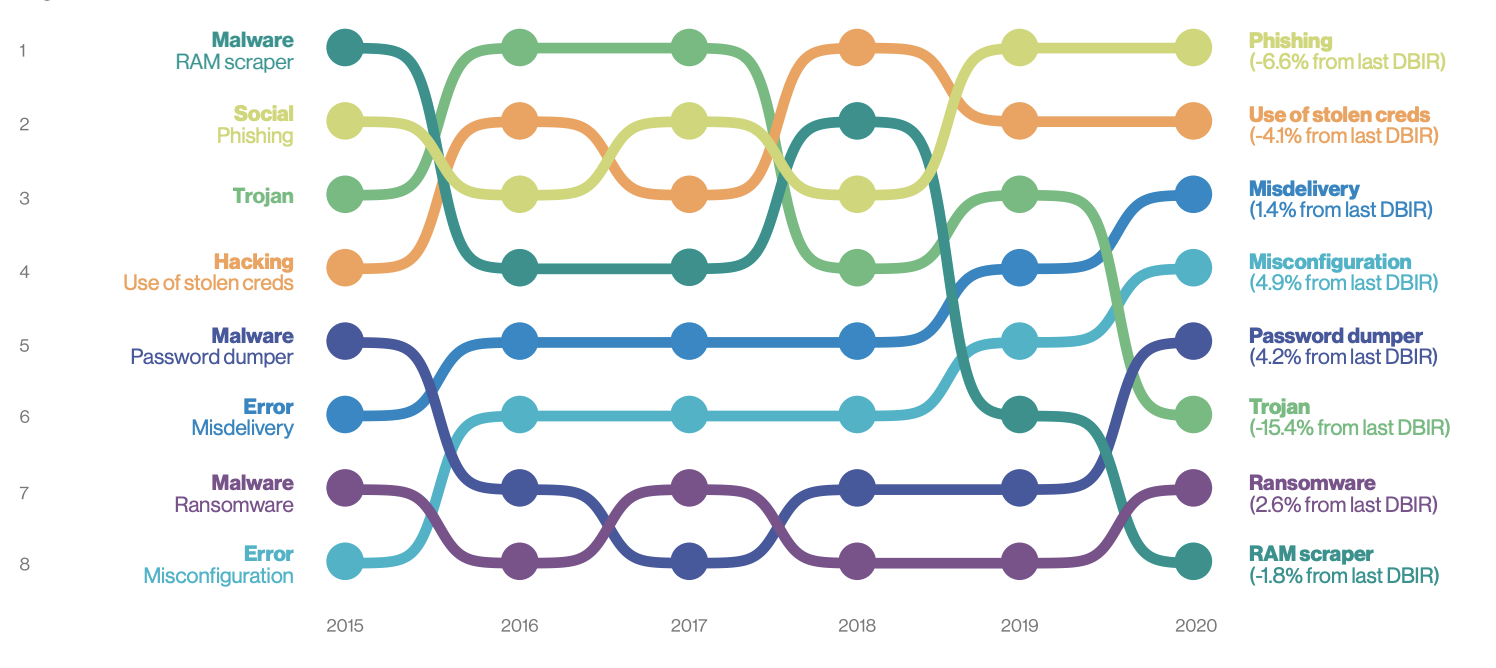
\includegraphics[width=1\textwidth]{img/data-breach-historical.png}
    \centering
    \caption{Change of breaches over time. Source: Data Breach Investigations Report 2020 \cite{2020Data0:online}}
    \label{fig:data-breach-historical}
\end{figure} 
the most visible drop occurs for Trojan horses––from 50\% in 2016 to 5.6\% in 2020. A similar drop occurs for RAM Scrapers, which search the operating system memory for potential confidential data. 
On the contrary, the highest rise can be noted for misconfiguration and accidental data leakage. Yet the highest popularity is still observed for phishing attacks and usage of stolen credentials. 
In Fig. \ref{fig:credentials-steal-discovery}, one sees that for 60\% of the incidents, \textit{the breach was discovered in less than one day}, and this trend is increasing––more incidents are discovered in less than one day. 25\% of incidents were discovered in one or more months. However, it must be noted that some breaches might not have been discovered yet, so the value may be underestimated. In this same report we can find that the number of discoveries has increased due to Managed Security Service Providers (MSSP), which are obligated to publish such breach incidents.

\begin{figure}[h!]
    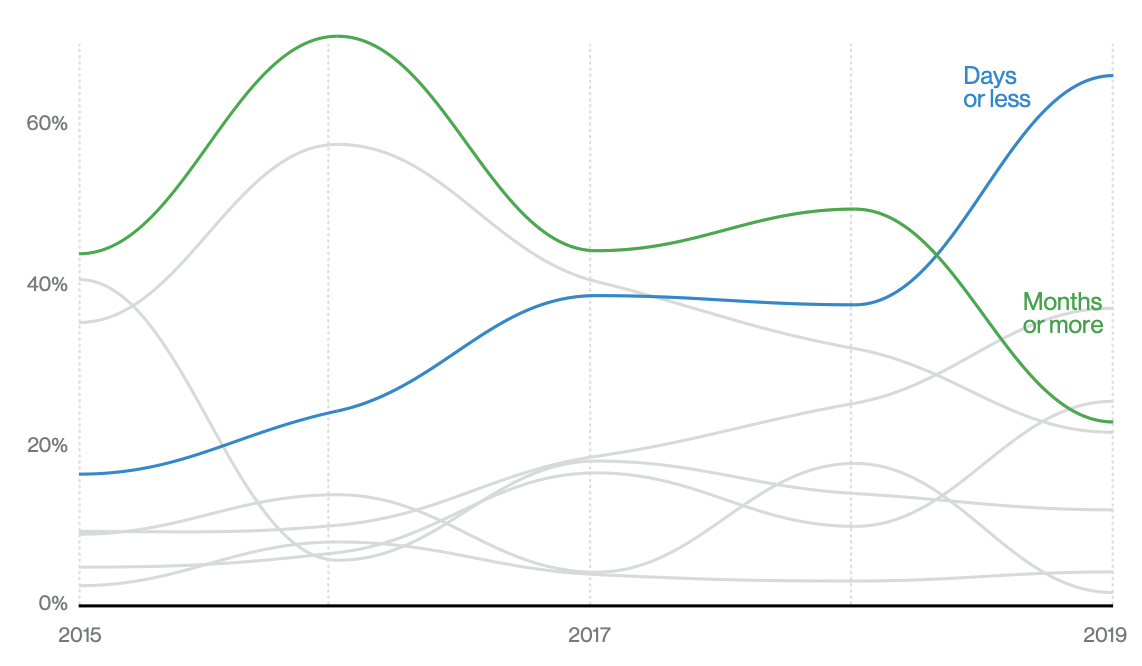
\includegraphics[width=\textwidth]{img/credentials-steal-discovery.png}
    \centering
    \caption{Discovery over time in data breaches. Source: Data Breach Investigations Report 2020 \cite{2020Data0:online}}
    \label{fig:credentials-steal-discovery}
\end{figure} 

Credentials such as access tokens (e.g., JWT tokens) used in communication between two parties have some lifetime duration, after which they expire. In the IETF RFC 6819 document \cite{RFC6819O36:online}, we can find that the suggested lifetime for such credentials ranges from minutes to hours depending on the risk associated with token leakage.
\chapter{Graph Infection}
\label{graph-infection}
The Graph Infection (GI) algorithm proposed in \cite{konorski2019mitigating} is similar to the SEIRS model, but some changes were made. There are two  healthy states--Susceptible and Quarantine, and two Infected states--Acute and Recoverable. The state transition machine is presented in Fig. \ref{fig:finite-state-machine-jekon}.
\begin{figure}[h!]
    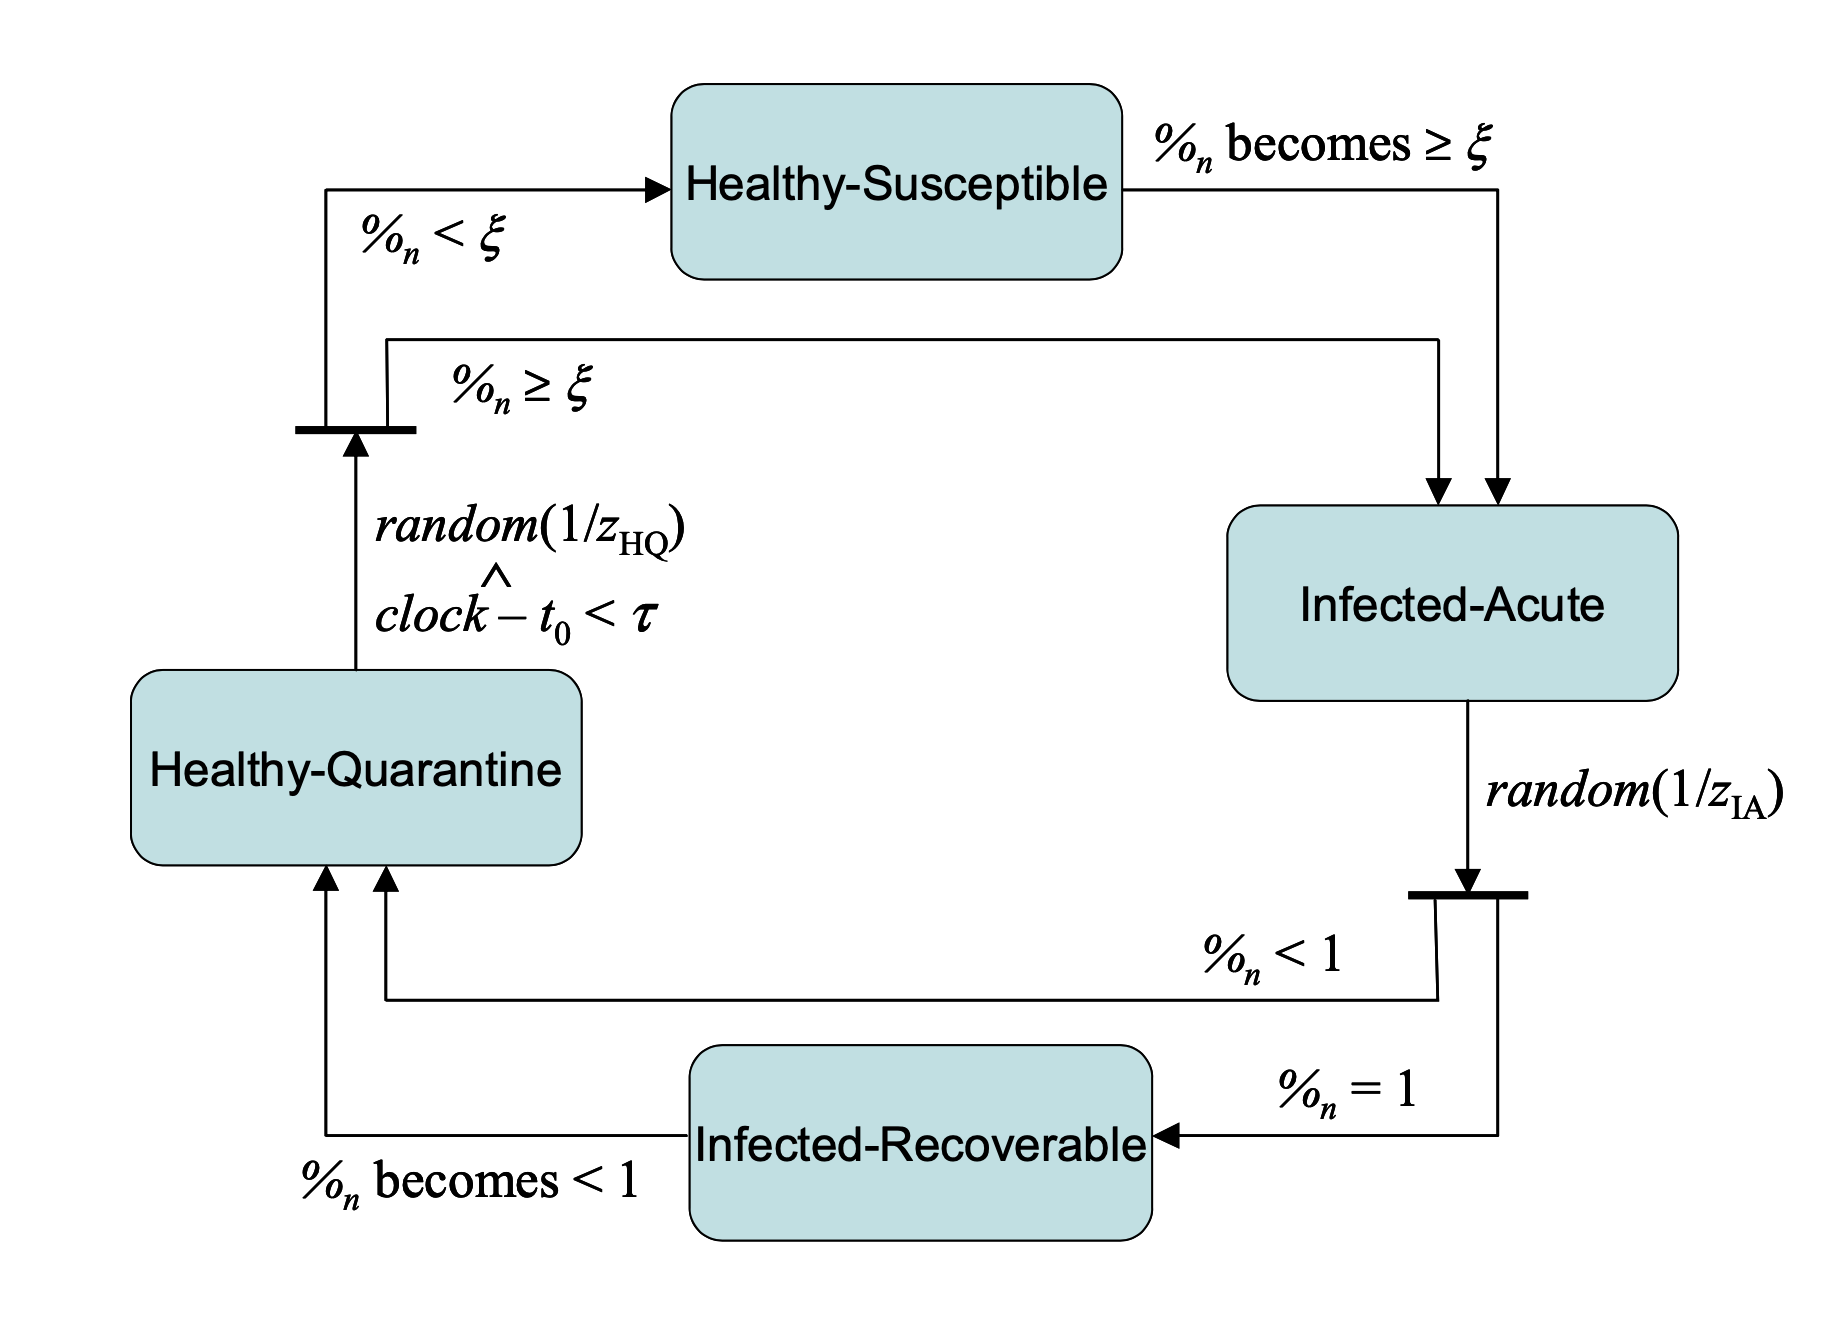
\includegraphics[width=11cm]{img/finite-state-at-node.png}
    \centering
    \caption{Finite state machine at a node. Source: Mitigating Time-Constrained Stolen-Credentials Content Poisoning in an NDN Setting \cite{konorski2019mitigating}}
    \label{fig:finite-state-machine-jekon}
\end{figure} 

The four states can be described as follows:
\begin{itemize}
\item Susceptible nodes are healthy––they do not propagate infection, but can get infected, whereupon change state to Acute.
\item Acute nodes are infected––they inflict infection propagation and switch state to Recoverable or Quarantine depending on how many of their neighbors are infected.
\item Recoverable nodes are infected but can switch to Quarantine if some of their neighbors become healthy.
\item Quarantine nodes are healthy and can switch state to Susceptible or Acute, depending on how many of their neighbors are infected.
\end{itemize}
Nodes can get infected by either:
\begin{enumerate}
    \item external infection -- a content publisher can always infect his/her home node, and then successive nodes at fixed time intervals.
    \item internal infection -- when the fraction of infected neighbors surpasses the $\xi$ threshold. 
\end{enumerate}

Initially, all nodes are healthy (distrust new content). When a publisher wants to authenticate new content, he/she starts the external infection process by infecting his/her assigned home node. The home node imposes a fixed delay, after which it issues a new certificate allowing the publisher to infect the next node selected at random. The publisher infects the next node by presenting the certificate signed by the previous node. This process is repeated until an epidemic occurs or the intruder loses access to the stolen credentials. To give this process some momentum, we allow the infected nodes to infect others in a process of internal infections. In this way, the publisher does not need to coordinate the whole process until the network reaches epidemic, but just starts a "chain reaction", and if he/she does so with sufficient power, an epidemic will occur.

Internal infections work as follows: a node $n$ in the Susceptible state switches to the Acute state by being infected by a sufficient proportion of its neighbors, specifically if the fraction of its infected neighbors $\%_n = \frac{|I_n|}{|N_n|}$ reaches the threshold $\xi$, where $I_n$ is the set of infected $n$'s neighbors and $N_n$ is the set of all $n$'s neighbors. For simplicity let us measure time in units called \textit{cycles}, a cycle being long enough for a node to infect a neighbor node. To give the process some momentum, the Acute and Quarantine states are introduced. A node has to spend some random time before leaving either state, denoted $random(\frac{1}{Z_{IA}})$ and $random(\frac{1}{Z_{HQ}})$, respectively, where $Z_{IA}$ is the mean number of cycles in the Acute state, and $Z_{HQ}$ is the mean number of cycles in the Quarantine state. Depending on $\%_n$, a node leaving the Acute state switches either to Recoverable––if $\%_n = 1$, or directly to Quarantine––if $\%_n < 1$. In the Recoverable state, the node is still infected, but as soon as one of its neighbors recovers, it switches to the Quarantine state. The Quarantine state is similar to Acute except that a node can be locked in this state forever if it gets immunized. The immunization is acquired after $\tau$ cycles from the first infection on the node, where $\tau$ is a fixed parameter working as a timeout, preventing an endemic (partial epidemic) of the network. If an endemic were to prevail for a long time, it would mean that the publisher's proof-of-time was too weak to reach an epidemic, but too strong for all the nodes to recover.

As we discussed earlier, there is no known analytical solution to such a graph model; therefore, it needs to be computer simulated.

\section{Simulator}
\label{simulator}
\begin{figure}[h!]
  \subfloat[Visual simulator]{
	\begin{minipage}[c][1\width]{
	   0.5\textwidth}
	   \centering
	   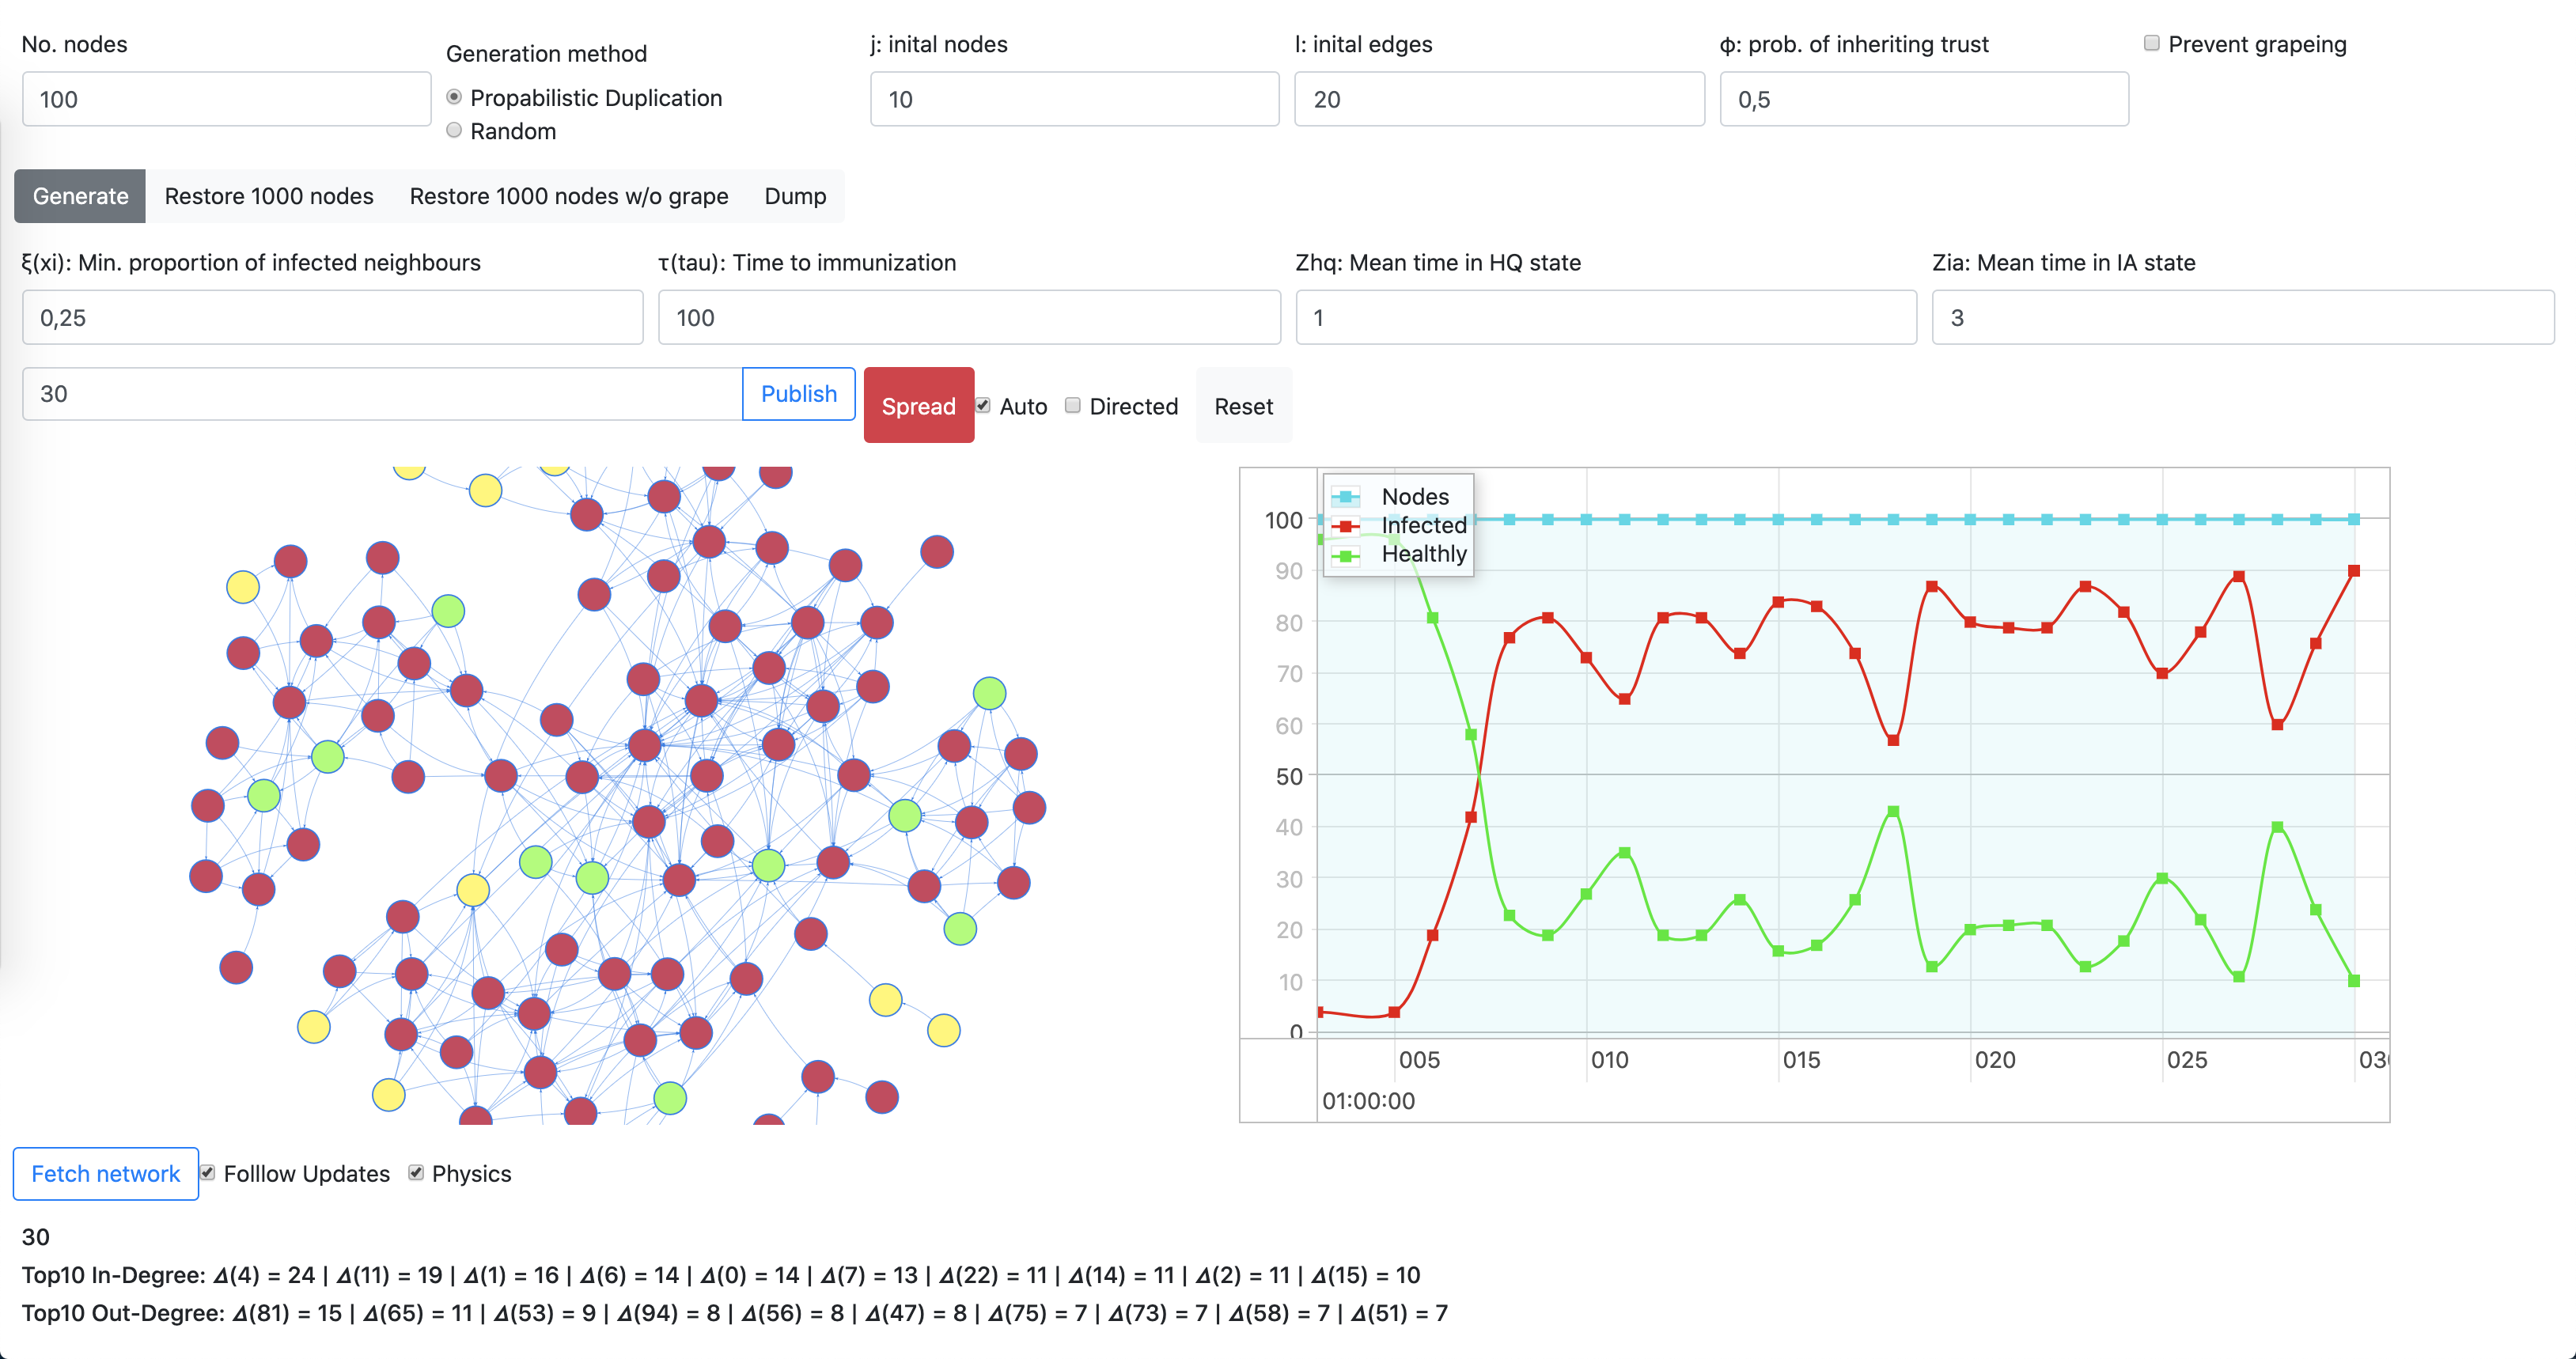
\includegraphics[width=1\textwidth]{img/simulator.png}
	\end{minipage}}
 \hfill 	
  \subfloat[Fast simulator]{
	\begin{minipage}[c][1\width]{
	   0.5\textwidth}
	   \centering
	   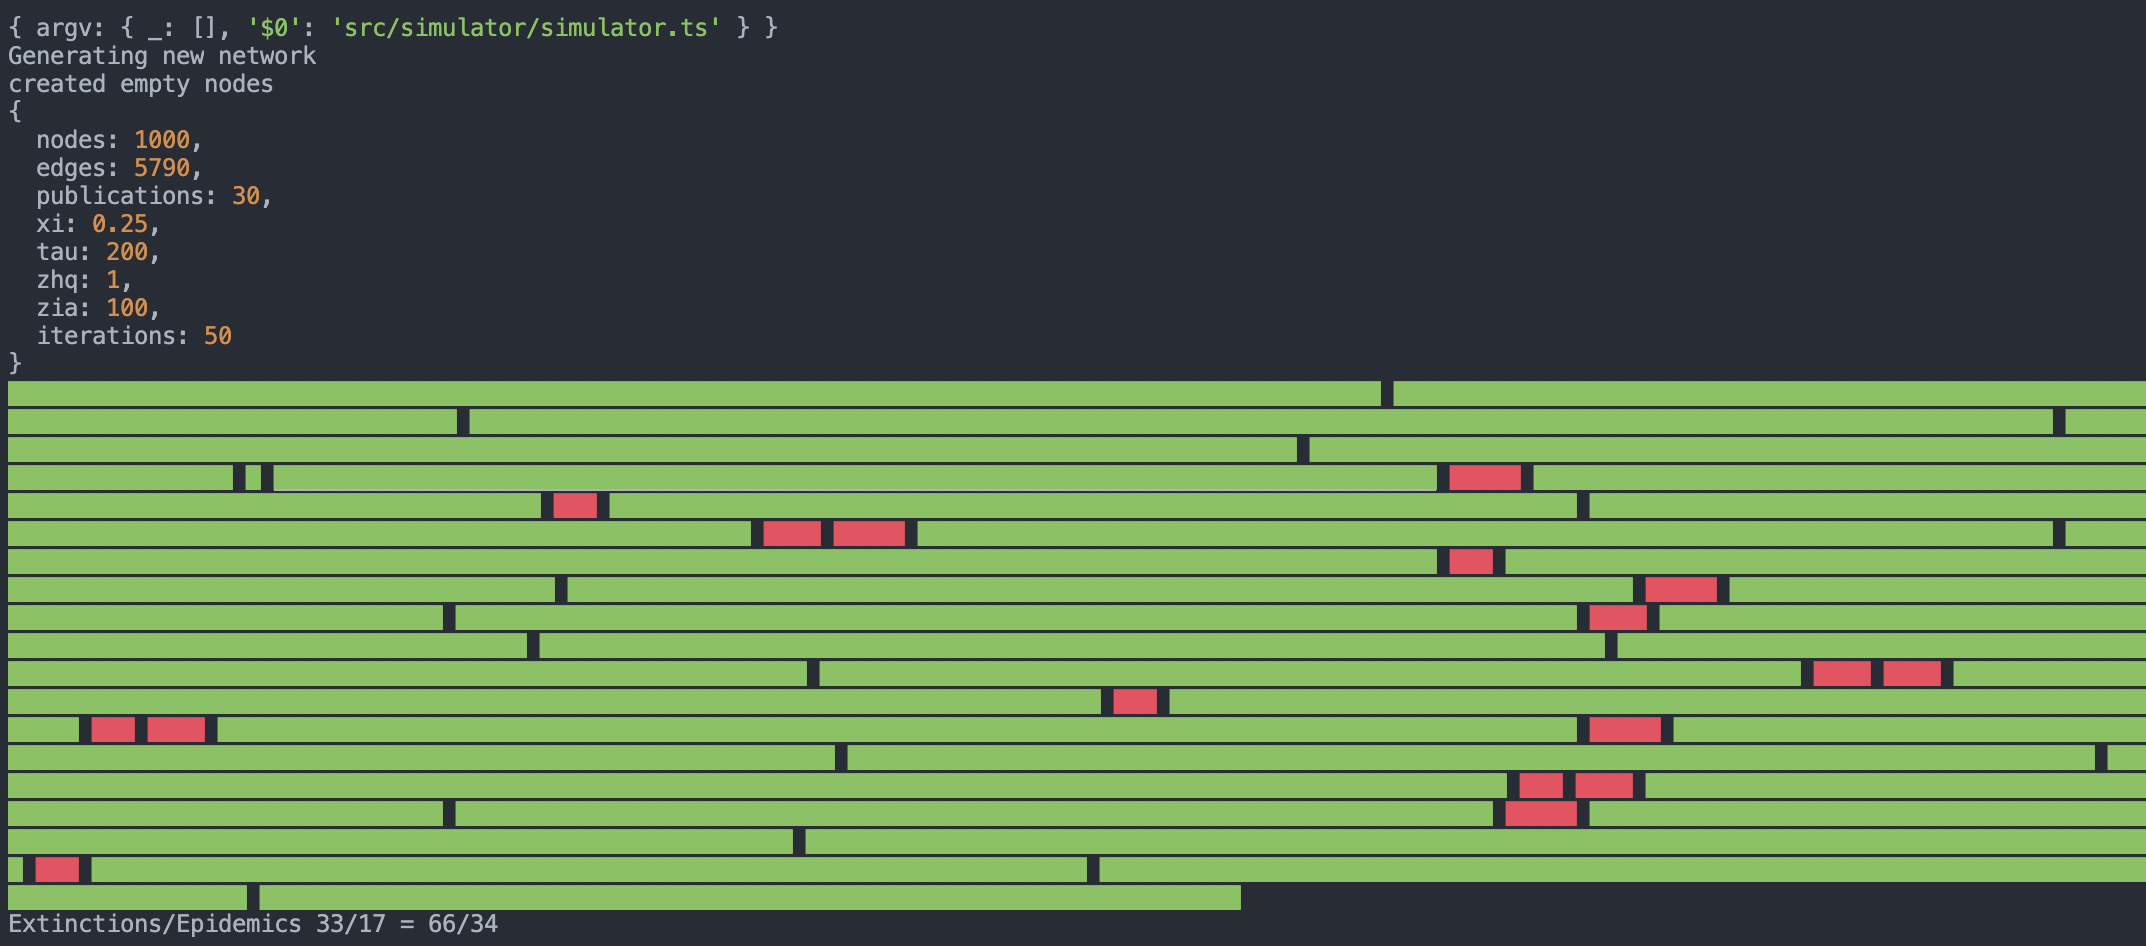
\includegraphics[width=1.1\textwidth]{img/fastsimulator.png}
	\end{minipage}}
\caption{Simulators preview}
\label{fig:simulators}
\end{figure}
We have developed two simulators, the first for visualization and the second for fast calculations. The visualization simulator helps to better understand the processes on graphs and find potential problems. The fast simulator allows to perform various calculations on different input data in a reasonable time. The source code for both simulators is available at \url{https://github.com/stasbar/ProofOfTime-Auth}. Both simulators are presented in Fig. \ref{fig:simulators}. The visual simulator is accessible at \url{masti.stasbar.com}.
Both simulators allow us to generate the trust graph using three different generators: random, web of trust, and probabilistic duplication discussed in Chapter \ref{trust-graph} with customized parameters: number of nodes, number of nodes and edges in the initial kernel, and $\phi$, used in the web of trust and probabilistic duplication to customize the density of the connections. After the graph is generated, one can save and restore it to always work on the same graph during further research. 
When the graph is loaded, we can configure the parameters $\xi$, $\tau$, $Z_{HQ}$, $Z_{IA}$ and the number of external infections (i.e., publications or proofs-of-time).
The fast simulator outputs the results of simulations; the green color indicates that the network ended up in an extinction (all nodes have recovered) and the red color indicates an epidemic; the length of the block indicates the number of cycles needed to reach one of these outcomes. The visual simulator provides a live preview of the graph and a chart of the ongoing infection process.  


\section{Observations}
\label{observations}

We run the simulator against many different configurations to find the influence of each parameter. The algorithm's probabilistic nature forces us to run the simulation multiple (in our case, 200) times for each configuration to get credible results. We run the simulation on 1000-node graphs generated using both web of trust (WoT), random(RND), and probabilistic duplication (PD) generators, but for each simulation, we use the same generated graph. First we investigate the $Z_{IA}$ parameter by assuming all remaining parameters constant: $\xi=0.25, Z_{HQ} = 1, \tau=200$ with the maximum number of external infections (publications) equal to 300.
\begin{figure}[h!]
    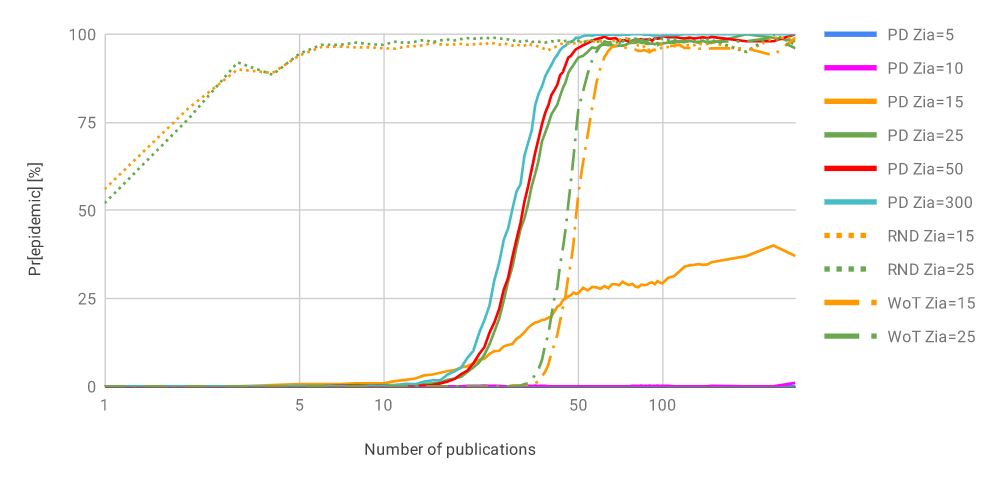
\includegraphics[width=\textwidth]{img/influence-of-zia.png}
    \centering
    \caption{Influence of $Z_{IA}$ parameter}
    \label{fig:influence-of-zia}
\end{figure} 
Figure \ref{fig:influence-of-zia} shows how $Z_{IA}$ influences the probability of reaching an epidemic, (Pr[epidemic]), against the number of external publications (proof-of-time). It does not come as a surprise that the higher $Z_{IA}$, the longer nodes stay infected, and the faster an epidemic is reached. The PD and WoT graphs produce similar shapes. The WoT graph starts to reach an epidemic a little later. 
The RND graph is completely different; even with a low $Z_{IA}$, it reaches an epidemic with just one publication. It happens because most of the nodes have only one or two edges. As a result, one infected node can infect most of its neighbors. In contrast, the PD and WoT graphs often produce nodes of a high degree that are hardly infected by their neighbors.
For all graphs with $Z_{IA}$ starting from 25, the chance of reaching an epidemic in near 100\% starts at about 50-80 external publications. E.g., if we assume the required proof-of-time amounts to 12h, the publisher needs to publish the proof-of-time each 9 to 14 minutes until an epidemic becomes certain.

\begin{figure}[h!]
    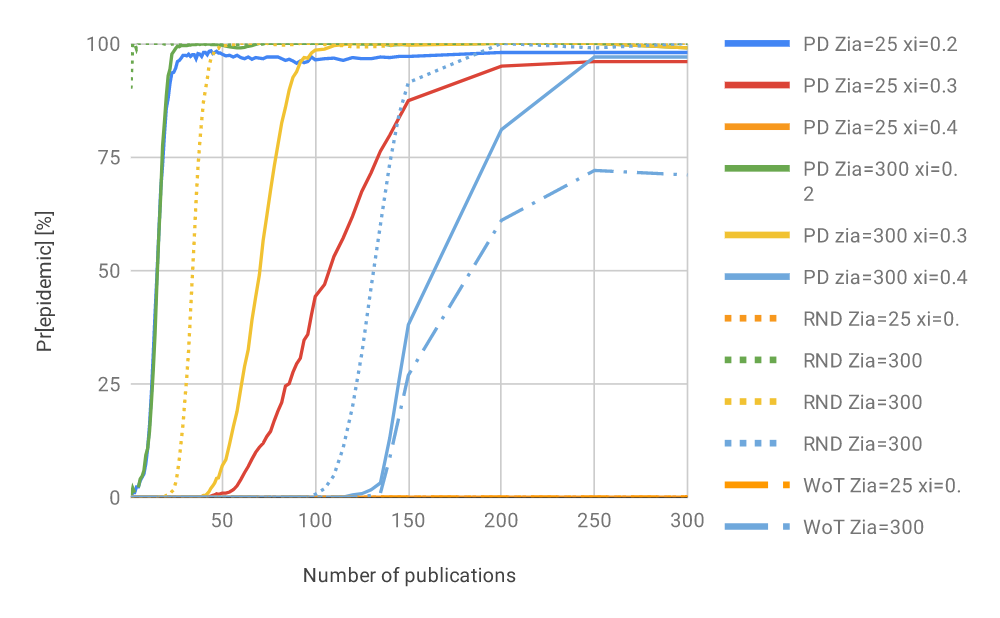
\includegraphics[width=\textwidth]{img/influence-of-xi.png}
    \centering
    \caption{Influence of $\xi$ parameter}
    \label{fig:influence-of-xi}
\end{figure} 
In a similar way, we test the $\xi$ value. Figure \ref{fig:influence-of-xi} shows the Pr[epidemics] against the proof-of-time using different $\xi$ values. We can easily see that $\xi$ is the most sensitive parameter. For values starting from $\xi=0.5$ not a single epidemic simulation occured for any graph generator.

\begin{figure}[h!]
    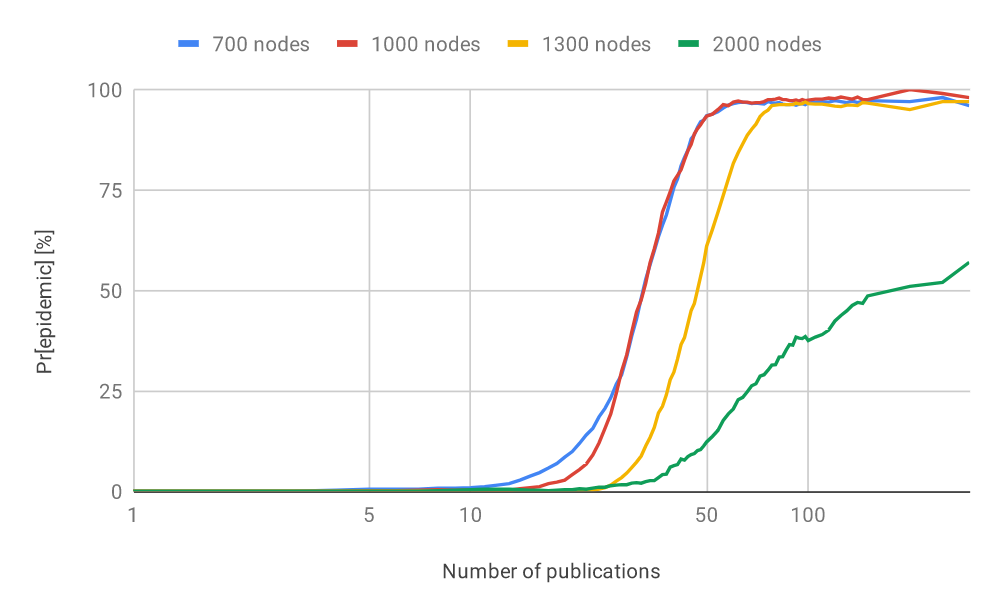
\includegraphics[width=\textwidth]{img/Influence-of-network-size.png}
    \centering
    \caption{Influence of network size}
    \label{fig:influence-network-size}
\end{figure} 
We notice that the parameters $Z_{ia}$ and $xi$ can completely change the outcome depending on the graph type. Their universal values may be hard to find if we want a solution that works on all types of trust networks. Moreover, if we want to set a fixed number of external publications needed to achieve an epidemic, those values should be dynamically changed according to the size of the network.
For example for $\xi=0.25$, $Z_{IA}=25$, $Z_{HQ}=1$, $\tau=200$ the probability of epidemic is significantly influenced by the size of the graph (see Figure \ref{fig:influence-network-size}). Therefore we believe that those parameters should be dynamically adjusted with the network structure changes.

\begin{figure}[h!]
    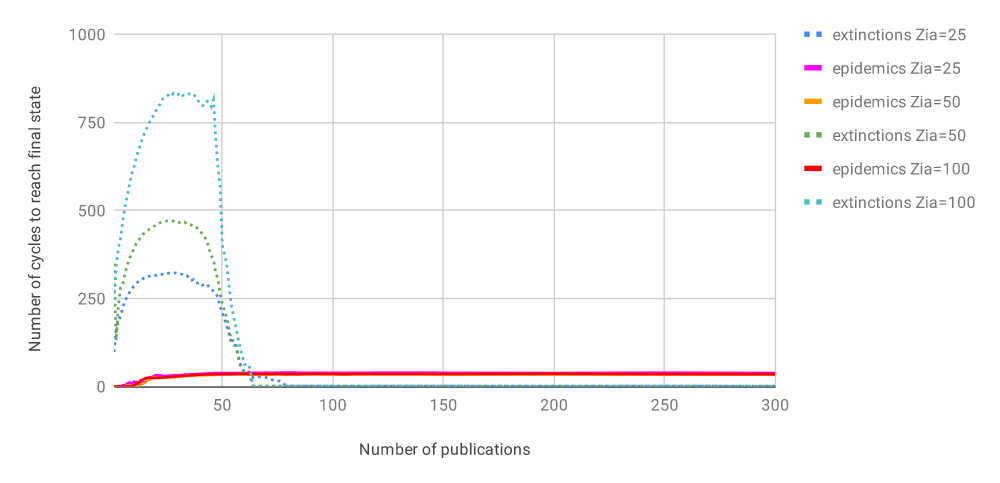
\includegraphics[width=\textwidth]{img/average-number-of-cycles-to-reach-final-state.png}
    \centering
    \caption{Average number of cycles to reach a final outcome}
    \label{fig:average-number-of-cycles}
\end{figure}
An interesting observation relates to the average number of cycles the simulation needs to finish at some final outcome given $Z_{IA}$ (see Figure \ref{fig:average-number-of-cycles}). The average number of cycles needed to reach an extinction grows rapidly until the probability of an extinction is greater than the probability of an epidemic. (Intuitively, the equilibrium point at which the network has the same chance to reach an extinction and an epidemic corresponds to the longest a simulation run can get.) A growing $Z_{IA}$ first increases this number by keeping the nodes in the infected state for a higher number of cycles, then decreases it to zero––indicating that the network can not reach an extinction anymore, or when it does, it reaches it quickly.
The average number of cycles to reach an epidemic is stable at 33 to 38 cycles, perfectly matching the average number of publications needed to reach an epidemic. Intuition tells us that if the network has not reached an epidemic by the time of the last publication (or few cycles after it), there is no chance of reaching an epidemic--the number of external infections was too small.

Another thing that looks strange is that even with many publications, there still exist simulations where the network does not reach an epidemic. To find an explanation of this riddle, we run visual simulation hoping for a clue. This provides us some interesting feedback--some "unfortunate" graph instances and $\xi$ values prevent the whole network from reaching an epidemic even with a large number of external infections (proofs-of-time).
If in a trust graph there exists a \textit{defensive alliance} $A \subseteq N$ of connected nodes where each node $v \in A$ is connected to fewer than $\xi * |N(v)|$ nodes outside $A$, then such an alliance prevents than epidemic. If we assume $\xi = \frac{1}{4}$ and the graph structure visible in \ref{fig:defensive-alliance}a,
\begin{figure}[h!]
  \subfloat[]{
	\begin{minipage}[c][1\width]{
	   0.5\textwidth}
	   \centering
	   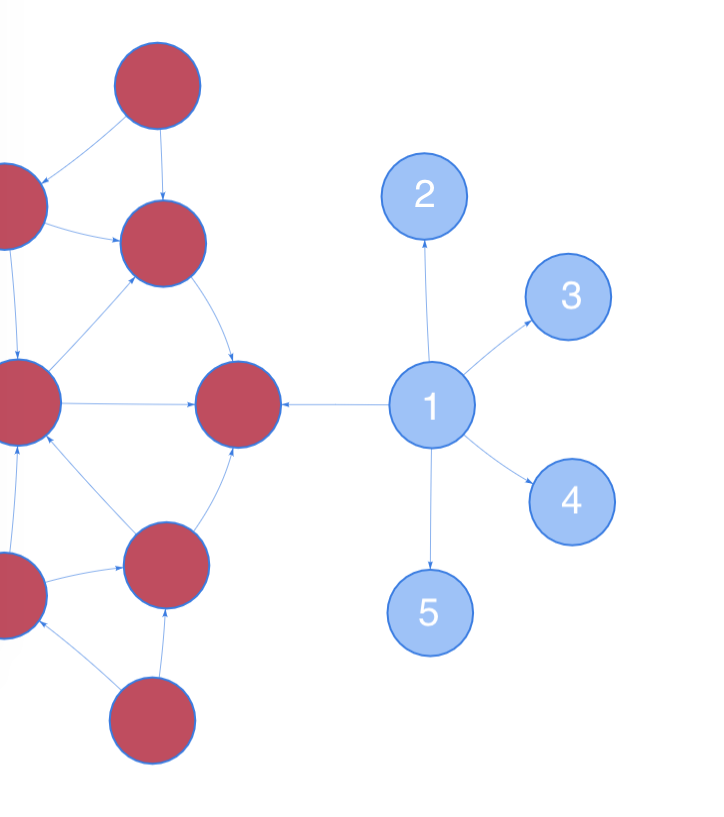
\includegraphics[height=1.0\textwidth]{img/offensive-alliance-numbered.png}
	\end{minipage}}
 \hfill 	
  \subfloat[]{
	\begin{minipage}[c][1\width]{
	   0.5\textwidth}
	   \centering
	   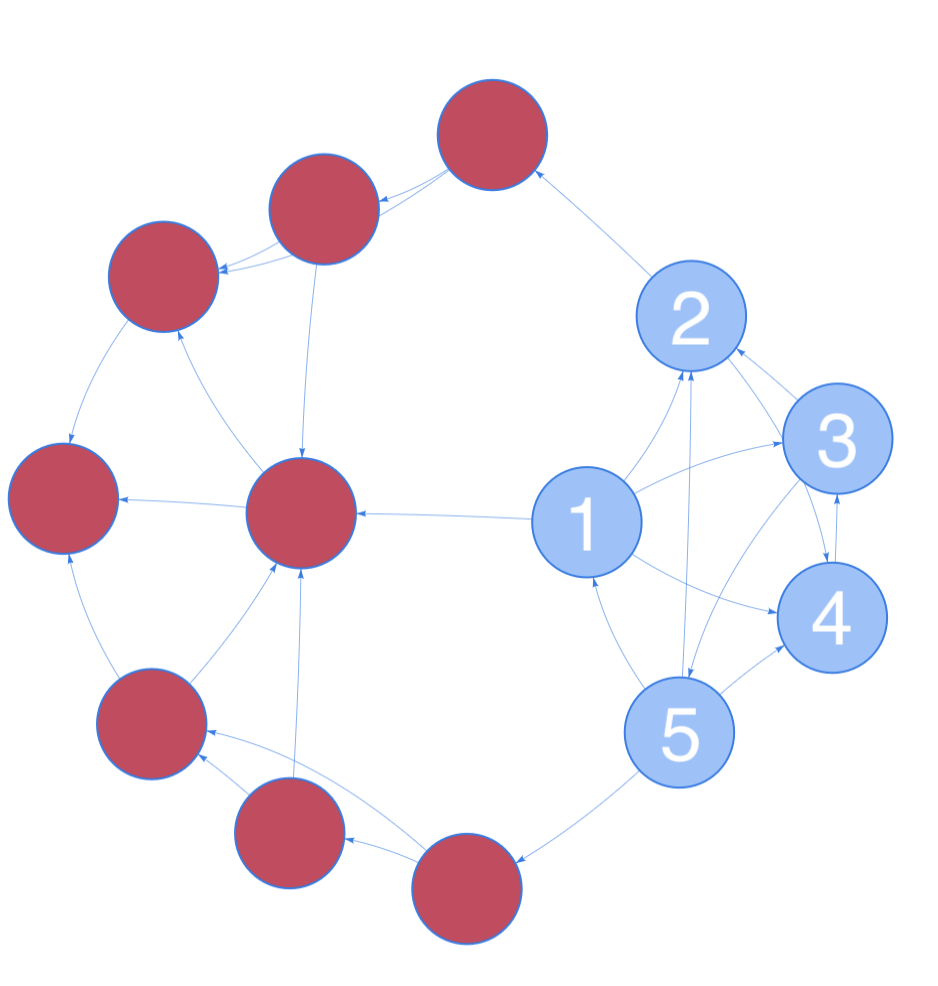
\includegraphics[height=1.0\textwidth]{img/offensive-alliance-clique-numbered.png}
	\end{minipage}}
\caption{Defensive Alliance}
\label{fig:defensive-alliance}
\end{figure}
then the infected nodes (in red) are not able to infect the healthy ones (in blue), especially $v_1$, which is the single node connected to the outside of $A$. It happens because the healthy node $v_1$ has five neighbor nodes, of which four are healthy ($\{v_2,v_3,v_4,v_5\}$), hence the one infected neighbor node is not enough to reach the $\xi = \frac{1}{4}$ threshold at $v_1$.
Let us take a different graph where defensive alliance $A$ is connected to rest of the graph $N \setminus A$ through more than one node as shown in \ref{fig:defensive-alliance}b. Nodes from $A$ cannot be infected since there are not enough connections from outside $A$ to reach the $\xi$ threshold. A general defensive alliance is defined by: 
\begin{equation}
\forall{v \in A}, \frac{|N(v) \cap A|}{|N(v)|} > 1 - \xi.
\end{equation}
As a result, the rest of the network stays in the Acute state until the nodes connected to $A$ change their state to Quarantine (notice that their $\%_n$ are less than 1), which then propagates throughout the rest of the network leading to an extinction. 

To eliminate defensive alliances, we could modify the trust graph generator, but that would violate our assumption that the structure of the trust is taken as a given. Lowering $\xi$ might be another option, but in this way, we would speed up the infection process on the whole network, which is an unwanted effect.

The problem of finding a defensive alliance is NP-complete \cite{ouazine2018alliances}. There is no known solution to finding defensive alliances or even answering in polynomial time whether there exists one in the graph. Therefore the only way of locating defensive alliances in the graph is an exhaustive search. The problem gets even worse if we assume that the network is open, i.e., at any moment nodes can join or leave. 

\chapter{Consensus}
\label{consensus}
If we look at our problem from a different perspective, we notice that we are trying to achieve a consensus among all the nodes about whether the given piece of content is authentic or not. In the graph infection (GI) algorithm, the consensus is dictated by the number of external infections. Too low a number leads to an extinction, whereas a high enough leads to an epidemic. Both an epidemic and an extinction can be considered consensus decisions. In an epidemic, the whole network generates a positive decision about the content authentication, while in an extinction, the network decides the opposite.

% Very important chapter
If we evaluate GI in terms of the consensus problem, it turns out that it struggles with faulty nodes. In GI, each node controls the time after the next external infection is allowed. If a node fails, it can allow immediate propagation or not allow it at all. Additionally, the consensus is not deterministic––there is no guarantee that the network will reach the same final occurrence for each simulation run with the same initial conditions. Although the consensus is achieved using timeout (the $\tau$ parameter specifying the time to immunization), the time to reach a consensus is non-deterministic.

If we consider \textit{Byzantine failures}\cite{lamport2019byzantine} that allow nodes to act arbitrarily (e.g., send corrupted, malicious, or conflicting information to other nodes) then a node can be stuck in either a healthy or infected state, ignoring the state of its neighbors, hence a single faulty node can change the decision of all non-faulty nodes. In consequence, it can prevent the whole network from reaching an extinction or an epidemic. Consider again the graph in Fig. \ref{fig:defensive-alliance}a where all nodes are healthy, node 1 is an adversary and falsifies its state as infected; in this way, it infects nodes ${2,3,4,5}$ which are entirely dependent on node 1; therefore, they will stay infected as long as node 1 decides. 

We evaluate the presented GI protocol using three known consensus requirements: Validity, Agreement, and Termination.
\begin{enumerate}
    \item Validity: any value decided upon must be proposed by one of the nodes.
    \item Agreement: all non-faulty nodes must agree on the same value
    \item Termination: all non-faulty nodes eventually decide.
\end{enumerate}

Validity and Agreement specify what \textit{must not} happen––there cannot be a situation where the consensus is reached on a value that was not proposed by any node (in our case, neither an epidemic nor an extinction). Also, there must be no non-faulty nodes that decide other than the rest of the nodes. In the distributed systems literature \cite{lamport1977proving} those properties are called \textit{safety}. On the other hand, Termination specifies what \textit{must} happen––at some point, all non-faulty nodes must reach a consensus. In the literature, this property is also called \textit{liveness}.

The Validity requirement is stated to avoid trivial consensus algorithms like "always choose 0," which is not the case in the GI protocol.

The Agreement requirement is satisfied owing to the timeout parameter $\tau$ that covers some corner cases involving defensive alliances.

Termination is also satisfied––if the network cannot reach a consensus, then after $\tau$ number of cycles, nodes get immunized leading the whole network to the final occurrence. The longer the simulation takes, the more likely the network is to reach an extinction and less likely to reach an epidemic.

We have seen that in the case of Byzantine failures,  neither fault-tolerance nor safety is satisfied. One single faulty node can prevent non-faulty nodes from deciding on the same value, breaking the safety requirement using one single faulty node.
% Very important chapter
It is probably not impossible to extend the GI algorithm such that it satisfies those properties. If the nodes could gain more awareness of the network state, they could detect faulty nodes and therefore become fault-tolerant. However, it is worth looking at alterntive solutions. 

There are a variety of  consensus algorithms that differ in the allowed types of node failure (Byzantine or not), synchrony (Asynchronous or Synchronous), the number of tolerated failure nodes, authentication (whether messages have to be signed by their authors), and the number of cycles to achieve consensus. 

Instead of looking at the original Stolen Credentials problem as a consensus protocol design problem, we propose a solution that can be deployed on top of an already existing consensus protocol. We search for protocols resilient to Byzantine failures because, for an Internet-level protocol managed by many organizations, we cannot assume that all nodes will act reliably and honestly. Additionally, the protocol must allow open membership--nodes should be able to join and leave the network at any time. 


\chapter{Blockchain}
\label{blockchain}
Consensus protocols that work with Byzantine-failure nodes and allow open membership are used in open Blockchains. By open Blockchain, we understand the Blockchains where nodes can freely join the network and participate in the consensus protocol. Examples of such Blockchains are Bitcoin \cite{nakamoto2008peer}, Ethereum \cite{wood2014ethereum}, and Stellar \cite{mazieres2015stellar}. Bitcoin uses a proof-of-work consensus algorithm where the computational power dictates the contribution to the consensus decision. Ethereum plans to switch to a proof-of-stake consensus where the amount of cryptocurrency dictates the contribution to the consensus decision. Stellar uses federated byzantine agreement where the trust dictates the contribution to the consensus decision. 

Data stored in Blockchain is immutable––once written to Blockchain, no one can change it, data is also secure against the intruders (as long as they do not control the majority of consensus means). Data types differ in different Blockchains, but most of them store the transactions that update the global ledger. Some Blockchains, like Ethereum, also allows storing smart contracts\footnote{Scripts that are executed on virtual machines on all nodes and uses Blockchain as a persistent storage}. In our case, we use Blockchain to store Proof-of-Time claims. 

\section{System proposition}
We propose the system where all or part of the nodes in the network participate in a Blockchain consensus protocol––securely storing common database consisting of Proof-of-Time claims, along with Content Store. Each node can be sure that rest of the network stores the same version of the blockchain database. But the most vital feature for our system is the fact that by using a Blockchain we ensure that a publishers can publish only one Proof-of-Time at a time. Therefore  to authenticate the content, they must proof their access to credentials over long period of time, long enough so the malicious publisher can not afford to do that, while legit publisher can––the statrequirement we base our authentication mechanism on. To achieve it, a publisher wishing to confirm a content authenticity must submit a carefully prepared transaction to a Blockchain network. The transaction––a Proof-of-Time claim––must include:
\begin{itemize}
    \item Hash of the content wishing to authenticate.
    \item Signature on the claim which proves the access to credentials.
    \item Publisher public key, that can be used to verify the signature and identify the publisher.
    \item Hash of the previous block––preventing pre-signing transactions.
\end{itemize}
Graphical illustration of such transaction is presented in Fig. \ref{fig:proof-of-time}.
\begin{figure}[h!]
    \centering
    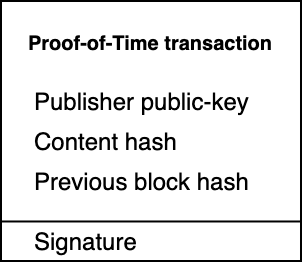
\includegraphics[width=0.4\textwidth]{img/proof-of-time_transaction.png}
    \caption{Structure of Proof-of-Time claim}
    \label{fig:proof-of-time}
\end{figure}

The transaction can then be submitted to a node which include it in a block and broadcast to the rest of the network. Once the block is approved by all network participants (through the consensus protocol described in Sec. \ref{FBA}), the publisher can create next Proof-of-Time transaction pointing to the previous block's hash.    In further chapters we describe the details of the system based on blockchain.

Let's imagine a naive solution based on the Bitcoin blockchain. The solution is naive because Bitcoin's proof-of-work consensus protocol has no practical application in our system. We can not expect resource-constrained network devices to participate in mining process, especially when there are alternatives that achieve security without a mining process. Nevertheless, we decide to explain it on the simplest and most commonly known one. 
Before that, let's recall what we want to achieve. We want the end-user, the content consumer to be sure about the content authentication. We achieve it by requiring the publisher to prove its access to private keys for a long period of time, long enough so the malicious publisher can not afford to do that, while legit publisher can. We call those access proofs––proofs-of-time. In the GI algorithm, the proof-of-time is denoted in a sequential number of external infections. The publisher who can perform long enough proof-of-time lead the network to epidemic, while the short proof-of-time lead to extinction. 

In the blockchain solution, the simplest way to proof access to private-key in the context of some content is to publish transactions from the publisher account to the content account. The content account is the imagined account whose address is the hash of such content. The publisher's account is the same key-pair used to sign the content in the ICN network. The flow is shown in Fig. \ref{fig:distribution-flow}.
\begin{figure}[h!]
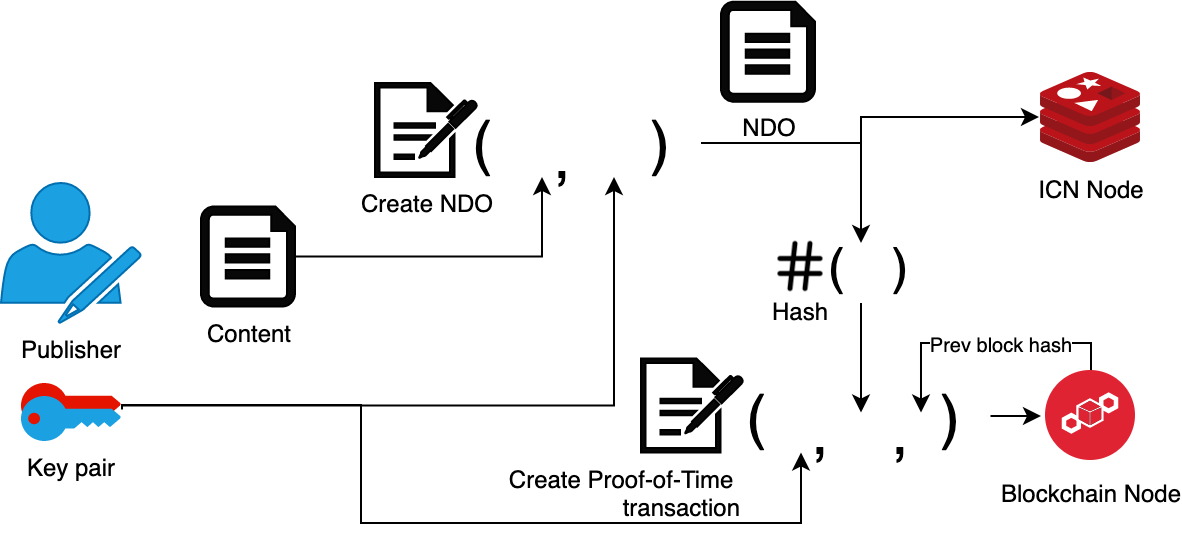
\includegraphics[width=9cm]{img/distribution-flow.png}
\centering
\caption{Flow of publishing content to ICN and proof-of-time to blockchain}
\label{fig:distribution-flow}
\end{figure} 
The strength of the proof-of-time is calculated by counting the total number of transactions to the content hash address. 

Here we will use one of the most fundamental features in Bitcoin blockchain––blocks. Block is a container holding bunch of transactions. Bitcoin is designed to produce a new block every 10min on average, it is achieved by the dynamic complexity of the mining process. If we count each block where the transaction from the publisher account to the content hash exists, we get the strength of proof-of-time that can be interpreted as sufficient to trust the content. This way, the proof-of-time is propagated not as a consensus, but as an overlay structure on top of a trusted immutable database. In Fig. \ref{fig:blockchain-of-claims} we show an example of three blocks consisting of proof-of-time claims. Each block also consists of some meta-data like a hash of its content, a hash of the previous block (pointer to the previous block), and block creation timestamp. We assume that blocks are created with 10min intervals, and each content requires proof-of-time in minimum strength of 20min. Alice first publishes her content to the ICN node getting the hash of the NDO as shown in Figure \ref{fig:distribution-flow}, then the claim is created and published to the Blockchain node. After 10 minutes once again she publishes the claim, and again after another 10 minutes she repeats the process. Three publications in a row certify that Alice had Alice's credentials for at least 20min. Bob was able to publish only two claims, which we consider not enough to trust the content. Carol, on the other hand, skipped the second block which is considered as a break in the proof-of-time chain, therefore we start measuring the proof-of-time from the third block. The algorithm used to process new blocks and check if the content is authenticated is presented in Listing. \ref{listing_process_new_block}.

The mechanism can be extended to the "certification services" (discussed in chapter \ref{mitigating-certification-services}) in such a way that not only the publisher can participate in creating proof-of-time claims, but also some set of trusted units that can certify the content trustworthily–––similar how we trust root CA certificates. 

Attacker who wants to publish bogus content, could pre-sign many proof-of-time transactions and then publish them one by one without access to the credentials. To prevent that, we require from each publisher to provide the hash of the previous block in the transaction. Since the hash of the block is not deterministic for individual publishers, they can not pre-sign transactions. Instead they have to sign the transaction just before sending the transaction to the blockchain.
\begin{figure}[h!]
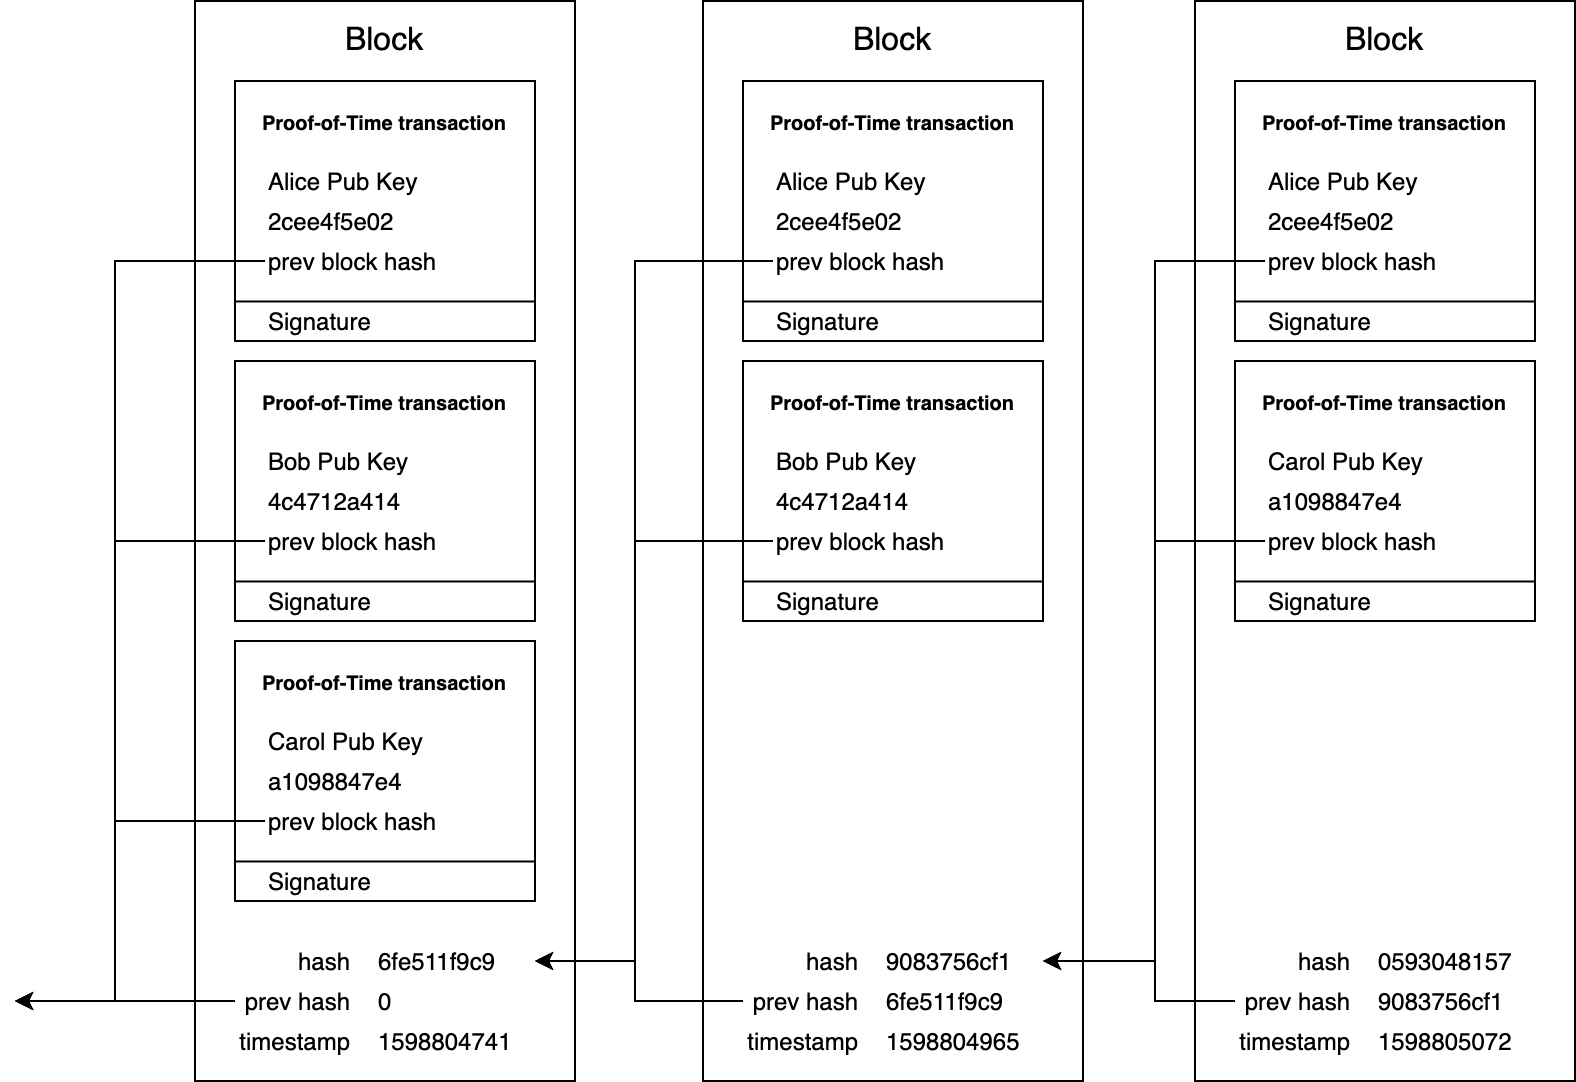
\includegraphics[width=\textwidth]{img/blockchain_of_claims.png}
\centering
\caption{Blockchain of claims}
\label{fig:blockchain-of-claims}
\end{figure} 

\begin{lstlisting}[language=Python, caption=Processing new block, label=listing_process_new_block,float,floatplacement=H]
stored_claims      # { [content-hash] : [publisher_pubkey] : number }
candidating_claims  # { [content-hash] : [publisher_pubkey] : number }
previous_block_hash


def process_new_block(block):
    # handle broken proof-of-time chains
    for content_hash in candidating_claims:
        for publisher_pubkey in candidating_claims[content_hash]:
            if (content_hash, publisher_pubkey) not in block.transactions:
                # proofs-of-time chain has been broken, store the length
                stored_claims[content_hash][publisher_pubkey] = \
                    candidating_claims[content_hash][publisher_pubkey]
                delete candidating_claims[content_hash][publisher_pubkey]

    for transaction in block.transactions:
        content_hash = transaction.hash
        publisher_publickey = transaction.publisher_publickey
        previous_block_hash = transaction.previous_block_hash
        # check the previous_block_hash to prevent pre-signed proofs
        if previous_block_hash != previous_block_hash:
            return
        candidating_claims[content_hash][publisher_publickey] += 1

    previous_block_hash = block.hash


def get_credibility_score(content):
    if stored_claims[content] > candidating_claims[content]:
        return stored_claims[content]
    else:
        return candidating_claims[content]

\end{lstlisting}


As we mentioned earlier, the Bitcoin consensus protocol and any other Nakamoto Consensus––in which the leader capable of updating the blockchain is elected in form of a lottery where the chance of winning is determined by the amount of spent resource––is not suitable for our use case. Fortunately, the topic of distributed systems and especially consensus algorithms are studied for decades so there is a lot to choose from.

\section{Federated Byzantine Agreement}
\label{FBA}
We find Federated Byzantine Agreement (FBA)––and its blockchain Stellar Consensus Protocol (SCP)\cite{mazieres2015stellar}––the most suitable protocol for our needs. In contrast to proof-of-work, where computational power dictates the contribution to consensus, FBA is based on a trust model. That way, it becomes a fast, lightweight, and asymptotic resistant\footnote{the node consisting of large computational power does not gain any advantages in the consensus protocol}. Instead, the contribution value is determined by the node trustworthy––similar to GI protocol. A new node, joining the network, has no contribution to the protocol until someone trusted––start to trust it.
Blockchain like any other asynchronous distributed system faces FLP\cite{fischer1985impossibility} impossibility trilemma––where only two of three properties can be achieved. Those properties are Fault tolerance, Liveness, and Safety. Most systems must be fault tolerance so the choice is left between Liveness and Safety. Safety guarantee state consistency across all nodes in the network. If nodes do not agree on some transaction, they will not split into two different states, but rather wait until the conflict is resolved. Liveness guarantee that the consensus will always terminate and the system will always be available to accept new transactions. When the conflict occurs, the ledger is split into two different versions, until it's resolved, but in the meantime, it can process new transactions. Most of the blockchain protocols choose liveness, tolerating temporary partitioning. They argue that the time of the partitioning is short enough that the users expecting high credibility of the transaction can just wait---until the chance of shifting the state is acceptably small\footnote{In proof-of-work the chance of changing the state of some block gets smaller with the length of the chain of the blocks attached to this block}. The conflict settlement is dictated, again, by computational power. The state which gets the fastest used as a previous block is considered the winner. That way the system can guarantee permanent availability, even with just one working node. 

Stellar Consensus Protocol on the other hand chooses Safety over Liveness. Once the state has been approved, it can not be changed. State gets approved when the quorum of the network agree on the proposed state. This allows much faster confirmation times, in Stellar the ledger closes in about 5 sec. 
Stellar Consensus Protocol is based on Practical Byzantine fault tolerance (PBFT)\cite{castro1999practical}, and extends its functionality by allowing open membership, therefore promoting decentralization. In SCP each node pick its trusted set of nodes called \textit{quorum slice} (in which it is also \textit{ipso facto} a member). The \textit{quorum slice} should be different for each node, but naturally, some nodes are more trustworthy, therefore are chosen more often in the quorum slices. Transitive trust for all node's \textit{quorum-slice} members, forms \texitt{quorum}. For any two quorums, there must exist \textit{quorum-intersection} to prevent network partitioning.

In non-federated byzantine agreement systems, the decision on some state proposal is determined by the majority of the nodes. Once the proposal gets accepted by a quorum (a majority of the nodes), the rest of the network can be sure that other proposals will fail, since they can't reach the quorum, since the nodes can't change their mind. That way the whole network converges to the final outcome.
In decentralized systems, where nodes can join and leave at will, it is hard to know the total number of nodes in the network \texit{a priori}. Therefore it's hard to calculate the majority of the network. Additionally, open systems can not rely on quantitive majority since this would open them to Sybil attacks\footnote{In this attack single entity can join many nodes to the network that looks as independent units, therefore forcing decisions based just on the majority number of nodes}. To solve this issue, FBA introduces the federated voting process that starts locally and expands until it reaches the whole network. To make it work, the local quorums must overlap with at least one node that will convey the voting decisions across different quorums. This property guarantee that if one quorum agrees on some value P, the other quorum can not agree on not-P, because it includes some nodes from the first quorum that already voted on P.

Federated voting starts when some node sends a broadcast to the network announcing a vote on a particular value V. Node sending such value promise that it will never vote against V. Each node sees how other nodes are voting by their broadcast messages. If the node notice that some quorum of nodes voted on value V, it can be sure that such value will be eventually accepted by the whole network (by the definition of quorum), therefore it can switch to \textit{accepting V} state and announce that fact to the whole network, the same way as announced vote decision. Accepting is stronger than voting because voting for V means that the \textit{node} will never vote for non-V while accepting V means that the \textit{each node in the network} will never accept non-V. When a node notices some quorum of nodes accepting V, it \textit{confirms V}, and by the definition of the quorum, all nodes in the network will eventually confirm value V, ending the process of federated voting.

The problem arises, when such nodes which are in quorum intersection are Byzantine-failed, lying about the decisions made on each quorum. In SCP whitepaper, there is an assumption that the network is configured in such a way that even if the malicious nodes are removed from the network, it still holds quorum-intersection. If it does not hold, the network halts until the quorum-slices are reconfigured.
We can only \textit{expect} the network to form connections where there always exist quorum-intersection because the internet––that we are designing the protocol for––itself satisfy such property.

Another problem in an attempt to apply FBA to our use case might be the problem of the DoS attack. A malicious client might publish a huge number of proof-of-time claims successfully leading to network congestion. Stellar prevents that by introducing the transaction fees, therefore attacker is discouraged by financial means. Here in our approach, we don't want to introduce any financial aspects, so other mechanisms must be used to prevent it. DoS is a vital problem in ICN networking in general\cite{gasti2013and}, so the solutions that will be worked out will also solve our problems. 

There are several different blockchain consensus protocols, but not all of them are suitable for internet level protocol and to be run on network devices.
If we consider network devices similar to IoT devices we can leverage the research done on this kind of protocols \cite{salimitari2018survey}. The paper suggests that Stellar consensus is not ideal for IoT devices since it is too slow.
Since the proof-of-time claims are not the matter for milliseconds, but rather minuter or hours, we believe that the protocol is fast enough for our needs.
Also, there already exists a proposal of a modified FBA algorithm\cite{FCPpdf50:online} that uses a virtual voting algorithm that can achieve consensus in almost no communication overhead. We find this topic interested, and plan to research it in future work.

In that paper, the authors suggest that there is a subset of protocols especially suitable for IoT networks. Those protocols are Proof of Elapsed Time (PoET), Practical Byzantine Fault Tolerance (PBFT), and Tangle.

\section{Credibility Score}
In the GI algorithm, there are two states of content authenticity: authenticated or not-authenticated. We believe that this is limiting. Content like e.g. weather forecasting should not be authenticated for the same amount of time as an online banking website. Therefore we propose a more flexible model, where authentication can be acquired progressively via Credibility Score. Credibility Score mentioned in Section \ref{proof-of-time} increase authentication granularity. Pictures, music, movies do not require as much trust as websites where we enter our credentials and credit card details. Different thresholds should be used for different content types. For example, if 3 trust thresholds are used: low, medium, high; then we can require 10min, 2h, 12h of proofs of time accordingly. Each time the content is published to the network the author can be notified about that fact, and if the publisher used stolen credentials, the actual author has a time frame to revoke the credentials and halt the malicious authentication process.

\section{Blockchain layer}
In our proposition nodes in the network plays two roles, an ICN node where it participates in routing and content caching, and as blockchain node where he participates in consensus and blockchain storage (see Fig. \ref{fig:combined_layers}). Not every node has to play two roles, the ones which are not connected to end-uses might not participate in the blockchain network, since they don't get asked for content trustworthy. 
The blockchain layer could also be managed by completely different entities, separating the transport layer from the trust layer (see Fig. \ref{fig:separated_layers}). That way the ICN nodes could be abstracted from the trust network overhead introduced by the trust system––keeping them simpler. Also, the trust system would be more portable, it could be used in many different ICN solutions, and even in legacy systems since the trust does not depend on ICN, but on the hash of the content and publisher credentials. That way the blockchain trust network could be hosted by more powerful devices and possible different organizations––achieving separation of concerns which is always a good thing in the long term.

\begin{figure}[h!]
\centering
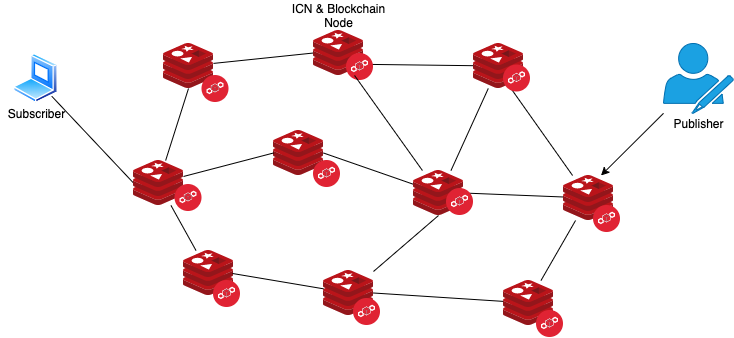
\includegraphics[width=1\textwidth]{img/combined-layers.png}
\caption{Combined layers}
\label{fig:combined_layers}
\end{figure}

\begin{figure}[h!]
\centering
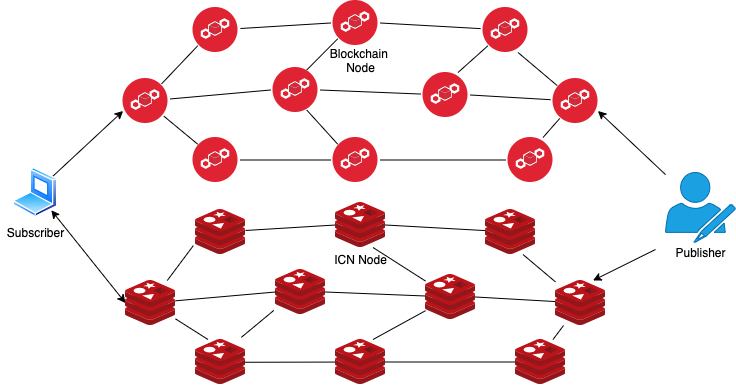
\includegraphics[width=1\textwidth]{img/separated-layers.png}
\caption{Separated layers}
\label{fig:separated_layers}
\end{figure}

%\section{Transaction throughput}
%Transaction throughput––measured in transactions per second––is one of the biggest problems in the blockchain ecosystem. Bitcoin public network can process up to 7 transactions per second (TPS), Ethereum can process 15TPS and Stellar can process 200TPS. The limitation comes from the practical aspects of the system. If we want the system to be decentralized, we can not require all nodes in the network to be super-computers, both in processing power and storage capacity. In our case, we design the system for network devices that have limited resources.

\section{Storage}
Typically blockchain nodes stores whole blocks that consists of bunch of transactions. Our system does not need to store whole transaction (Proof-of-Time claims) history. There is no need to do so. After the sequence of Proof-of-Times is broken, nodes can prune their databases from that transactions, storing only the length of the sequence.

\chapter{Comparison}
\label{comparison}
In comparing the two presented approaches, GI and Blockchain, we have focused on five main characteristics referred to as outcome, resilience, communication complexity, processing scalability (measured by the pieces of content the entire system can handle at a time), and fault-tolerance. One also has to consider the implementation requirements in terms of overlay IT infrastructure. We present the comparison in Table \ref{table:comparison}.
\begin{itemize}

    \item Outcome -- GI is indeterministic when it comes to a consensus decision. Even a high number of proof-of-times can sometimes result in an extinction, which is an unwanted property. Blockchain, on the other hand, is deterministic; a publisher with a high number of proof-of-time claims can be sure that his/her content will be authenticated. This is guaranteed by the safety property of FBA.
    
    \item Resilience -- GI is sensitive to both chance, the network size and structure, and the $\xi$, and $Z_{IA}$ parameters. While Blockchain––particularly using FBA––has just one assumption regarding the quorums-intersection property. We state that Blockchain is more resilient.
    
    \item Communication complexity -- In GI, each node has to communicate with just a constant number of its neighbors, so the complexity is linear in the number of nodes––$O(|N|)$. In Blockchain, each node has to communicate with all other nodes in the network, so the communication complexity is quadratic in the number of nodes––$O(|N|^2)$. In this regard, GI prevails.
    
    \item Processing capability -- to achieve safety, Blockchain has each network node process each piece of content sequentially, so the system is as fast as a single node in the network. Hence, adding nodes does not increase the total processing capability, which therefore is constant in the number of network nodes. In GI, communicates only with its neighbors. Therefore, nodes that are not connected can process different pieces of content independently--more network nodes increase the total processing capability, which is therefore linear in the number of network nodes.
    
    \item Fault-tolerance -- GI in its raw form does not handle fail-stop, let alone Byzantine faults. Blockchain tolerates up to $\frac{|N|-1}{3}$ Byzantine nodes, similarly as Stellar FBA. Blockchain therefore outperforms GI in this regard.
    
\end{itemize}

\begin{table}[h!]
\centering
\begin{tabular}{ || m{3cm3cm} | m{5cm}6cm}| m{5cm6cm} || }
\hline
\hline
Property & GI & Blockchain \\
\hline\hline
Outcome & Indeterministic & Deterministic \\
\hline
Resilience & Depends on chance, $|N|$, $\xi$ and $Z_{IA}$ parameters, network structure (defensive alliance-sensitive) & Depends on network structure (quorums-intersection required) \\
\hline
Communication complexity & $O(|N|)$ & $O(|N|^2)$ \\
\hline
Processing Scaplability & $O(|N|)$ & $O(1)$ \\
\hline
Fault-tolerance & None & Byzantine-fault tolerance up to $\frac{|N|-1}{3}$ faulty nodes \\
\hline
Required overlay infrastructure & NDN, PKI & NDN, PKI, and blockchain network \\
\hline
\end{tabular}
\caption{Comparison of GI and Blockchain}
\label{table:comparison}
\end{table}

\chapter{Summary}
We have elaborated on the Stolen-Credentials Cpntent Poisoning Attack problem proposed in \cite{konorski2019mitigating}. Assuming time- constrained operation of a potential malicious publisher, we have quantified the effectiveness of the existing graph infection-based GI protocol and proposed an alternative, blockchain-based approach. The presence of the time constraint allows to extend the authentication abstraction from \textit{access to credentials} to both \textit{access to credentials} and \textit{access to time}, coining the term \textit{Proof of Time}. We have developed simulators and analyzed the proof-of-time implementation based on GI. Among others, we have observed that GI struggles with the Defensive Alliance problem described in Section \ref{observations}, and remarked on GI's sensitivity to the parameter configuration ($\xi$ and $Z_{ia}$), which may be troublesome in Internet-level graph structures can change in time. Then we have generalize the considerations to a distributed consensus problem and proposed a solution based on Blockchain technology. Besides solving the consensus problem, it also offers valuable properties such as security, integrity, immutability, and Byzantine-fault tolerance. We have proposed a scheme in which the content authentication mechanism is embedded not in the consensus mechanism, but as an overlay structure (blockchain) on top of the consensus algorithm. In consequence, we gain a deterministic and reliable authentication mechanism called Credibility Score. We have found Stellar and its Federated Byzantine Agreement consensus protocol to be a blockchain implementation most suitable for our needs. One disadvantage of it is the quorum-intersection requirement described in Section \ref{FBA}. Additionally, the Blockchain solution is more demanding in terms of overlay infrastructure and does not scale well with the network size.
We believe that authentication schemes based on proof-of-time may become a valuable option for the future development of ICN environments.


%\defbibheading{bibliography}[\bibname]{\chapter*{#1}}

% WYKAZ LITERATURY
\clearpage\phantomsection
\addcontentsline{toc}{chapter}{\textbf{Bibliography}}
\printbibliography[title={Bibliography}]

% WYKAZ RYSUNKÓW
\clearpage\phantomsection
\addcontentsline{toc}{chapter}{\textbf{List of Figures}} %{\listfigurename}
\listoffigures

% WYKAZ TABEL
\clearpage\phantomsection
\addcontentsline{toc}{chapter}{\textbf{List of Tables}} %{\listtablename}
\listoftables

% DODATKI
% formatowanie naglowkow dodatkow
\renewcommand\theHchapter{\Alph{chapter}}
\renewcommand\thechapter{\Alph{chapter}}                % chapter number in alph letters
\renewcommand\thesection{\Alph{chapter}.\arabic{section}} % make sections "A.I"
\setcounter{chapter}{0}                                  % start numbering chapters from 1 on again
\titleformat{\chapter}{\large\bfseries}{\MakeUppercase{\appendixname~\thechapter.~\currentname}}{0.5em}{}

\titlecontents{chapter}[0cm]{}{\normalsize\bfseries{Appendix\space}\contentslabel{-1pt}\hspace*{0.6cm}}{}{\titlerule*[3pt]{.}\hspace*{5pt}\contentspage}

\input{Appendices/AppendicesMain}


% Wykaz ważniejszych oznaczeń i skrótów
\chapter*{Streszczenie 2}
Praca została rozpoczęta od wprowadzenia do sieci Informacjo-centrycznych. Zasada działania została opisana na przykładzie projektu Named Data Networking (NDN). Następnie przedstawione zostały problemy z jakimi zmagają się sieci ICN. Jednym z nich jest atak zatruwania treści (ang. Content Posioning Attack (CPA)), a zwłaszcza jego silniejsza forma––atak zatruwania treści przez fałszywe dane (ang. Fake Data CPA). W celu inspiracji wykonany został przegląd innych technologii które również zmagają się z problemem zatruwania treści, a dokładniej Wikipedia, LOCKSS, oraz media społecznościowe. Te ostatnie pozwalają dostrzec podobieństwa między Fake New-sami, a zatruwaniem treści. Zaproponowane zostało rozwiązane problemu Fake News-ów bazujące na czasie dostępu Fake News-a w miejscu w którym jego żywotność jest ograniczona. Następnie rozwiązanie to zostało uogólnione do metody uwierzytelniania treści, nie tylko w mediach społecznościowych, ale również w sieciach ICN. Uogólnione rozwiązanie nazwane Dowód-Czasu (ang. Proof-of-Time) polega na rozszerzeniu mechanizmu uwierzytelniania treści o składnik dostępu czasowego do uwierzytelnień pozwalających na publikacje danych.
Następnie bazując na pracy \cite{konorski2019mitigating} zbadany został algorytm infekcji na grafach w celu implementacji wcześniej założonego mechanizmu. Przebadane zostały różne modele używane w epidemiologii które pozwalają na symulację oraz analizę procesów epidemiologicznych.
Kolejno przebadane zostały struktury grafów oraz algorytmy genratorów pozwalające na budowę sieci o różnych właściwościach m.in. sieci bezskalowe. 

Kolejny rozdział poświęcony został przeglądowi ataków na dane uwierzytelniające. Informacja ta, pozwala na oszacowanie wymaganego dostępu czasowego do uwierzytelnień w celu efektywnego działania mechanizmu Dowodu-Czasu.

Następny rozdział szczegółowo opisuje zasade działania algorytmu infekcji na grafach, w szczególności opisuje maszyne stanów która steruje zachowaniem każdego węzła w sieci. Opisuje również mechanizm rozprzestrzeniania się infekcji.

Stworzone na cele tej pracy simulatory pozwalają na dogłębną analizę algorytmu, oraz na obserwacje anomalii. Jedną z takich anomali jest zjawisko zwane Sojuszem Defensywnym, który skutecznie może zablokować rozprzestrzenianie się epidemii––co w przypadku tego algorytmu jest niechcianym efektem. 

Następny problem infekcji na grafach zostaje uogólniony do problemu konsensusu. Zauważone zostaje ze końcowy stan sieci -- epidemia lub wygaśnięcie, może być interpretowany jako decyzja wypracowana na drodze konsensusu wszystkich węzłów sieci. Z tegorozdział generalizuje problem infekcji na grafach do problemu konsensusu. Wezły powodu problem ten może być rozwiązany używając również innych algorytmów konsensusu.

Zaproponowany został 

We started this thesis from formulating the problem of Fake Data CPA. It turns out that Fake Data CPA is a hard problem, but assuming certain conditions (time constraints), we proved that it is solvable. Time constrain allows us to extend the authentication from \textit{access to credentials} to both \textit{access to credentials} and \textit{access to time}. We call the access to credentials over some time the \textit{Proof of Time}. We build simulators and analyzed the proof-of-time implementation based on graph infections proposed in \cite{konorski2019mitigating} and found some interesting observations. The graph infections algorithm struggle with the Defensive Alliance problem described in Section \ref{observations}. Also, we doubt if its configuration (parameters $\xi$ and $Z_{ia}$) sensitivity is suitable for internet level networks where the structure can change. We also point out the lack of both fail-stop and Byzantine-fault tolerance property. Then we generalize the problem to a distributed system consensus problem and propose a solution based on blockchain technology. Besides the fact that blockchain as a distributed system solves the consensus problem, it also offers valuable properties such as immutability and security. We propose a scheme in which the content authentication mechanism is embedded not in the consensus mechanism, but as an overlay structure on top of the consensus algorithm. In consequence, we gain the deterministic and progressive authentication. We found Stellar and its Federated Byzantine Agreement consensus protocol to be the most suitable blockchain implementation to our needs, it does not require mining or any other market forces to achieve security. One disadvantage is the disjoint-quorums problem described in Section \ref{FBA}. Additionally, the blockchain solution is more complex, introduces more communication overhead, and does not scale horizontally.

We believe that authentication schemas based on proof-of-time may become a valuable option for the future development of ICN networks. 



\end{document}
%%%%%% ------------------------------------- %%%%%%
%%%%%% WLASCIWY DOKUMENT - STOP %%%%%%